\documentclass[12pt]{jsbook}
\usepackage{pethesis}
\usepackage{amsmath,amssymb,bm}
\usepackage{subfigure}
\usepackage{cite}
\usepackage{minitoc}
\usepackage{hhline}
\usepackage{slashbox}
\usepackage{booktabs}
\usepackage[dvipdfmx, usenames]{color}
\usepackage{comment}
\usepackage{ulem}
\usepackage{url}
\renewcommand\UrlFont{\rmfamily}
\usepackage{algorithm}
\usepackage{algorithmic}
\usepackage{color}
\usepackage{latexsym}
\usepackage{ascmac}
\usepackage{subfig}
\usepackage{xbmkanji}
\usepackage[labelsep=quad]{caption}
\usepackage{color}
%\usepackage{otf}

\renewcommand{\refname}{}

\newcommand\whline{%
     \noalign{\xdef\origarrayrulewidth{\the\arrayrulewidth}%
     \global\arrayrulewidth 3\arrayrulewidth}%
     \hline%
     \noalign{\global\arrayrulewidth\origarrayrulewidth}%
}

%%%%%%%%%%%%%%%%%%%%%%%%%%%%%%%%%%%%%%%%
\newif\iffigure
%\figurefalse
\figuretrue
%%%%%%%%%%%%%%%%%%%%%%%%%%%%%%%%%%%%%%%%

% SYMBOL DEFINITIONS
\newcommand{\uvec}[1]{\boldsymbol{\hat{\textbf{#1}}}}
\newcommand{\matr}[1]{\mathtt{#1}}
\newcommand{\img}[1]{\mathbb{#1}}
\newcommand{\argmin}{\mathop{\rm arg~min}\limits}
%\newcommand{\bm}[1]{{\mbox{\boldmath $#1$}}}

%\setlength{\subfigtopskip}{-10pt}
%\setlength{\subfigcapskip}{-10pt}
%\setlength{\subfigbottomskip}{-10pt}
%\setlength{\abovecaptionskip}{-10pt}
%\setlength{\belowcaptionskip}{-10pt}

%
% 論文の表紙の項目
%
\thesistype{2019年度 修士論文}
\title{\vspace{-7mm}直線特徴に基づく\\全天球カメラの高速な位置姿勢推定}
\etitle{Fast Localization of Spherical Camera \\Using Line Information}
\affiliation{東京大学大学院 工学系研究科 精密工学専攻}
\supervisor{山下 淳 准教授}
\studentid{37-186282}
\author{野田 純平}

\begin{document}
\dominitoc
%表紙
\maketitle
%概要
%\thispagestyle{empty}
%\thispagestyle{empty}
%\chapter*{概要}
\markboth{概要}{}
\label{abst}
\def\thepage{}
\thispagestyle{empty}

人間が直接作業することの困難な環境では,ロボットを用いて作業を行うことが期待されている.このとき,作業位置を特定するなどの目的でロボットの運動を推定することが求められる.例えば,ロボットを用いた橋梁の点検では,点検箇所を把握することが必要であり,画像情報を用いたロボットの運動推定に関する研究が行われている[1].橋梁点検などのように,作業対象物に近接した状態においてより多くの情報を取得するためには,視野の限られた通常のカメラよりも視野の広いカメラが適している.本研究では,周囲360◦ の情報を一度に取得できる極めて広い視野を有する全天球カメラに注目する.\\
全天球カメラを用いた運動推定の研究として,Structurefrom Motion(SfM)による手法が提案されている[2].SfM は,カメラ1 台の移動によって異なる視点からの画像を取得し,3次元復元と運動推定を行う手法である[3].橋梁の点検においては,点検箇所を把握するために絶対的な移動距離を推定することが求められる.しかしSfM には,スケールの不定性や,カメラの移動量が小さい場合に運動推定精度が低下するという問題がある.\\
その他の運動推定の研究として,複数台のカメラを用いたステレオカメラによる3次元計測の結果を利用する運動推定の手法が提案されている[4].基線長が固定されているステレオカメラによる運動推定の性質として,上述のスケールの不定性や,カメラの移動量が小さい場合の運動推定精度の低下という問題は生じない.しかし,[4] は通常のカメラを用いており,全天球カメラの広い視野を活用したステレオによる運動推定の手法は構築されていない.\\
視野の広いカメラを複数台用いた3次元計測の研究としては,複数台の魚眼カメラを用いた手法が提案されている[5].しかし,[5] は対応点を曲線上で探索しており,また180◦ 程度の範囲のみを取得する魚眼ステレオカメラを用いて運動推定を行う場合,移動前後での計測に共通部分が含まれずに運動が推定できない場合が生じうるという問題がある.全天球カメラを用いた場合には,対応点の探索を直線上で行うことができ,またカメラがどのような移動をしても必ず共通部分が得られて運動を推定することができる.\\
本研究では,全天球ステレオカメラを用いた3次元計測結果を利用する運動推定の手法の構築を目的とする.ステレオカメラとの幾何的な関係から計測における誤差が大きいような点を,信頼度が低いとして除去することで運動推定の精度を向上させる手法を提案する.

本論文では全天球ステレオカメラの運動推定手法を構築した.
まず提案手法において基本となる2視点の画像を用いた手法について述べた.
この手法では,カメラの前に配置する透明平板の姿勢は任意とした.
しかし,この手法において透明平板をカメラの光軸と垂直に配置した場合,
特殊なケースとして扱えることが明らかとなり,その特殊性を利用して改良し,
透明平板がカメラ光軸に垂直な場合の手法として確立した.
これは平板の姿勢を任意とした場合の手法に比べ,必要な対応点数が1つ減るという特徴がある.
上述の手法はいずれも2視点間の関係のみを用いた手法であったため,
最後に前述の手法を多視点に拡張し,かつ得られた3次元情報を最適化するためのバンドル調整を用いた手法について述べた.
提案手法では屈折が発生しているため,この効果を考慮した新しい誤差関数を定義した.
なお,このバンドル調整には初期値が必要であり,前述の2視点でスケール復元が可能な手法により得られた値を初期値とした.
これにより,2視点だけでなく多視点の画像を用いて最適化が可能となり,かつ最適化処理を入れることでよりロバスト性の高い手法となった.

次に提案手法の有効性を示すため,実験を行った.
その結果,提案手法は対応点座標値の誤差に影響を受けやすいことが分かった.しかし,バンドル調整を用いた手法において,
視点の数を増やすことでこの誤差に対するロバスト性が向上することが示された.一方で,透明平板を厚くすること,解像度の高いカメラを用いることが
精度の高い計測を行うために重要であることも明らかとなった.
実画像を用いた実測実験では,実際にカメラの前に透明平板を配置した状態で撮影した画像に対して
提案手法を適用した.その結果高い精度で計測対象のスケールを復元することができ,
提案手法が有効であることが示された.

\thispagestyle{empty}

\newpage
%%%%%%%%%%%%%%%%%%%%%%%%%%%%%%%%%%%%%%%%%%%%%%%%%%%%%%%%%%%%%%%%%%%%%%%%%%%%%%%

%%%%%%%%%%%%%%%%%%%%%%%%%%%%%%%%%%%%%%%%%%%%%%%%%%%%%%%%%%%%%%%%%%%%%%%%%%%%%%%
%%% Local Variables:
%%% mode: katex
%%% TeX-master: "../thesis"
%%% End:


\frontmatter
%目次
\tableofcontents
%図目次
\listoffigures
%表目次
\listoftables

%
%以下本文
{\mainmatter
\setcounter{page}{1}
\chapter{���_}
\label{chap:introduction}
\minitoc

\thispagestyle{empty}

\newpage
%%%%%%%%%%%%%%%%%%%%%%%%%%%%%%%%%%%%%%%%%%%%%%%%%%%%%%%%%%%%%%%%%%%%%%%%%%%%%%%%%%%%%%%%%%%%%%%%%%%%%%%%%%%%%%%%%%%%%%%%%%%%%%%%%%%
\section{�w�i}
\label{sec:background}

�I�[�����Ƃ́C�}\ref{fig:aurora}�Ɏ����悤�Ȓn���̋ɒn�t�߂̏��Ŋϑ�������C�̔������ۂł���D
�I�[�����͐F�▾�邳�C������`��Ȃnj������̎�ނɕx�݁C���̐_��I�Ȕ�������_�C�i�~�b�N������L����ʂɒm���Ă���D
�Â�����I�[�����ɑ΂���֐S�͍����C���{�⒆���ɂ����Ă�7���I������I�[�����Ǝv���錻�ۂɂ‚��Ă̋L�^�����j���ɋL����Ă���\cite{�F���J1988}\cite{hayakawa2016}�D
�ߔN�ɂ����Ă��I�[�����̉f���R���e���c�ɑ΂�����v�͑傫���C�C���^�[�l�b�g��ʂ������A���^�C���ł̃I�[�����ӏ�\cite{�V��}��C�F���X�e�[�V��������B�e���ꂽ�I�[����4K����̌��J\cite{NASA2016}�Ȃǂ̐V�������g�݂��ϋɓI�ɍs���Ă���D
�ȏ�̂悤�ɃI�[�����͎�����킸�l�X�̊֐S���W�߂Ă��鎩�R���ۂł��邪�C���̔������J�j�Y���Ɋւ��Ă͖����𖾂���Ă��Ȃ������������C���݂������Ɍ�������Ă���D\\

\iffigure
\begin{figure}[b]
\begin{center}
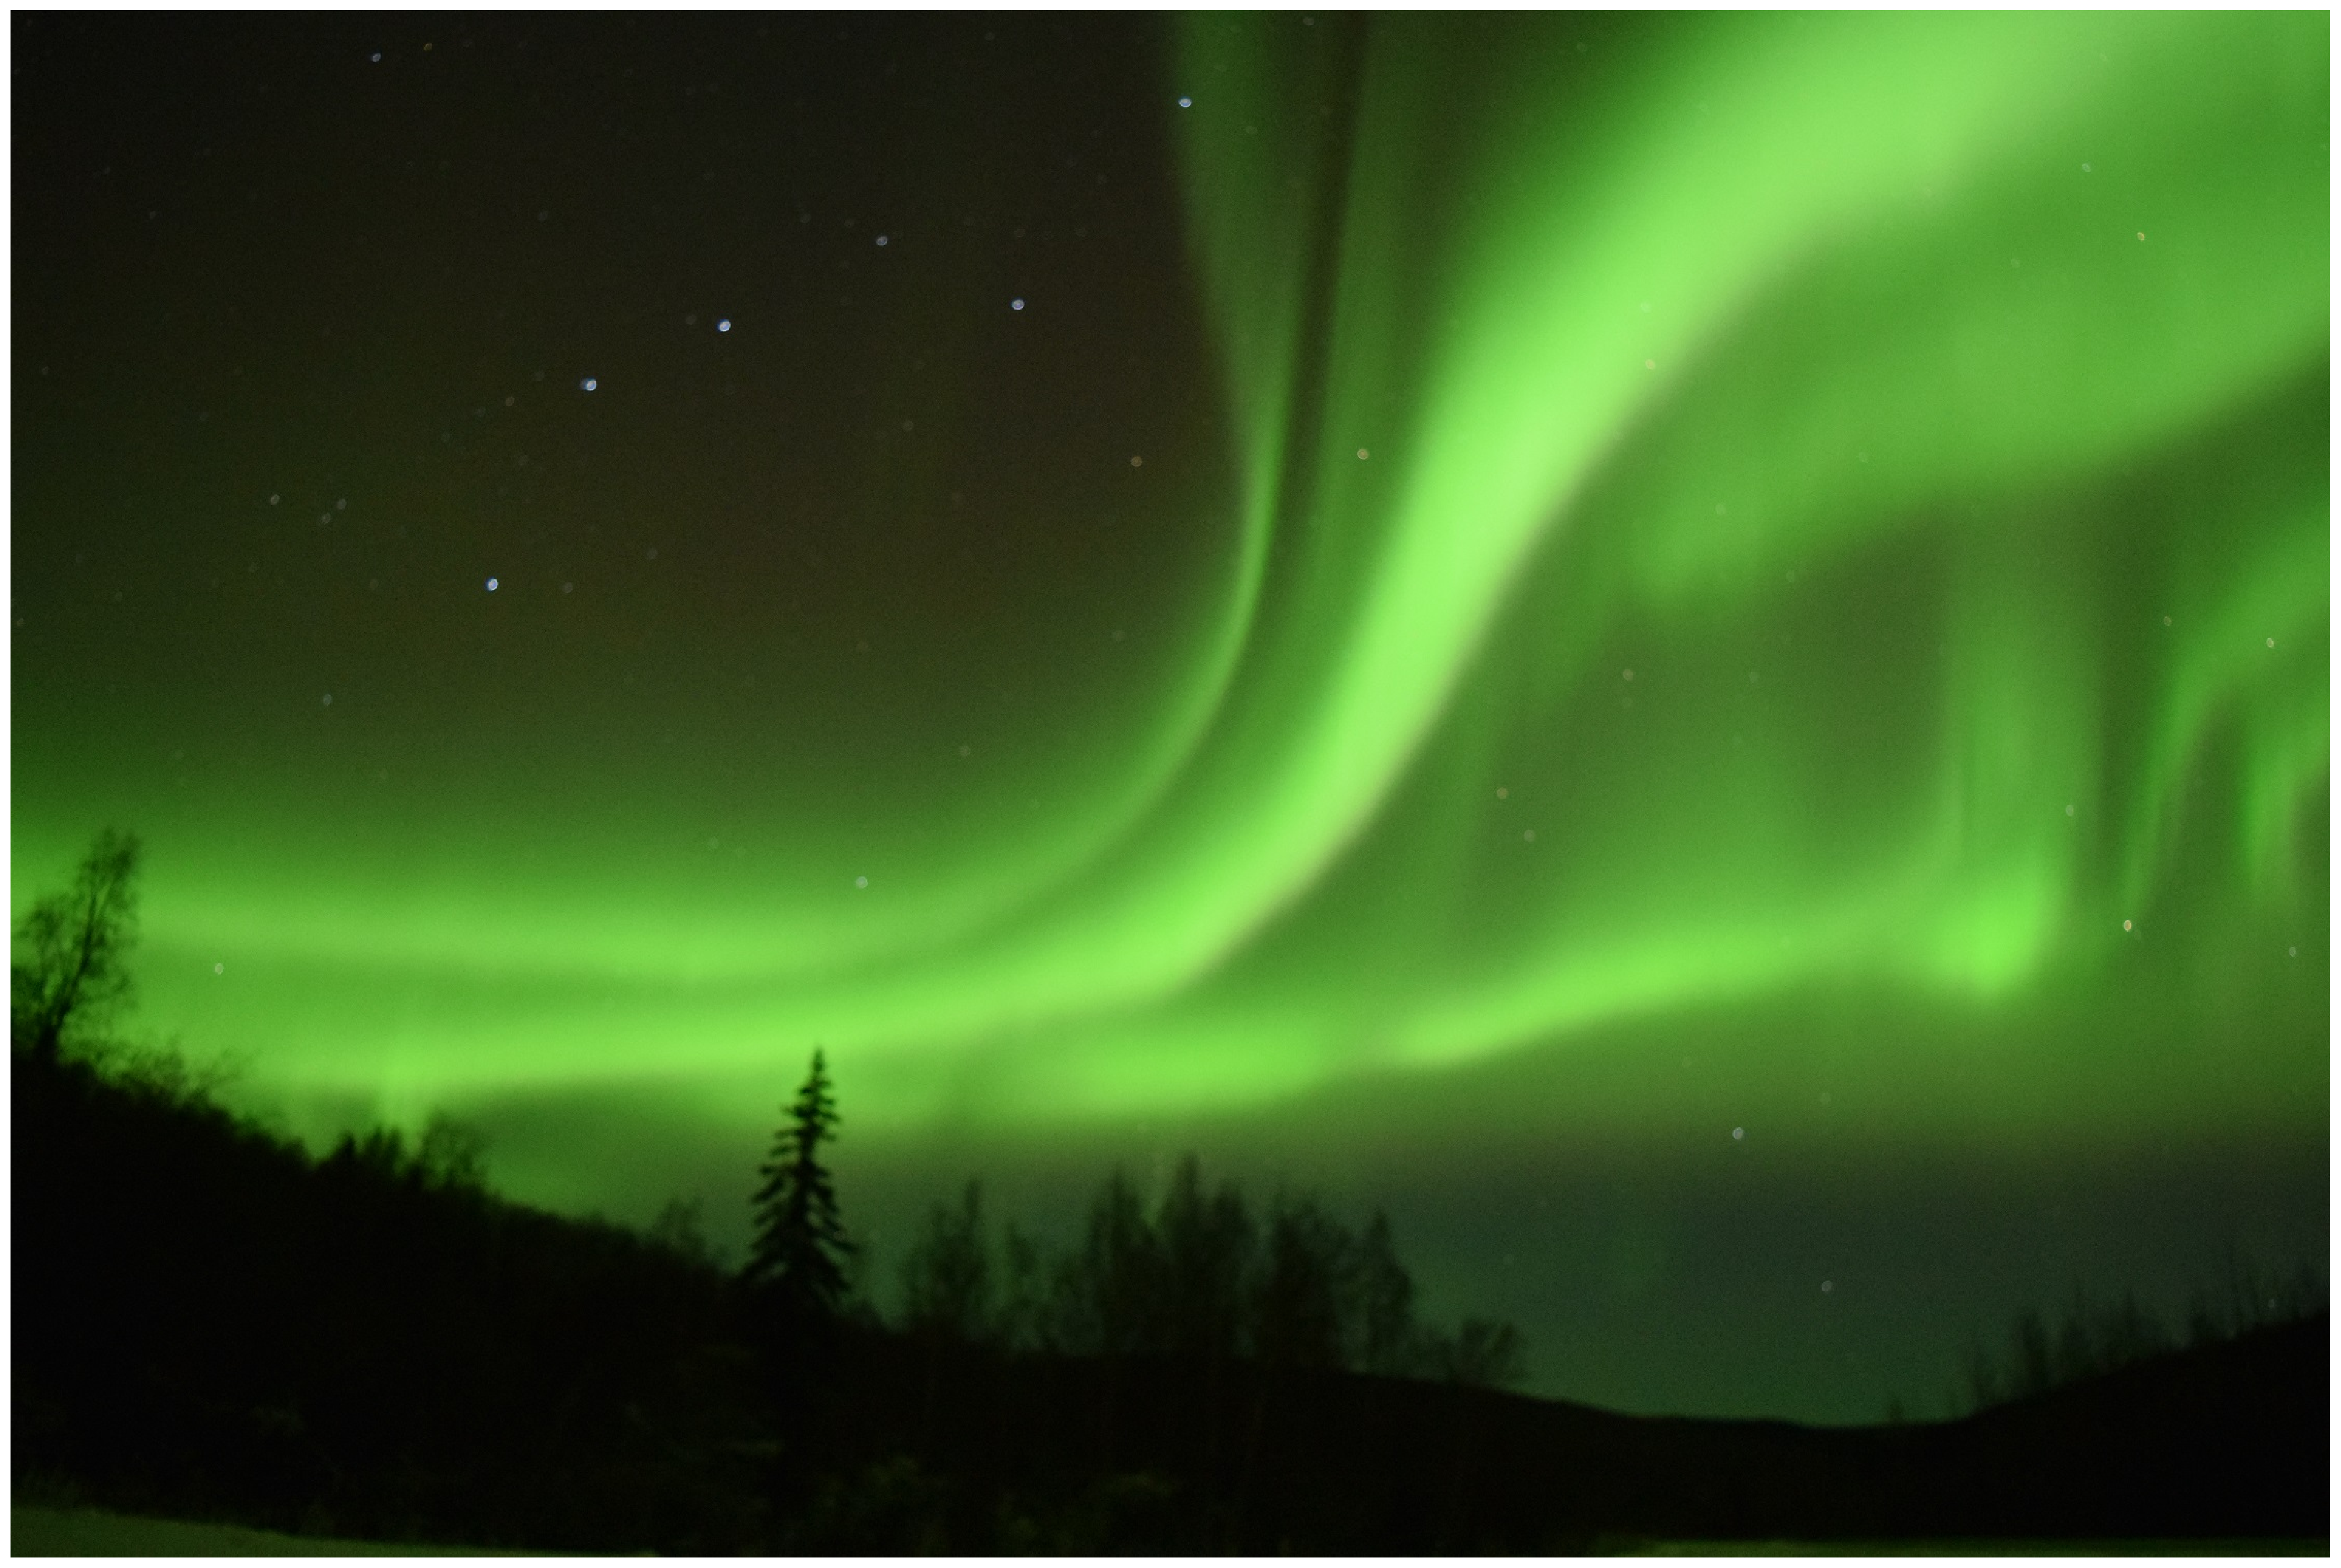
\includegraphics[width=10cm]{./chap1/eps/AuroraExample.eps}
\caption{�I�[�����̗�i2014�N11���C�t�F�A�o���N�X�ɂĎB�e�j}
\label{fig:aurora}
\end{center}
\end{figure}
\fi

\iffigure
\begin{figure}[tb]
  \centering
  \subfigure[�v���Y�}���q�̒~��]{
    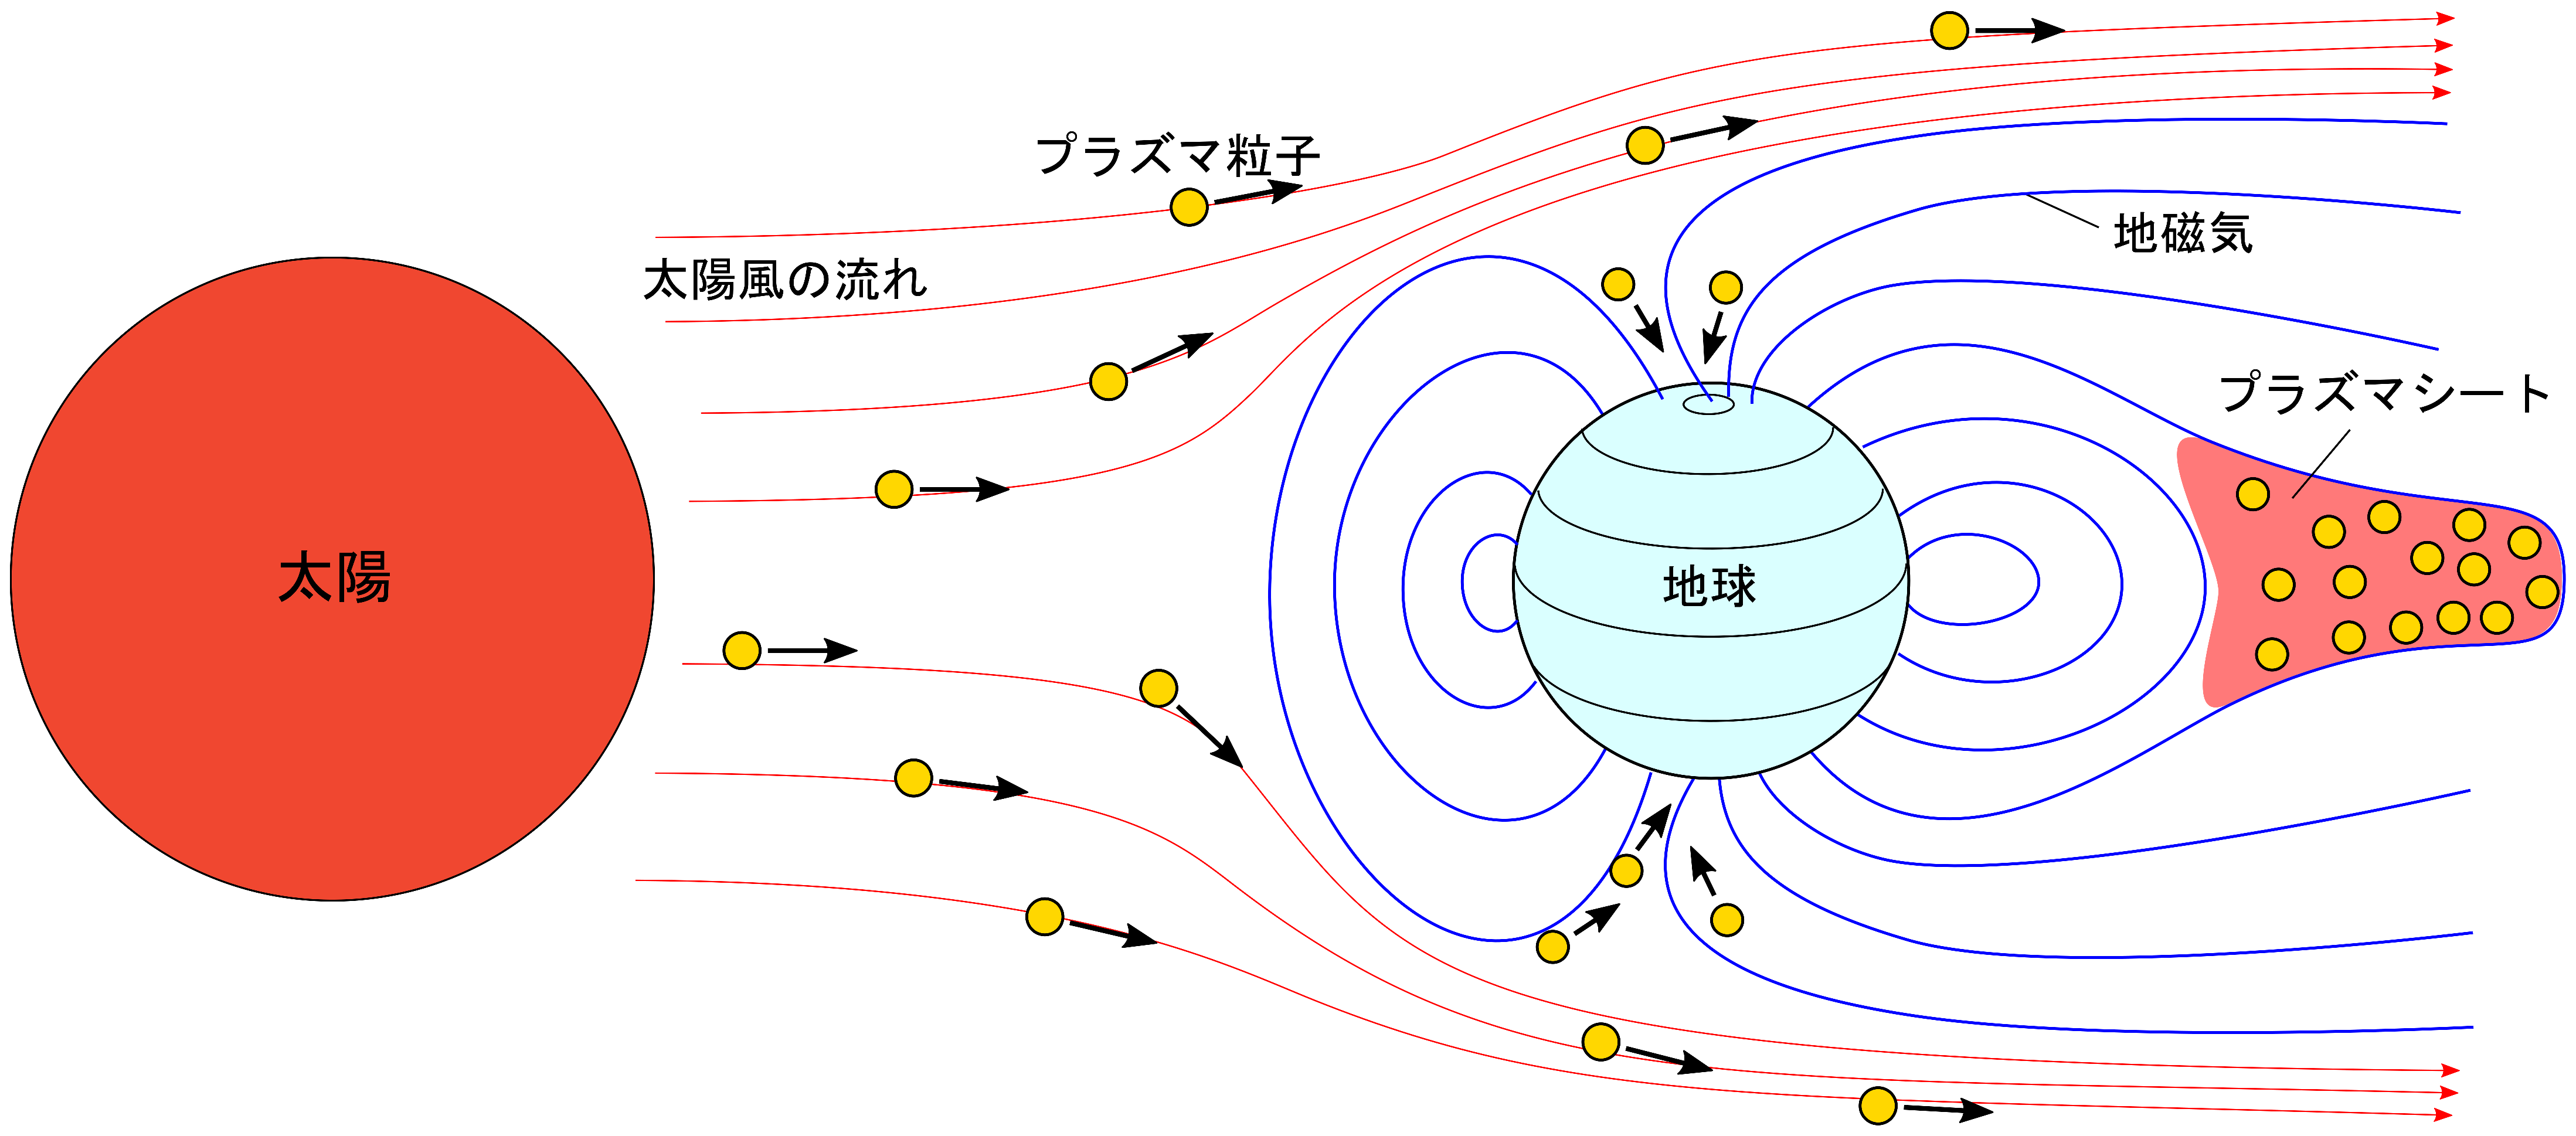
\includegraphics[width=12cm]{./chap1/eps/AuroraMechanism.eps}
  \label{fig:Mechanism1}}\\
  \subfigure[�v���Y�}���q�̋t��]{
    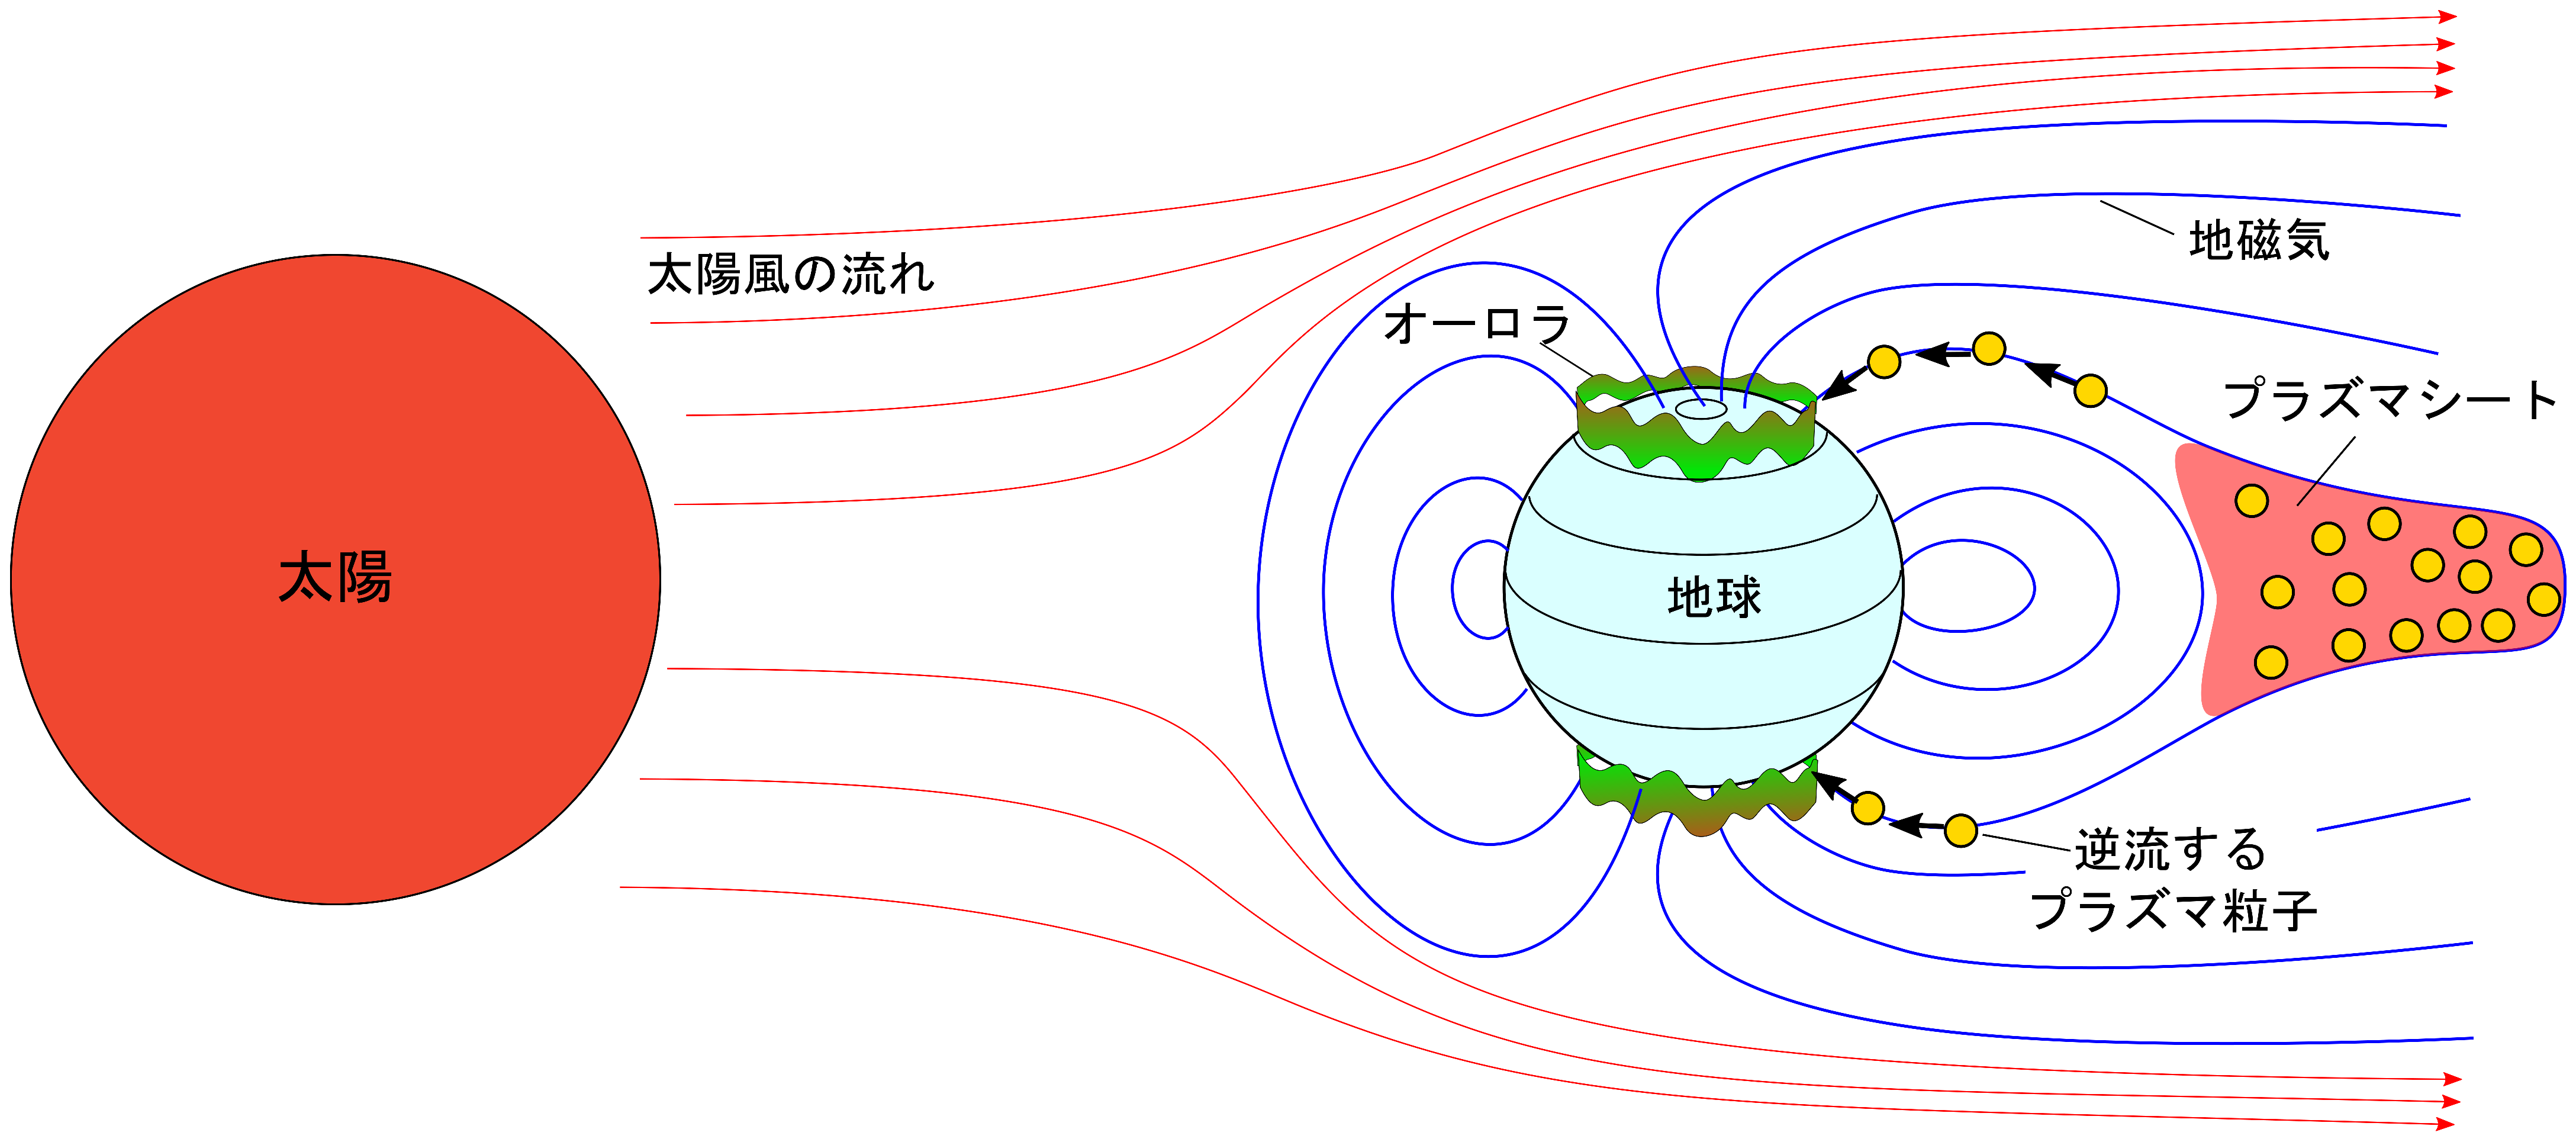
\includegraphics[width=12cm]{./chap1/eps/AuroraMechanismBreak.eps}
  \label{fig:Mechanism2}}
  \caption{�I�[�����̔������J�j�Y���T���}}
  \label{fig:Mechanism}
\end{figure}
\fi

���ݏ������Ă���I�[�����̔������J�j�Y���̊T����}\ref{fig:Mechanism}�Ɏ����D
���z�͏펞�C���z���ƌĂ΂�锜��ȃG�l���M����o���Ă���C���z���Ɋ܂܂��v���Y�}���q���₦���n���ɐ����t���Ă���D
���̃v���Y�}���q���n���ɓ��B���C��C���̕��q�ƏՓ˂��邱�ƂŔ������I�[�������`�����Ă���ƍl�����Ă���\cite{����2012}�D
�ʏ�C�n���t�߂ɓ��B�����v���Y�}���q�͒n���̎���ɎՂ��n���ɓ��B���邱�Ƃ͂Ȃ��D
�������}\ref{fig:Mechanism1}�Ɏ����悤�ɁC�v���Y�}���q�͑��z���̉e���ɂ��ό`��������̌��Ԃ��玥�C�����֐i�����C
�v���Y�}�V�[�g�ƌĂ΂��̈�ɒ~�ς����\cite{hasegawa2016}\cite{kitamura2016}�D
�����ăv���Y�}�V�[�g�ɒ~����ꂽ�v���Y�}���q�͐}\ref{fig:Mechanism2}�̂悤�ɁC���炩�̂��������ŋ}���ɉ�������Ȃ��玥�͐��ɉ����Ēn���̍��ܓx�n���ɍ~�蒍���C�I�[�����������N�����ƍl�����Ă���D
�������C�v���Y�}���q�̉������J�j�Y���̏ڍׂ͖��𖾂ł���C�n�����ӂ̉F�������w�̎�v�ȃe�[�}�ƂȂ��Ă���D\\


%\begin{figure}[t]
%\begin{center}
%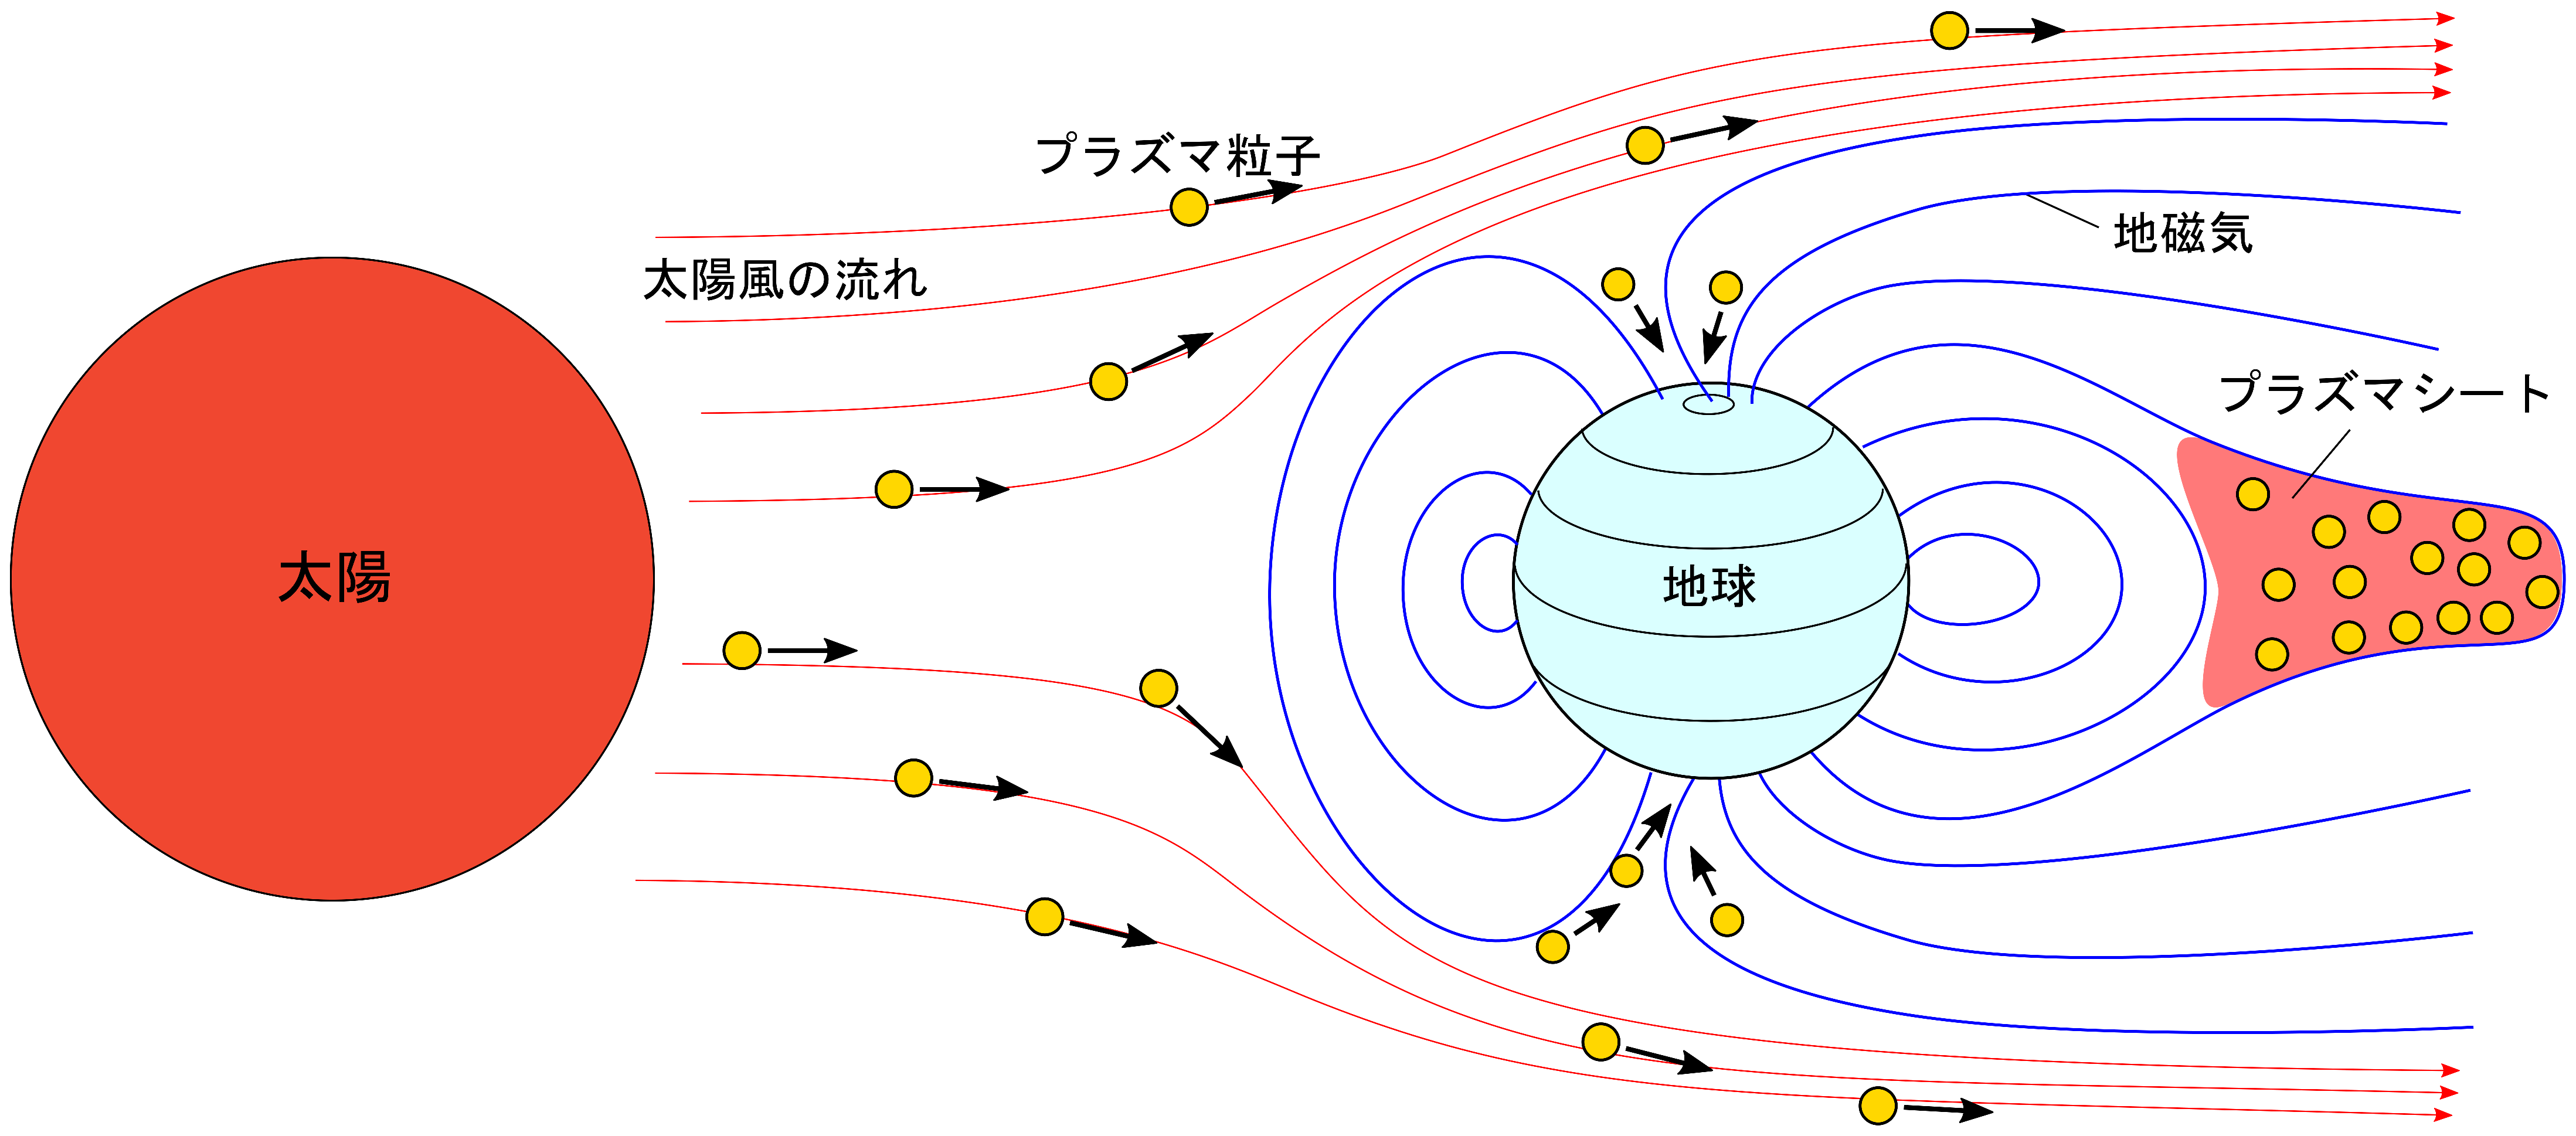
\includegraphics[width=12cm]{./chap1/eps/AuroraMechanism.eps}
%\caption{�I�[�����̔������J�j�Y���T���}}
%\label{fig:mechanism}
%\end{center}
%\end{figure}




�v���Y�}���q�̉������J�j�Y���̏ڍׂȉ𖾂́C�F�������w�ɂƂ��Ă݂̂Ȃ炸�H�w����ɂƂ��Ă����ɏd�v�Ȗ��ł���D
�v���Y�}�V�[�g�ɒ~�ς��ꂽ�v���Y�}���q����C�ɕ��o�����ہC���ɖ��邭�����ȃI�[�����������邱�Ƃ�����D
���̌��ۂ́u�I�[���������v�ƌĂ΂�C�������������ȃI�[�����̒����C�I�[�����W�F�b�g�d���ƌĂ΂��ɂ߂đ傫�ȓd��������邱�Ƃ��m���Ă���D
���̃I�[�����W�F�b�g�d���͎��ɉ�X�̐����Ɉ��e�����y�ڂ����Ƃ��񍐂���Ă���D
�Ⴆ�΁C�n��̑��d���Ɉُ�ȗU������𔭐������邱�Ƃɂ��ψ����u���[�J�[�̋@�\��Ⴢ����邱�Ƃ�����D
�܂��C�ʐM��Q�⍂�G�l���M���q�̒����ɂ��l�H�q���̌v��g���u����N���̋������񍐂���Ă���\cite{��o1999}\cite{NASA2012}�D
�d�͂�ʐM�C�l�H�q���������Ɍ������Ȃ��Ȃ��Ă��錻��ɂ����āC���̂悤�Ȉ��e����h�~���邱�Ƃ͕K�v�s�Œ��ł���D
���̂��߂ɂ̓I�[���������̈ʒu�⎞���̏����ڍׂɓ��邱�Ƃ��d�v�ł��邪�C
�O�q�̒ʂ�v���Y�}���q�̉������J�j�Y���͖����𖾂���Ă��炸�C�I�[�������������S�ɗ\�񂷂邱�Ƃ͍���ł���D
����āC�H�w�I�Ȗʂ�����v���Y�}���q�̉������J�j�Y�����𖾂��邱�Ƃ͋����]�܂�Ă���D\\


�v���Y�}���q�̉������J�j�Y���̉𖾂̂��߂ɁC�I�[������3�����`��̐��m�Ȍv�������ɗL���ł���\cite{����1994}\cite{Aurora3D}�D
�I�[�����̗��̌`��⍂�x�͒n����C�ɍ~�荞�ރv���Y�}���q�̃G�l���M���z�𔽉f���Ă���C
�I�[�����̓����̓v���Y�}���q�̓����𓊉e���Ă���D
�‚܂�C�I�[������3�����`����v�����ڍׂɒ������邱�Ƃ́C�n������̃v���Y�}���q�̋����𖾂炩�ɂ��邱�Ƃ��Ӗ����C
�������J�j�Y���̉𖾂ɂ‚Ȃ���D
�܂��C�n���ɓ��B���鑾�z���Ɋւ��錤��\cite{fujiki2014}��V�~�����[�V�����ɂ���ăv���Y�}���q�̉������J�j�Y������������\cite{ebihara2015}�������ɍs���Ă���C
�����ɑ΂����ۂɔ��������I�[�����̌v�����ʂ�g�ݍ��킹�邱�ƂŁC
�������J�j�Y���Ɋւ��闝��������ɐ[�܂�Ɗ��҂����D\\
%�ȏ�̂��Ƃ���I�[������3�����`��v���ɑ΂�����v�͍��܂��Ă���D\\

����ɃI�[������3�����`��v���́C�ߔN����オ��������Ă���3D�R���e���c�Ƃ��Ă̊��҂������D
���ۂɃA���X�J�ɂĎB�e���ꂽ�X�e���I�摜��p���āC�Ȋw�Z�p�ق̃h�[���^�v���l�^���E���u�V�����h�[���v�ł�3D���f��C
�����ɒn�������̓�ɁE�k�ɉȊw�قł̃w�b�h�}�E���g�f�B�X�v���C��p����3D�I�[�������z�̌��Ȃǂ̎��g�݂��s���Ă���D
���ۂ�3D�I�[�����f�����V�����h�[���ɏ�f����Ă���l�q��}\ref{fig:synradome}�Ɏ���\cite{�Љ�2013}�D
\\

�ȏ�̂悤�ɁC���x�̍����I�[������3�����`��v���ɑ΂�����v�͔��ɍ����D
�����āC�v���Y�}���q�̋������𖾂��邽�߂ɒ����ɂ킽�鎝���I�Ȍv�����]�܂�Ă���D
�܂��C�I�[�����͔����ꏊ�┭�������𐳊m�ɗ\�����邱�Ƃ�����Ȍ��ۂł��邱�Ƃ���C
�L�͈͂��v���”\�ȃV�X�e���ł���K�v������D
�����̂��Ƃ���C�����I�ɍL�͈͂��v���”\�ŁC���x�̍����I�[������3�����`��v�����”\�Ȏ�@�̊m�����K�v�Ƃ���Ă���D

%�ȏ�̂悤�ɁC�I�[������3�����`��v���ɑ΂�����v�͔��ɍ����D
%�������I�[�����͔����Ȕ������q�̏W���ł��邽�߁C���X���X�Ƃ��̌`��𗬓��I�ɕω������C
%�Ȃ����”������œ����I�ȃe�N�X�`���𑽂������Ȃ��Ώۂł���D
%���̂���3�����`��v���͋ɂ߂č���ł���C���m��3�����`��v���͖�����������Ă��Ȃ��D
%�����ăI�[�����̔����ꏊ�𐳊m�ɗ\�����邱�Ƃ͍���ł��邱�Ƃ���C�L�͈͂��v���”\�ȃV�X�e�����K�v�ł���D\\

%�����̂��Ƃ���C�L�͈͂��v���”\�ŁC���x�̍����I�[������3�����`��v�����”\�Ȏ�@�̊m�����K�v�Ƃ���Ă���D

\iffigure
\begin{figure}[tb]
\begin{center}
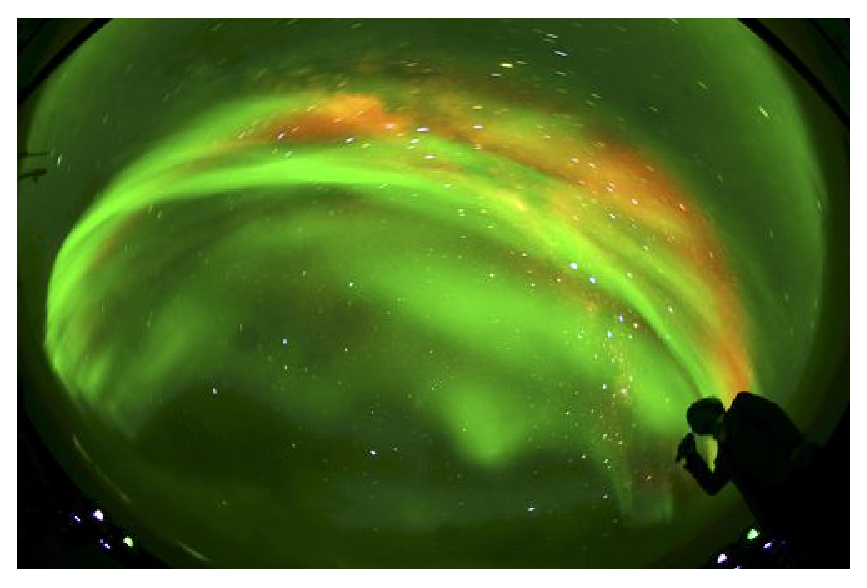
\includegraphics[width=10cm]{./chap1/eps/synradome.eps}
\caption{�V�����h�[���ŕ��f���ꂽ3D�I�[�����f��\cite{�Љ�2013}}
\label{fig:synradome}
\end{center}
\end{figure}
\fi

\clearpage
%%%%%%%%%%%%%%%%%%%%%%%%%%%%%%%%%%%%%%%%%%%%%%%%%%%%%%%%%%%%%%%%%%%%%%%%%%%%%%%%%%%%%%%%%%%%%%%%%%%%%%%%%%%%%%%%%%%%%%%%%%%%%%%%%%%
\section{�I�[������3�����v���Ɋւ���]������}
\label{sec:related_research}
�I�[������3���v�������݂錤���͂���܂łɂ��������s���Ă����D
�{�߂ł͂����̌����Ɋւ��ďq�ׂ�ƂƂ��ɁC���ꂼ��̌����̎��–��_���q�ׁC
�{�����̏d�v���ƈʒu�t���𖾊m�ɂ���D

\subsection{�I�[�����̕����I�ȍ��x�v��}


St\"ormer��1913�N����1915�N�ɂ����āC�m���E�F�[�ɐݒu����2��̃J��������擾���ꂽ�摜�΂�p���āC�I�[�����̈ꕔ�̍��x���v������\cite{stormer1915}�D
�蓮�ɂ��摜�΂���Ή��_�����߂邱�ƂŃX�e���I�v���ɂ���ăI�[�����̑�܂��ȍ��x�𐄒肵���D
�}\ref{fig:stormer_stereo}��St\"ormer���g�p�����I�[�����̉摜�΂��C�}\ref{fig:stormer_result}�Ɏ蓮�ɂ��Ή��_���o�̌��ʂ������D
�}\ref{fig:stormer}���番����ʂ�C�I�[�����摜�͓����̏��Ȃ��摜�̂���
������Ή��_�͏��Ȃ��C���Ɍ��肳�ꂽ�����̍��x�������肷�邱�Ƃ��ł��Ȃ������D\\
%�X�Ɏ蓮�ɂ���đΉ��_�����o���Ă��邽�߁C������f�[�^�ʂɌ��E���������D\\

\iffigure
\begin{figure}[b]
  \centering
  \subfigure[�X�e���I�摜��]{
    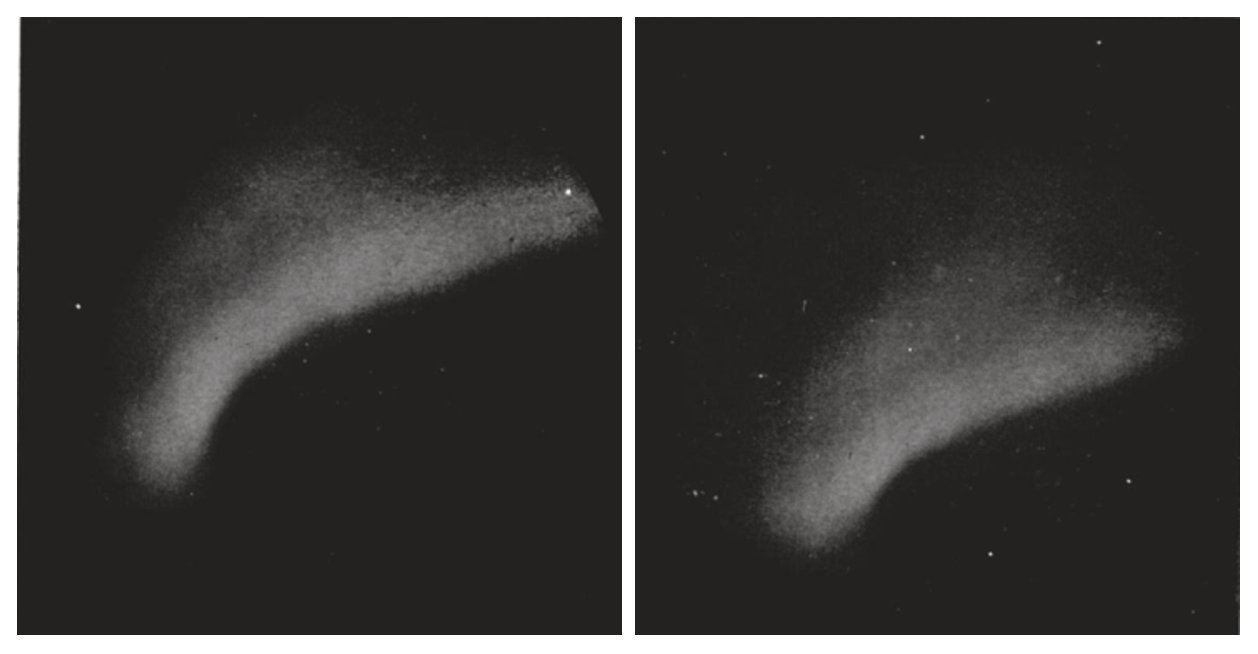
\includegraphics[width=8cm]{./chap1/eps/stormer_stereo.eps}
  \label{fig:stormer_stereo}}
  \subfigure[�X�e���I�v������]{
    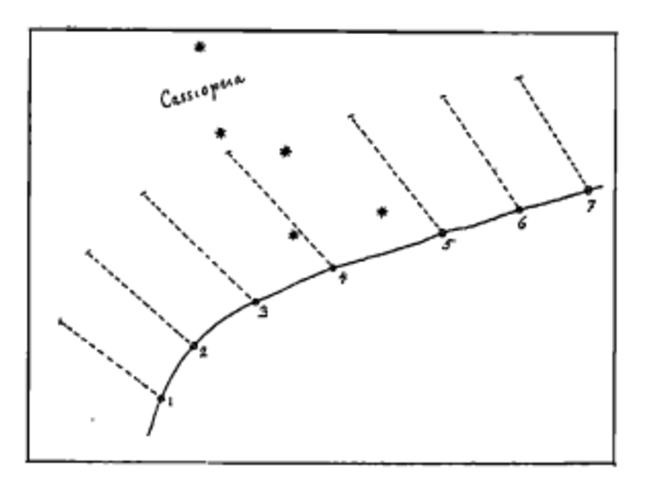
\includegraphics[width=4cm]{./chap1/eps/stormer_result.eps}
  \label{fig:stormer_result}}
  \caption{St\"ormer�ɂ��v��\cite{stormer1915}}
  \label{fig:stormer}
\end{figure}
\fi

���̌�CBrown��̓A���X�J�ɐݒu����2��̃J�����ɂ����St\"ormer���l�X�e���I�v�����s���C
�����I�[�����ƌĂ΂��10�b�O��̎����Ŗ��ł��J��Ԃ��I�[�����̃G�b�W�ɒ��ڂ����v����@���Ă���\cite{brown1976}�D
�����I�[�����̉摜�΂���G�b�W�𒊏o���C���o���ꂽ�G�b�W�`����r���邱�ƂőΉ��_���o���s���C�I�[�����̉��[�̍��x�𐄒肵���D
�}\ref{fig:brown}��Brown�炪�I�[�����摜����G�b�W�𒊏o�������ʂ������D
�������C���̎�@�ɂ����Ă��I�[�����摜���̃G�b�W�����̍��x�������肷�邱�Ƃ��ł����C
�I�[�����S�̂̌v�����s�����Ƃ͂ł��Ȃ������D
�܂��CSt\"ormer�̎�@�ɂ����Ă�Brown��̎�@�ɂ����Ă��C�g�p���ꂽ�J�����̃L�����u���[�V�����������łȂ����m���Ɍ�������@�ł������D\\

\iffigure
\begin{figure}[tb]
\begin{center}
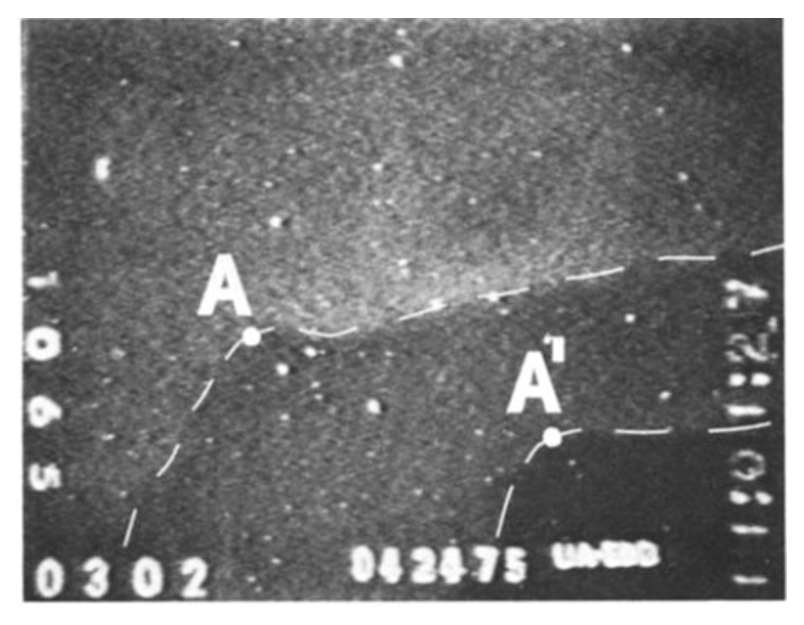
\includegraphics[width=8cm]{./chap1/eps/brown1976.eps}
\caption{Brown�ɂ��v��\cite{brown1976}}
\label{fig:brown}
\end{center}
\end{figure}
\fi




\subsection{�g���O���t�B�ɂ��3�����`��v��}

�Z�p�̐i���ɔ����C�I�[�����̕����I��3�����v���ł͂Ȃ��I�[�����S�̂�3�����`����v�������@����Ă���Ă����D
���̂悤�Ȍ����ɁC�g���O���t�B�Z�p�𗘗p�����I�[�����v��������D
�g���O���t�B�Ƃ͒f�w�e���@�Ƃ��Ă΂�CX��CT�iComputed Tomography�j�̂悤�Ȉ�Ðf�f���ɂ��p�����Ă���t��͋Z�p�ł���D
��ʓI�ɂ́C�����Ώۗ̈�����͂ނ悤�ɐ����⌟�o�킪�z�u����C
���o��̃f�[�^���č\�����邱�ƂőΏۂ̓����\�����擾�����D\\
%2��̃J������p�����X�e���I�v���ɂ��I�[�����v���݂̂łȂ��C�g���O���t�B�Z�p�����p�����I�[�����v�����s���Ă����D

Aso���1990�N��2��̃J�����ɂ���Ď擾����2�����摜����C�g���O���t�B�Z�p��p���ăI�[������3�����`����č\�������@���Ă���\cite{aso1990}�D
���̎�@�ł̓g���O���t�B���s���ɂ͊ϑ��_�����Ȃ����Ƃ���C�I�[�����̔����`����֐��Ń��f�������C����`�ŏ����@�ɂ���ă��f���p�����[�^�𐄒肵���D
��������͂�2�n�_����݂̂̓��͉摜�ł̓I�[�����̍\���𕜌�����ɂ͏\���ł͂Ȃ������D\\

����ɑ΂��C���̌�Aso���Tanaka��͕�����̃J�����╨���ʑ�����n��ɐݒu���邱�ƂŁC�I�[�����̃g���O���t�B��͂��s����\cite{aso1998}\cite{tanaka2011}�D
Tanaka��̌����ɂ����Ďg�p���ꂽ�@��̈ʒu��}\ref{fig:TomographyCameras}�Ɏ����D
�}\ref{fig:TomographyCameras}���̐F�̎O�p�͐ݒu���ꂽ�J�����������Ă���D�܂��C�ԐF�̕H�`��EISCAT���[�_�ƌĂ΂��d�q���x�����v�����鑕�u�̈ʒu�C�ΐF�̎l�p�͉F�����瓞�B����d�g�G�����v�����邽�߂�IRIS�ƌĂ΂�鑕�u�̈ʒu�������Ă���D
������p���邱�ƂŃg���O���t�B��͂ɂ��I�[������3�����`��v�����”\�ɂȂ������C
���̌����ɂ����ăI�[�������v���ł���͈͂͐}\ref{fig:TomographyCameras}���̋Ȑ����\������Ă���̈�݂̂ł���C
�@��̐��ɑ΂��Ĕ��Ɍ���ꂽ�͈͂����v���ł��Ȃ������D
���̂��ߍL�͈͂��v������ړI�ɂ͕s�����Ȏ�@�ł������D

\iffigure
\begin{figure}[tb]
\begin{center}
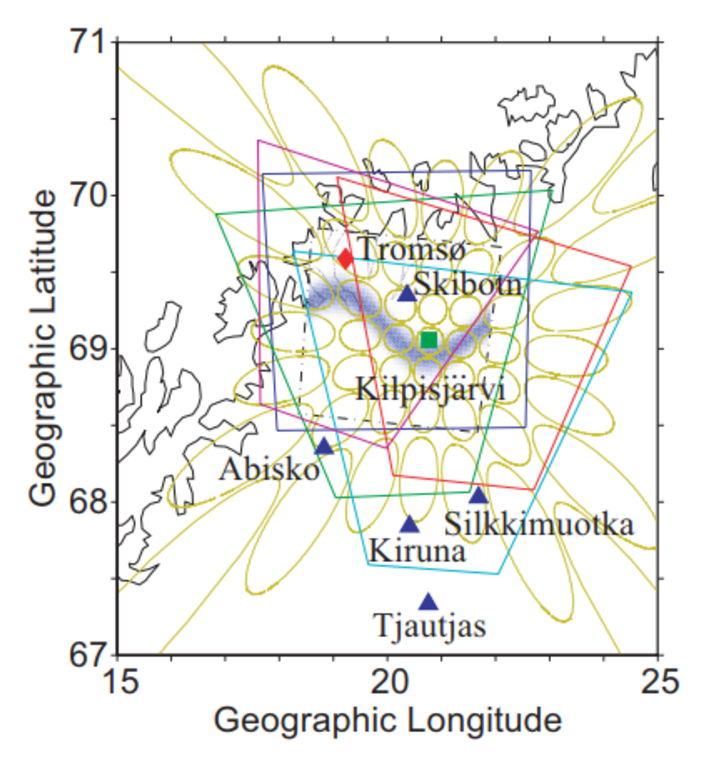
\includegraphics[width=8cm]{./chap1/eps/TomographyCameras.eps}
\caption{Tanaka��̎�@�ɂ�����@��̐ݒu�ʒu\cite{tanaka2011}}
\label{fig:TomographyCameras}
\end{center}
\end{figure}
\fi



\subsection{�n��ƉF������̌v��}
�lj��\��
%�ߔN�ł́C�n��ɐݒu�����@��ɉ����F����Ԃɂ���@���p���ăI�[�������v�����錤��������ɍs���Ă���D
%Sharp�̓��P�b�g�Ɍv��𓋍ڂ��邱�ƂŁC
%�I�[�������`�����Ă�����̂�������̔g���̌��̕��o���x�ƍ��x�̊֌W���F����Ԃ��璼�ڌv������\cite{sharp1971}�D
%�܂��CNishimura���Samara��͐l�H�q���ɓ��ڂ��ꂽ�v��̏���p���āC�n��ɐݒu�����J�����ŎB�e�����I�[������
%�v���Y�}���q�̃G�l���M�̑傫�����֌W�Â����D






\subsection{�n��ɐݒu��������X�e���I�J�����ɂ��3�����`��v��}
��L�̖����������邽�߂ɁC�����ɃL�����u���[�V�������ꂽ2��̋���J������p���ăI�[�����S�̂�3�����`����v�����錤�����Ȃ���Ă���\cite{kataoka2013}\cite{�v��2013}\cite{fujii2014}\cite{�|��2015}�D
%�n��ɐݒu����2��̋���J������
%����I�[������3�����`����v�������@������\cite{�v��2013}\cite{fujii2014}�D
%Kataoka���v�ۂ��Fujii��̓A���X�J�ɐݒu����2��̋���J��������I�[������3�����`����v�������@���Ă���\cite{�v��2013}\cite{fujii2014}�D
���̎�@�ł�2��̋���J�������g�p���C�������ɎB�e��������摜�΂���͂Ƃ����X�e���I�v�����s���Ă���D
����ɂ���ċ@��ɑ΂��Ĕ��ɍL�͈͂̌v�����”\�ƂȂ����D
�����Đ��x�̍����L�����u���[�V������@��K�p���邱�ƂŁC�v���̐M������ۏ؂����D\\


\begin{figure}[htb]
  \centering
  \subfigure[�f�B�X�N���[�g�I�[�����̍��x���茋��]{
    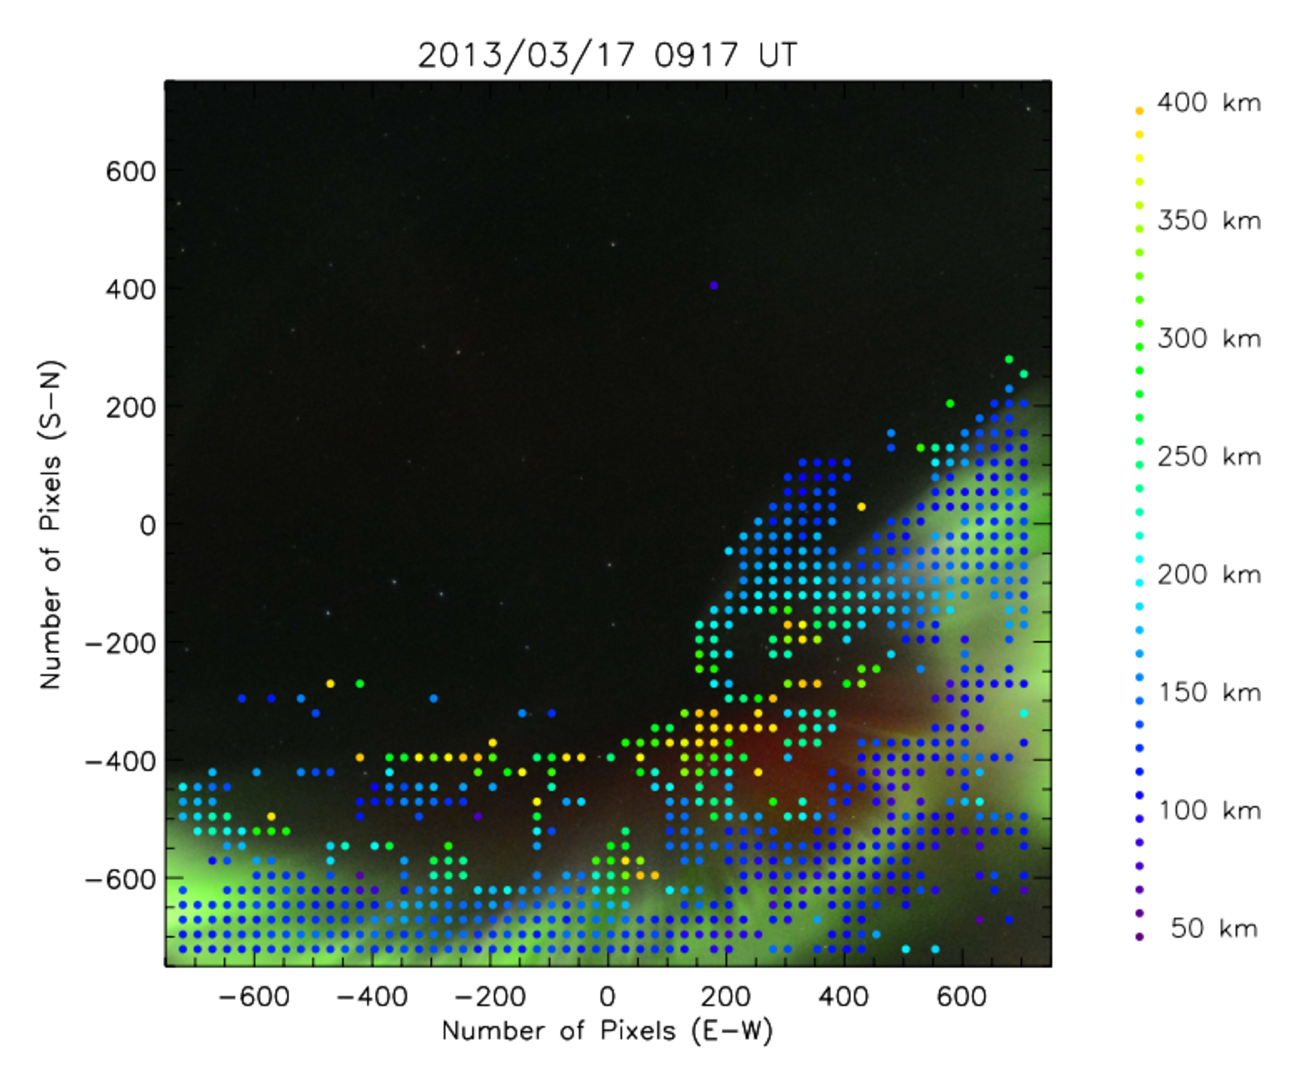
\includegraphics[width=9cm]{./chap1/eps/Kataoka1.eps}
  \label{fig:kataoka2013_1}}
  \subfigure[�����I�[�����̍��x���茋��]{
    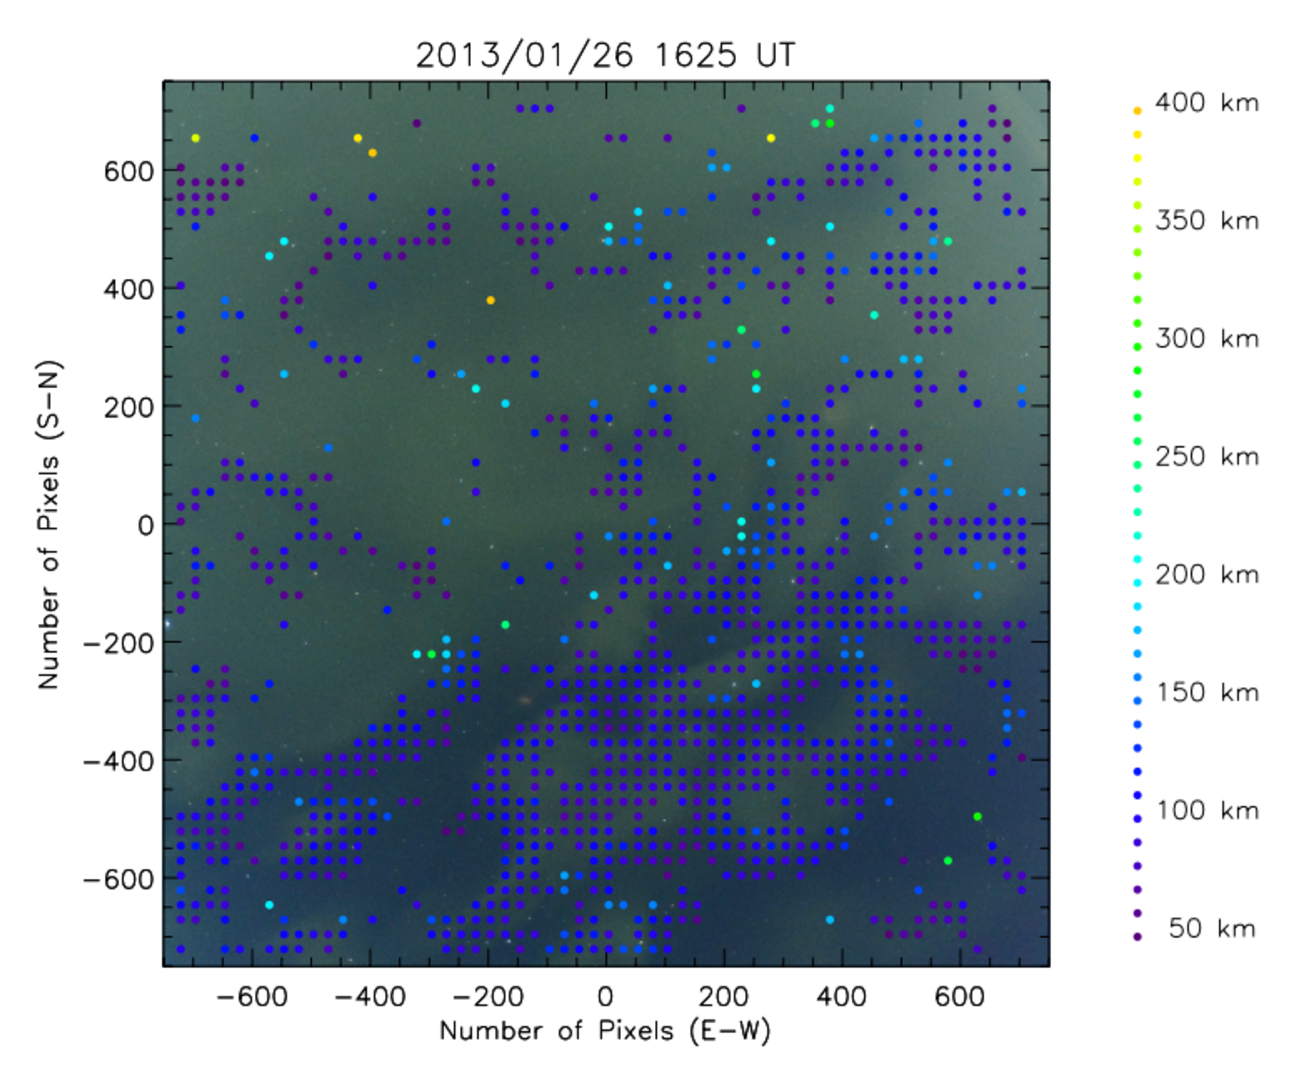
\includegraphics[width=9cm]{./chap1/eps/Kataoka2.eps}
  \label{fig:kataoka2013_2}}
  \caption{Kataoka��ɂ�鍂�x���茋��\cite{kataoka2013}}
  \label{fig:kataoka2013}
\end{figure}


�I�[�����̕����I�ȍ��x����ɂƂǂ܂���St\"ormer��Brown��̌����ɑ΂��āC
Kataoka��͉摜���ɑ��݂���I�[�����S�̂̍��x������s����\cite{kataoka2013}�D
���̎�@�ł͋���X�e���I�J�����ŎB�e�����摜�΂��ו������C�ו������ꂽ���̈�̍��x���v���[���X�C�[�v�@�ɂ���Đ��肵���D
��̓I�ɂ́C�܂�����̋���J�����摜���̏��̈悪���鍂�x�ɑ��݂���Ɖ��肵�C�����̃J�����摜���̑Ή����鏬�̈���Z�o�����̂��ɏ��̈擯�m�̗ގ��x��]������D
�����č��x�̉���Ɨގ��x�̕]�����J��Ԃ��C�ł��ގ��x�̍������x�����̈�̍��x�ł���Ɛ��肵���D
Kataoka��ɂ��I�[�����̍��x����̌��ʂ�}\ref{fig:kataoka2013}�Ɏ����D
�}\ref{fig:kataoka2013_1}�̓f�B�X�N���[�g�I�[�����ƌĂ΂��C�J�[�e����̂͂����肵���I�[�����̍��x���茋�ʁC
�}\ref{fig:kataoka2013_2}�͖����I�[�����̍��x���茋�ʂł���D
���������̎�@�́C�摜�̑S�̈�Ɋւ��ď������s���Ă���C�I�[�����̈�݂̂ɑ΂��č��x������s�������̂ł͂Ȃ������D
���̂��߂��̎�@�́C�摜���̃I�[�����̂����悻�̍��x���z���m�F���邽�߂ɂ͔��ɗL���ł��������C
����ꂽ���ʂ��I�[�����݂̂̐��m�Ȍ`�󕜌��ɗ��p���邱�Ƃ͍���ł������D\\





�v�ۂ��Fujii��́C����X�e���I�摜�΂���I�[�����̈�𒊏o��SIFT��p���đΉ��_�����o���邱�ƂŁC
�I�[�����S�̂�3�����`��̌v���ɐ�������\cite{�v��2013}\cite{fujii2014}�D
�܂��C����ꂽ�Ή��_�Q��3�p�`���b�V����\�邱�Ƃ�3�����`��𕜌������D
Fujii��̎�@�ɂ��Ή��_���o���ʂ�}\ref{fig:Fujii_result_intro}�Ɏ����D
���E�̃I�[�����摜���猟�o���ꂽ�Ή��_��ԐF�̓_�Ńv���b�g���Ă���D
�}\ref{fig:Fujii_result_intro}���番����ʂ�C���̎�@�ł̓I�[�����̈�ɑ΂��ē�����Ή��_�����ɏ��Ȃ��C
���x���Ⴂ�Ƃ�����肪�������D\\




\clearpage


\begin{figure}[tb]
\begin{center}
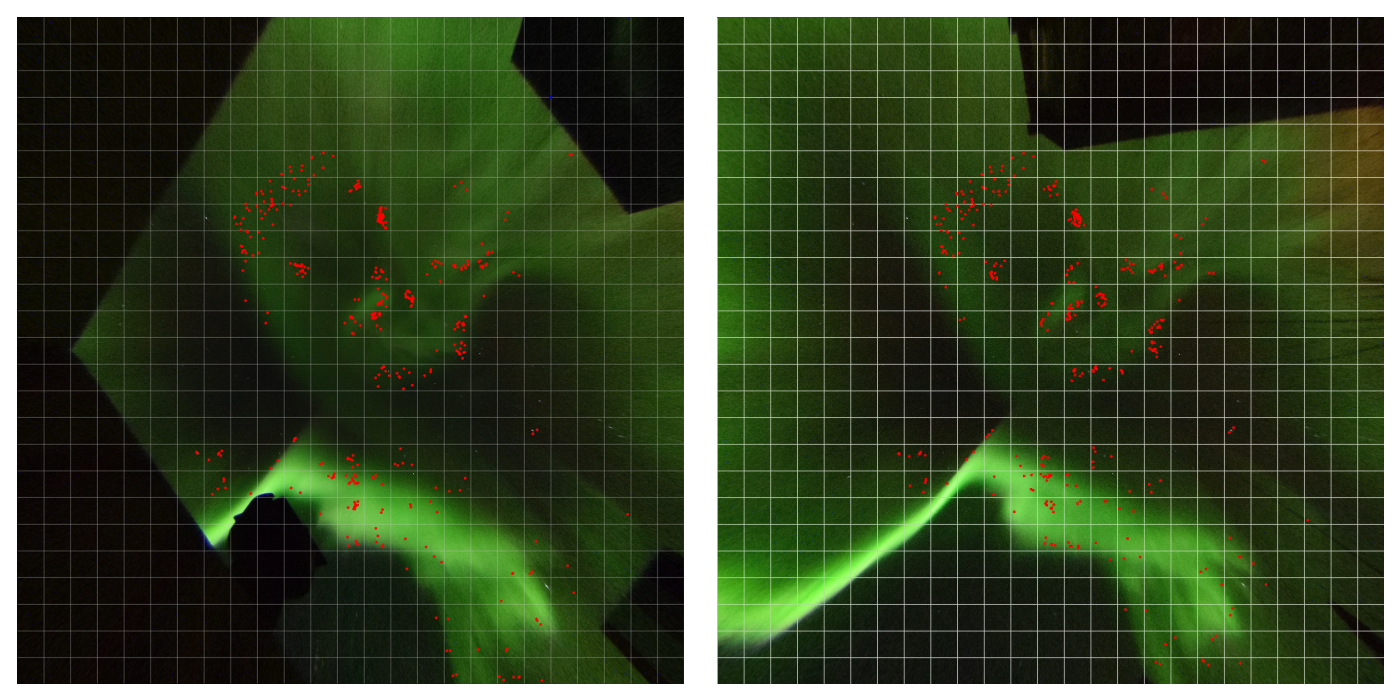
\includegraphics[width=11cm]{./chap1/eps/014_Kubo.eps}
\caption{Fujii��̎�@\cite{fujii2014}�ɂ��Ή��_���o����}
\label{fig:Fujii_result_intro}
\end{center}
\end{figure}

\begin{figure}[htb]
\begin{center}
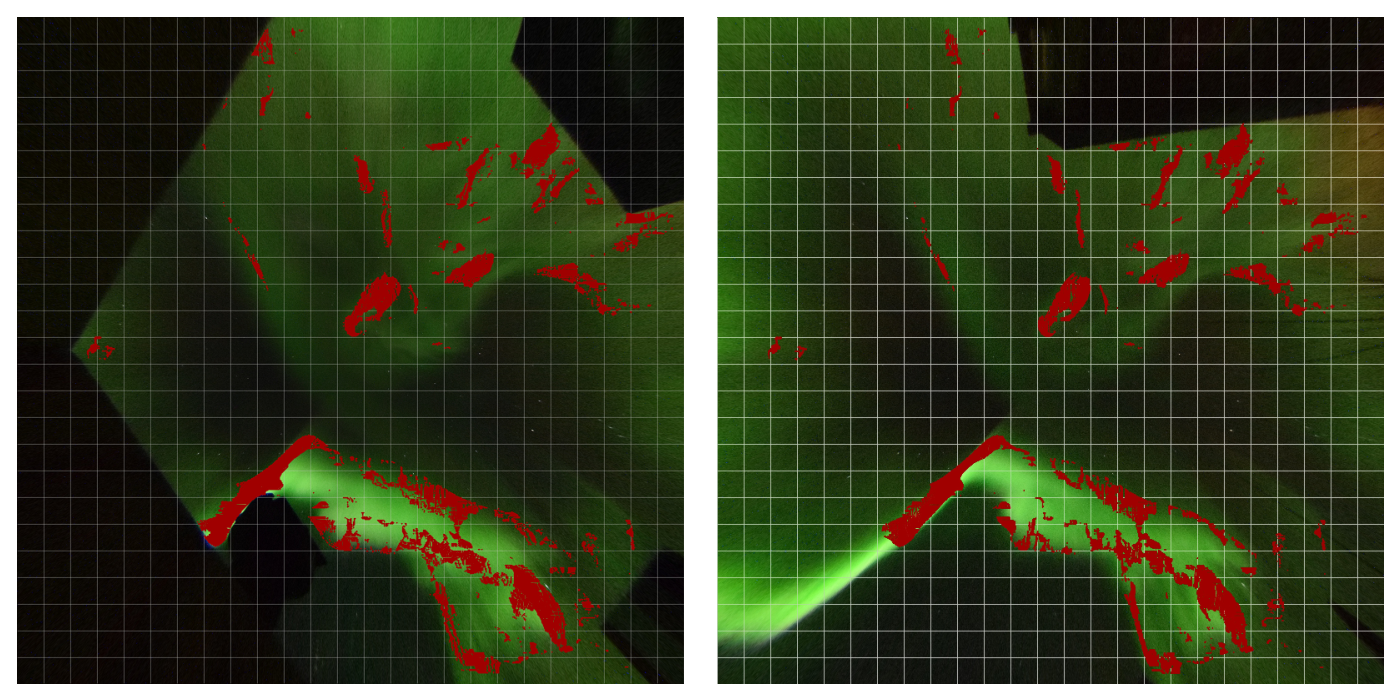
\includegraphics[width=11cm]{./chap1/eps/014_takeuchi_b4.eps}
\caption{Takeuchi��̎�@\cite{�|��2015}�ɂ��Ή��_���o����}
\label{fig:Takeuchi_result_intro}
\end{center}
\end{figure}
%\clearpage

����ɑ΂��|����́C�e���v���[�g�}�b�`���O�ɂ���đΉ��_�����o���C������Ή��_�𑝉��������D
�܂��C�Ή��_�����ԕ����֒ǐՂ��邱�ƂŐ��x�����コ����\cite{�|��2015}�D
�}\ref{fig:Fujii_result_intro}�Ɠ����摜�΂ɑ΂��Ē|����̑Ή��_���o��@��K�p�������ʂ�}\ref{fig:Takeuchi_result_intro}�Ɏ����D
�}\ref{fig:Fujii_result_intro}���l�ɁC���o���ꂽ�Ή��_��ԐF�̓_�Ńv���b�g���Ă���D
%�}\ref{fig:Takeuchi_result_intro}���番����悤�ɁC���o�����Ή��_���𑝉������C���̐��x�����コ������
�������C�}\ref{fig:Fujii_compare}�Ɏ����悤�ɁC�|����̎�@�ɂ���ĕ��������I�[������3�����`�󌋉ʂ���́C���ۂ̃I�[�����Ɍ�����悤�Ȋ��炩�ȃJ�[�e���`��͌����Ȃ������D
�I�[�����摜�͓����I�ȃe�N�X�`�������ɏ��Ȃ��ɂ�������炸�C
�Ή��_���o���摜���݂̂�p���čs���Ă��邱�Ƃ���C
�Ή��_�����o����Ȃ��I�[�����̈悪�傫���C����ɓ����I�ȃe�N�X�`���ȊO�̗̈�ł̑Ή��_���o�ɂ����ď\���Ȑ��x�������Ȃ��������Ƃ������ƍl������D\\


�����܂ŁC����܂łɍs���Ă����I�[������3�����`��v���̌����ɂ‚��ďq�ׂ��D
�������C�L�͈͂��v���”\�ŁC�Ȃ������x�̍����v����@�͖�����Ă���Ă��Ȃ��D
�@��ɑ΂��čL�͈͂̌v�����s�����߂ɂ͋���X�e���I�J������p�����v�����L���ł������C
�v�����x�͂���Ȃ���オ���߂��Ă���D
�����𓥂܂��C���߂ł͖{�����̖ړI�ɂ‚��ďq�ׂ�D
%�����Ŗ{�����ł́C�L�͈͂��v�����邽�߂ɁC�n��ɐݒu��������J�����ɂ��擾����摜��p����3�����v�����s���D
%�����Đ��x�̍����v�����ʂ𓾂邽�߂ɁC�I�[�����摜�Β��̃I�[�����̈�̑S�悩�疧�ō����x�ȑΉ��_���o���”\�ɂ����@���\�z����K�v������D

\iffigure
\begin{figure}[b]
  \centering
  \subfigure[�|����̎�@�ɂ��I�[����3�����`�󕜌�����]{
    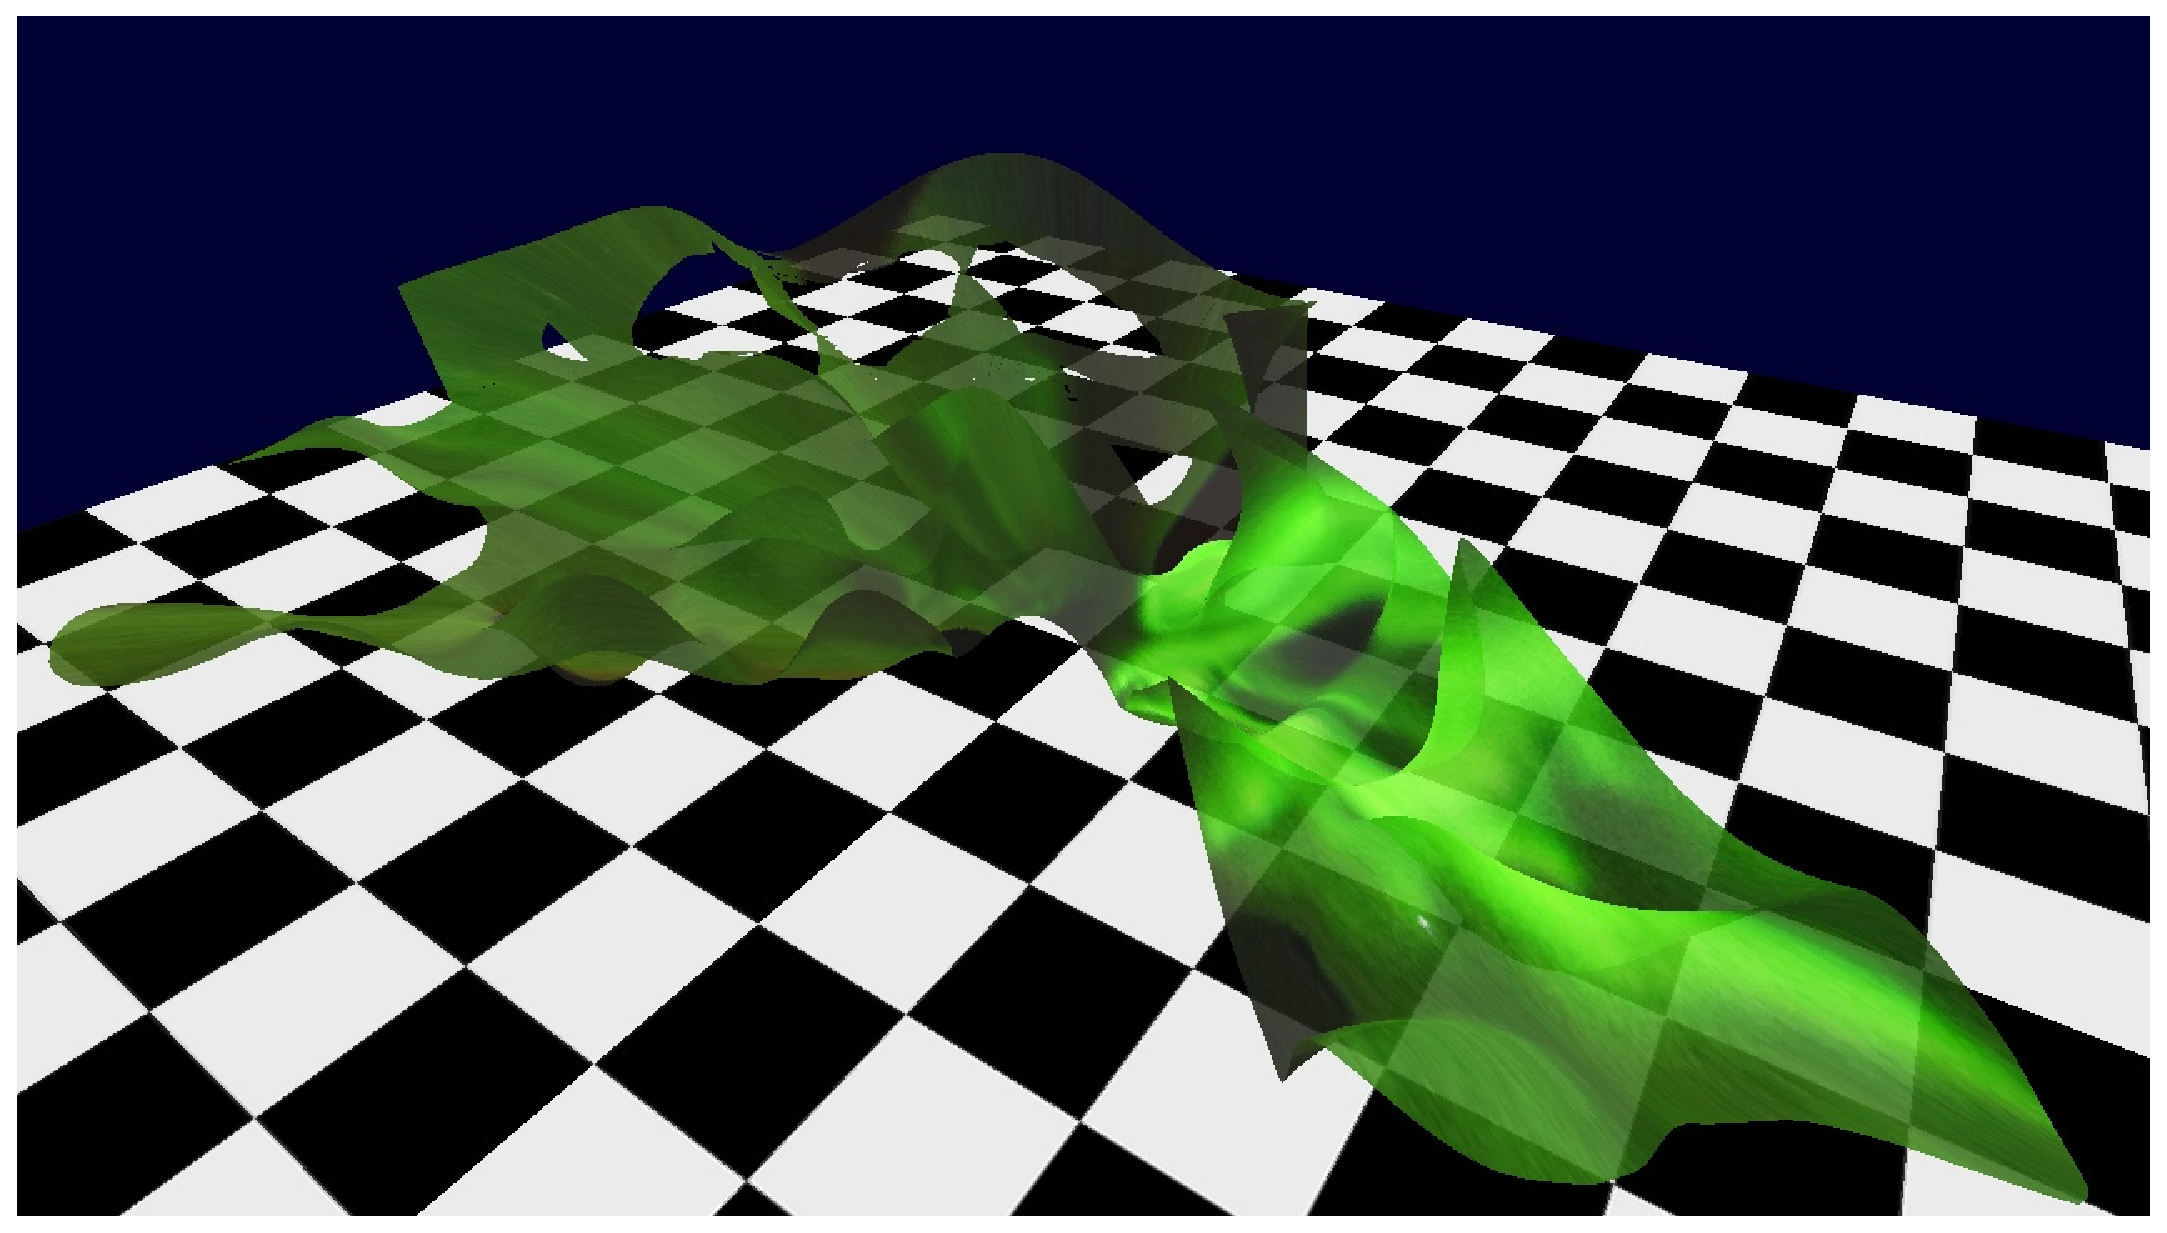
\includegraphics[width=10cm]{./chap1/eps/Shape_takeuchi_b4.eps}
  \label{fig:fujii_result}}\\
  \subfigure[�J�[�e����̃I�[�����̗�]{
    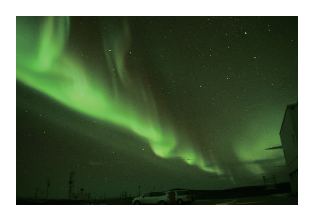
\includegraphics[width=10cm]{./chap1/eps/Aurora_curtain.eps}
  \label{fig:aurora_curtain}}
  \caption{�|����̎�@\cite{�|��2015}�ɂ��I�[����3�����`�󕜌����ʂƎ��ۂ̃I�[�����`��̔�r}
  \label{fig:Fujii_compare}
\end{figure}
\fi

\clearpage
%%%%%%%%%%%%%%%%%%%%%%%%%%%%%%%%%%%%%%%%%%%%%%%%%%%%%%%%%%%%%%%%%%%%%%%%%%%%%%%%%%%%%%%%%%%%%%%%%%%%%%%%%%%%%%%%%%%%%%%%%%%%%%%%%%%
\section{�����̖ړI}
\label{sec:objective}

\ref{sec:background}�߂ɂ����āC�I�[������3�����`����L�͈͂ɂ킽�萳�m�Ɍv���”\�Ȏ�@�̊m�����K�v�Ƃ���Ă��邱�Ƃ��q�ׂ��D
�܂�\ref{sec:related_research}�߂��C�@��ɑ΂��čL�͈͂̌v�����s�����߂ɂ͋���X�e���I�J������p�����v�����L���ł������C
����X�e���I�J������p���������x�ȃI�[������3�����v���ƉŽ������”\�Ȏ�@�͂܂��m������Ă��Ȃ����Ƃ����炩�ƂȂ����D\\
%�L�͈͂��ϑ��”\�ł���C�Ȃ������x�̍���3�����v�����”\�Ȏ�@�͂܂��m������Ă��Ȃ��D
%���x�̍���3�����v���̂��߂ɂ́C���ō����x�ȑΉ��_���o�����߂���D

�����ŁC�{�����̖ړI���ȉ��̂悤�ɐݒ肷��D
\begin{center}
\doublebox{
\begin{tabular}{c}
����X�e���I�J������p����\\
�����x�ȃI�[������3�����`��v���ƉŽ����̎���
\end{tabular}
}
\end{center}



\textcolor{red}{�Ž����ɂ‚��Č��y����}


\clearpage
%%%%%%%%%%%%%%%%%%%%%%%%%%%%%%%%%%%%%%%%%%%%%%%%%%%%%%%%%%%%%%%%%%%%%%%%%%%%%%%%%%%%%%%%%%%%%%%%%%%%%%%%%%%%%%%%%%%%%%%%%%%%%%%%%%%
%\section{�����̃A�v���[�`}
%\label{sec:approach}

%\clearpage

%%%%%%%%%%%%%%%%%%%%%%%%%%%%%%%%%%%%%%%%%%%%%%%%%%%%%%%%%%%%%%%%%%%%%%%%%%%%%%%%%%%%%%%%%%%%%%%%%%%%%%%%%%%%%%%%%%%%%%%%%%%%%%%%%%%
\section{�{�_���̍\��}

�{�_���͑S7�͂���\������Ă���D�{�_���̍\����}\ref{fig:Thesis_flow}�Ɏ����D

��1�͂ł́C�{�����̔w�i�ƖړI�C�A�v���[�`�ɂ‚��ďq�ׂ��D

��2�͂ł́C�{�����̃A�v���[�`�ɂ‚��ďq�ׂ�D

��3�͂ł́C�{��Ď�@���s�����߂ɕK�v�ȁC�I�[�����摜�ɑ΂��鏈���ɂ‚��ďq�ׂ�D

��4�͂ł́C����J������p���ĎB�e���ꂽ�I�[�����摜�΂���̖��ō����x�ȑΉ��_���o��@�ƁC�I�[������3�����Ž�����@�ɂ‚��ďq�ׂ�D

��5�͂ł́C�{��Ď�@�̗L���������؂��邽�߂ɍs�����V�~�����[�V���������ɂ‚��ďq�ׂ�D

��6�͂ł́C�{��Ď�@�̗L���������؂��邽�߂ɃA���X�J�ōs���������ɂ‚��ďq�ׂ�D

��7�͂ł́C�{�����Ɋւ��錋�_�ƍ���̓W�]���q�ׂ�D

\textcolor{red}{�Ō�܂ŏ���������������ڂ�������}

\begin{figure}[tb]
\begin{center}
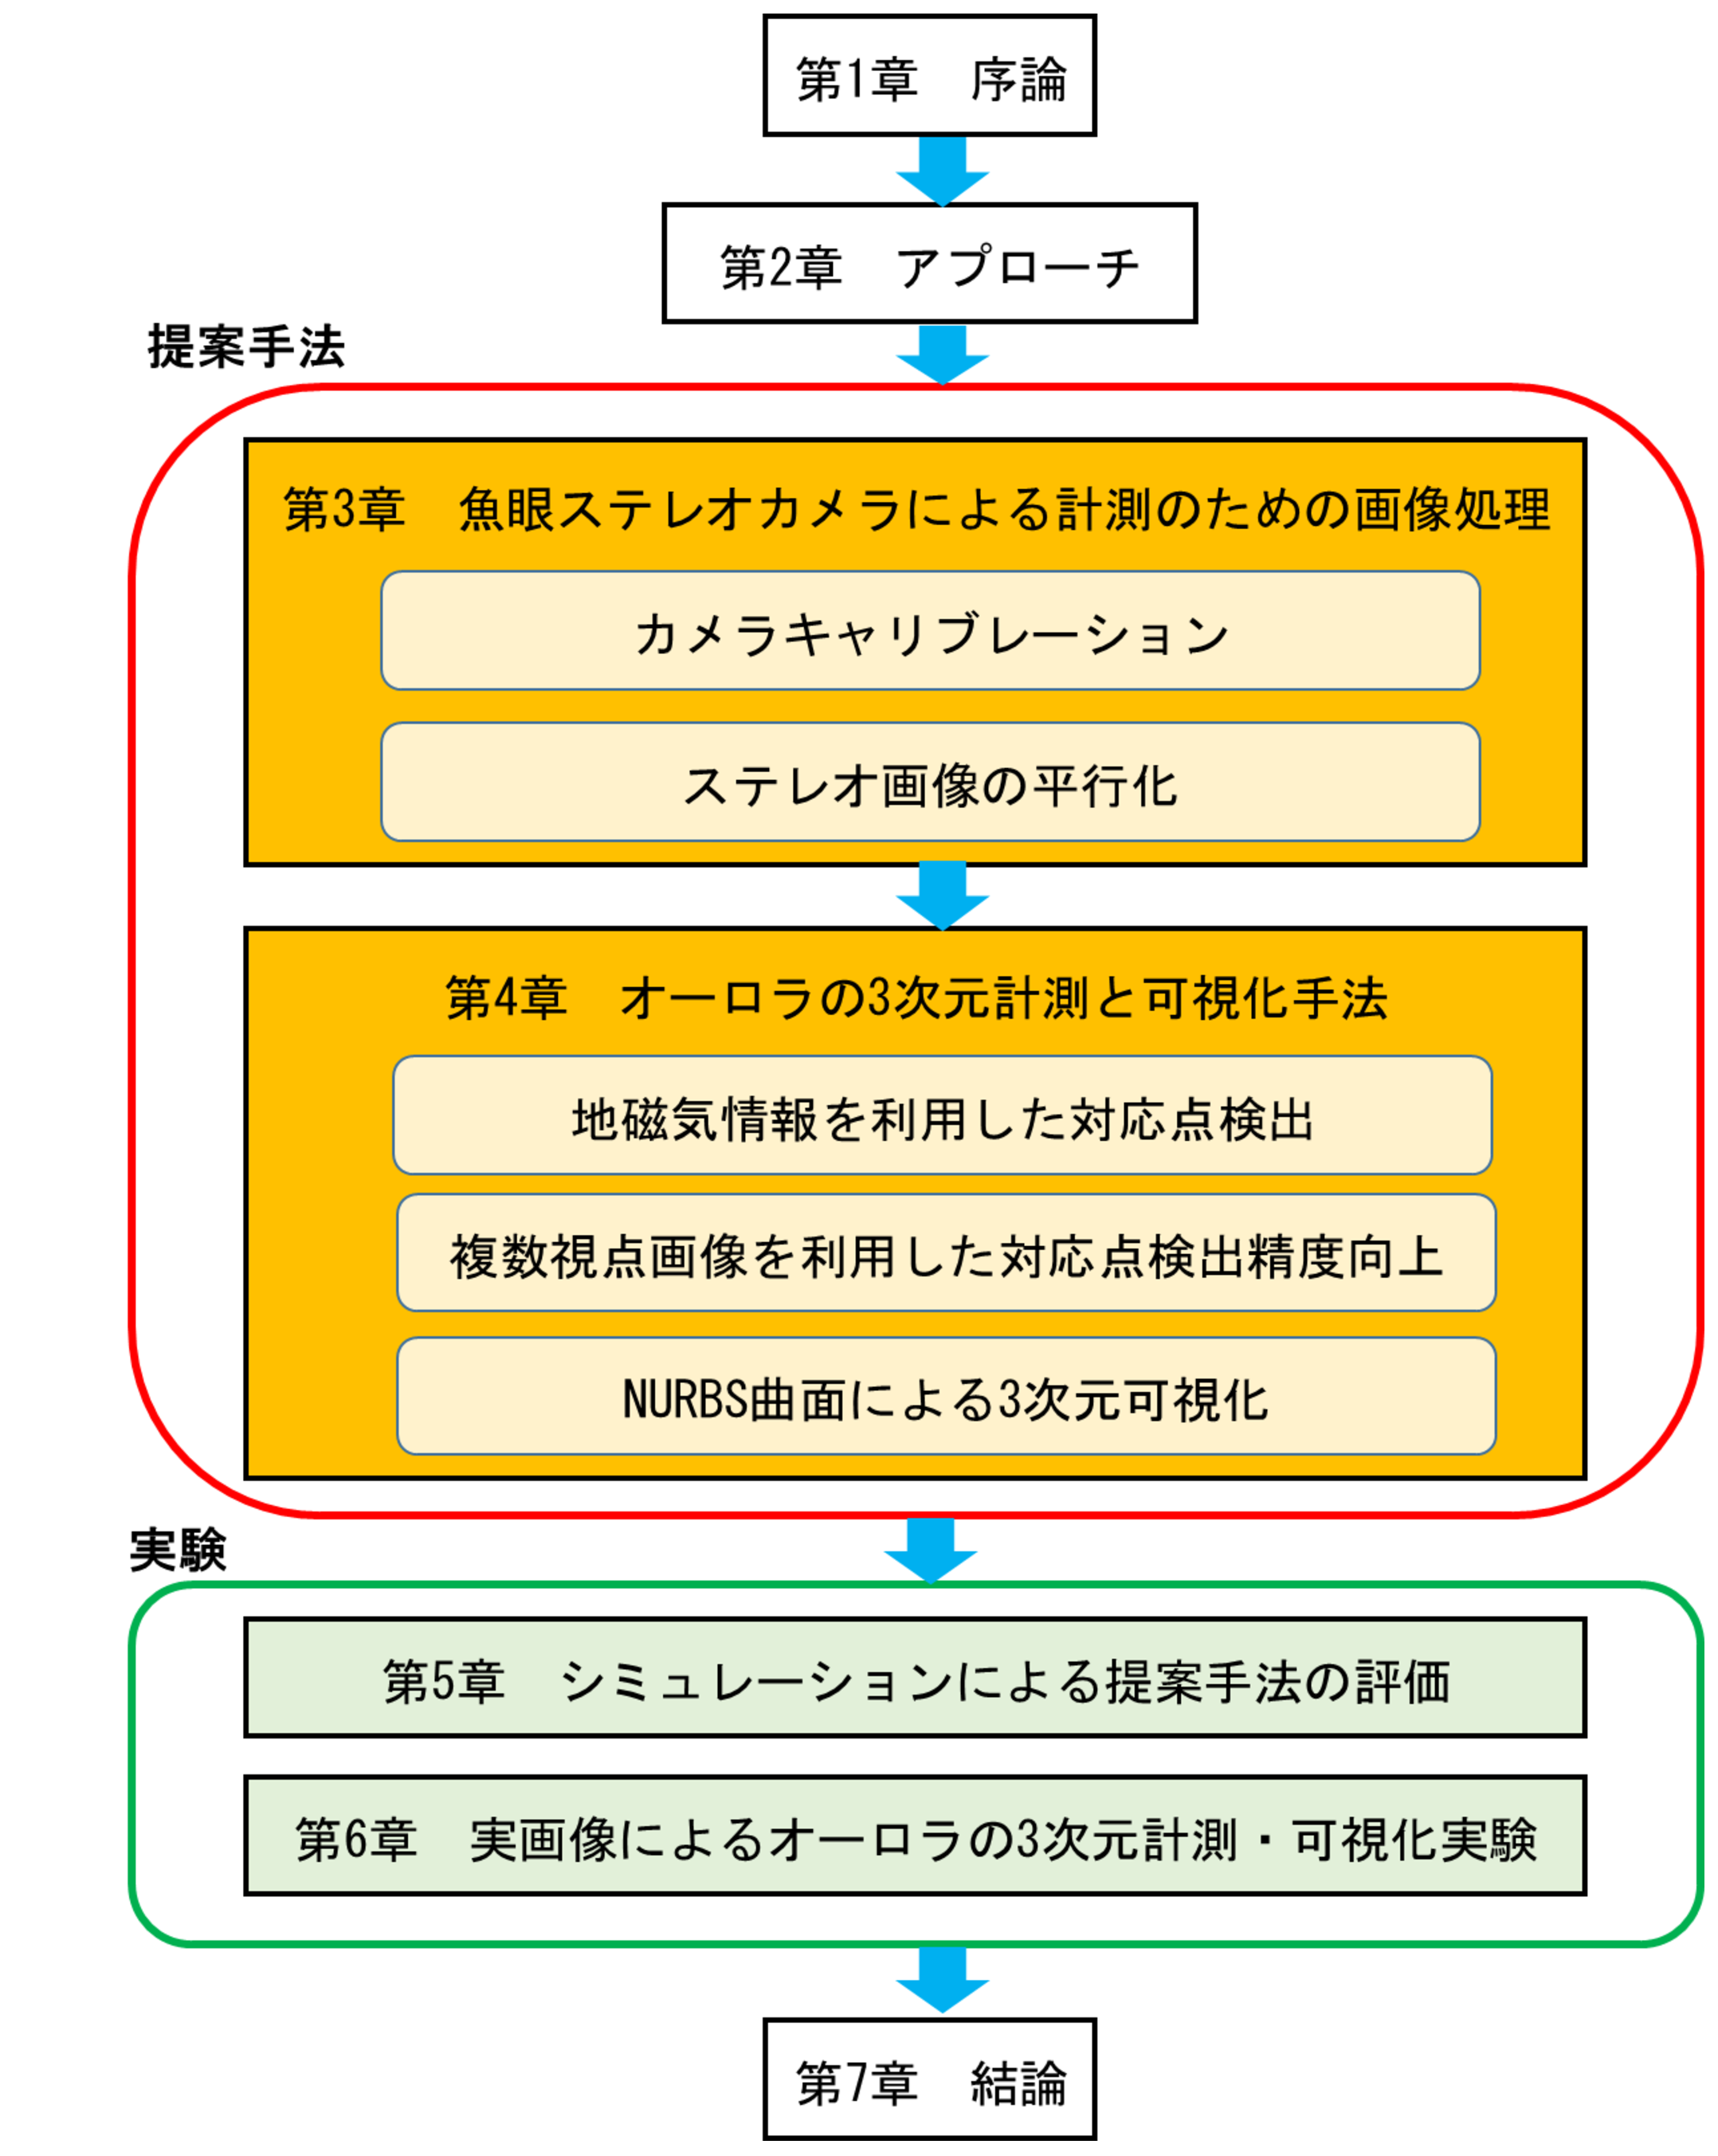
\includegraphics[width=11cm]{./chap1/eps/Thesis_flow.eps}
\caption{�{�_���̍\��}
\label{fig:Thesis_flow}
\end{center}
\end{figure}

\clearpage



%%%%%%%%%%%%%%%%%%%%%%%%%%%%%%%%%%%%%%%%%%%%%%%%%%%%%%%%%%%%%%%%%%%%%%%%%%%%%%%%%%%%%%%%%%%%%%%%%%%%%%%%%%%%%%%%%%%%%%%%%%%%%%%%%%%
%%% Local Variables:
%%% mode: katex
%%% TeX-master: "../thesis"
%%% End:

\chapter{本研究のアプローチ}
\label{chap:approach}
\minitoc

\thispagestyle{empty}

\newpage
%%%%%%%%%%%%%%%%%%%%%%%%%%%%%%%%%%%%%%%%%%%%%%%%%%%%%%%%%%%%%%%%%%%%%%%%%%%%%%%%%%%%%%%%%%%%%%%%%%%%%%%%%%%%%%%%%%%%%%%%%%%%%%%%%%%
\section{はじめに}
\label{sec:intro_chap2}

本章では,ヒトの運動のメカニズムを理解し,片麻痺患者の回復期のリハビリテーション(以下リハビリ)を日常的に支援する機器を開発するアプローチについて述べる.

%\ref{sec:problem_setteing_chap2}節にて,本研究における問題設定について述べる.

\ref{sec:approach_chap2}節にて,本手法のアプローチと解決すべき課題について述べる.
\ref{subsec:investigate_chap2}項にて,理学療法士のリハビリテーションにおける片麻痺患者への影響の調査について述べる.
\ref{subsec:analysys_chap2}項にて,理学療法士の技能を解析するアプローチについて述べる.
\ref{subsec:development_chap2}項にて,理学療法士の技能を応用する支援機器の開発のアプローチについて述べる.

\ref{sec:outro_chap2}節にて,本章のまとめを述べる.

\clearpage

%%%%%%%%%%%%%%%%%%%%%%%%%%%%%%%%%%%%%%%%%%%%%%%%%%%%%%%%%%%%%%%%%%%%%%%%%%%%%%%%%%%%%%%%%%%%%%%%%%%%%%%%%%%%%%%%%%%%%%%%%%%%%%%%%%%

%\section{問題設定}
%\label{sec:problem_setteing_chap2}
%第1章にて,が重要であることを述べた.\\
%
%また,\ref{sec:related_research_chap1}節にて,を述べた.などが例として挙げられる.\\
%
%また,同様に\ref{sec:related_research_chap1}節にて,であることを述べた.従って,本研究では利用する.\\
%
%上記を踏まえて,以下に本研究の問題設定をまとめる.
%\begin{itemize}
%\item 患者への影響を調査
%\item 技能を調査
%\item 支援機器を開発
%\end{itemize}
%
%このような問題設定の下,手法を提案する.
%
%
%\clearpage


%%%%%%%%%%%%%%%%%%%%%%%%%%%%%%%%%%%%%%%%%%%%%%%%%%%%%%%%%%%%%%%%%%%%%%%%%%%%%%%%%%%%%%%%%%%%%%%%%%%%%%%%%%%%%%%%%%%%%%%%%%%%%%%%%%%
\section{アプローチ}
\label{sec:approach_chap2}
\ref{sec:objective_chap1}節にて述べた通り,本研究の目的は理学療法士の介入による片麻痺患者への影響を調査,理学療法士の技能を解析,理学療法士の技能を活用した,起立動作の支援機器の開発の三つである.
それぞれの目的を達成するためのアプローチを次節で述べていく.\\

%\clearpage
%%%%%%%%%%%%%%%%%%%%%%%%%%%%%%%%%%%%%%%%%%%%%%%%%%%%%%%%%%%%%%%%%%%%%%%%%%%%%%%%%%%%%%%%%%%%%%%%%%%%%%%%%%%%%%%%%%%%%%%%%%%%%%%%%%%
\subsection{片麻痺患者への影響の調査}
\label{subsec:investigate_chap2}

理学療法士のリハビリテーションにより片麻痺患者にどのような影響があるのかを調査することを前述した.本項では,片麻痺患者への影響の調査方法について説明する.\\

起立動作は,年齢,関節角度,床反力,関節トルク,重心軌道,表面筋電図など多くの指標により調べられてきた.しかし,片麻痺患者に対してどの指標がより起立動作の特徴を捉えているか,有用な指標を抽出するような研究は行われていない\cite{長田2012}.

本研究では起立動作を運動学的な観点と表面筋電図から計算される筋シナジー構造から評価する.運動学的な観点の指標として,片麻痺患者の関節角度や重心(Center of Mass,以下CoM)の軌道を用いる.

起立動作のCoMについてはいくつかの報告がなされている.
\textcolor{red}{\cite{Mourey2000}と\cite{Yang2017}を引いて,高齢者や片麻痺患者は上体を深く曲げて起立することを記述}
%高齢者は筋肉量が低下しているため,起立の際には転倒の危険性が発生する.より安定した起立のために,若年者よりも上体を深く曲げることでCoMを足に近づけてから立ち上がる\cite{Mourey2000}.
%さらに,片麻痺患者になると健常な高齢者よりもCoMが足に近づいてから立ち上がることが分かっている\cite{Yang2017}.
\\

起立動作中の筋電図(Electromyogram,以下EMG)については以下のような報告がある.
\textcolor{red}{\cite{Silva2013}と\cite{Gross1998}を引いて,前脛骨筋の活動タイミングなどについて記述.}\\
%Silvaらは健常者と片麻痺患者を対象とし,ヒラメ筋と前脛骨筋のEMGを計測した\cite{Silva2013}.片麻痺患者において健常者よりも,麻痺と非麻痺の両側のヒラメ筋の活動タイミングが早く,麻痺側の前脛骨筋の活動タイミングが遅かったと報告している.
%また,Grossらは若年者と片麻痺患者を対象として前脛骨筋と大腿四頭筋のEMGを計測した\cite{Gross1998}.片麻痺患者において,健側の足の位置を変えることで前脛骨筋の大腿四頭筋の活動が増加することを報告した.

本研究ではヒトの運動のメカニズムを理解するべく,筋シナジー仮説を用いる.


\textcolor{red}{筋シナジー仮説とは何かを説明.}
\\

運動学的な指標や筋シナジー構造の詳細な算出方法や計測実験については第\ref{chap:investigation}章にて述べる.

%\clearpage
%%%%%%%%%%%%%%%%%%%%%%%%%%%%%%%%%%%%%%%%%%%%%%%%%%%%%%%%%%%%%%%%%%%%%%%%%%%%%%%%%%%%%%%%%%%%%%%%%%%%%%%%%%%%%%%%%%%%%%%%%%%%%%%%%%%
\subsection{理学療法士の技能解析}
\label{subsec:analysys_chap2}

片麻痺患者のリハビリテーション中において,理学療法士はどのような介入を行っているのかを調査することを前述した.本項では,理学療法士の技能の解析方法について説明する.\\

理学療法士の技能について,Tsusakaらは起立動作における理学療法士のスキル分析をしている\cite{Tsusaka2015}.
\textcolor{red}{スキル分析について記述.}\\

本研究では理学療法士の技能の調査方法として片麻痺患者に介入する腕の筋肉の表面筋電図を計測する.
理学療法士は図\ref{fig:view}に示すように,片麻痺患者の麻痺側の膝と骨盤後面に介入する.上肢の曲げ伸ばしをどのタイミングで行っているかを調査するため,理学療法士の腕の筋肉の表面筋電図を計測する.
\\

\begin{figure}[b]
	\begin{center}
		\includegraphics[width=8cm]{./Chap2/fig/view.eps}
		\caption{理学療法士による介入の様子}
		\label{fig:view}
	\end{center}
\end{figure}

理学療法士の技能の詳細な調査方法は第\ref{chap:analysys}章にて述べる.

%\clearpage

%%%%%%%%%%%%%%%%%%%%%%%%%%%%%%%%%%%%%%%%%%%%%%%%%%%%%%%%%%%%%%%%%%%%%%%%%%%%%%%%%%%%%%%%%%%%%%%%%%%%%%%%%%%%%%%%%%%%%%%%%%%%%%%%%%%
\subsection{起立動作の支援機器の開発}
\label{subsec:development_chap2}

本研究では理学療法士の技能を活用した,起立動作の支援機器の開発について前述した.
本項では,技能を活用した支援機器の従来研究について説明する.\\

\textcolor{red}{看護師の技能を活かした起立動作の支援システムを引く\cite{Chugo2007}.
	理学療法士のスキル活かした起立アシストロボットの開発を引く\cite{津坂2017}.
}\\



起立動作の支援機器の開発についての詳細な方法は第\ref{chap:development}章にて述べる.

\clearpage

%%%%%%%%%%%%%%%%%%%%%%%%%%%%%%%%%%%%%%%%%%%%%%%%%%%%%%%%%%%%%%%%%%%%%%%%%%%%%%%%%%%%%%%%%%%%%%%%%%%%%%%%%%%%%%%%%%%%%%%%%%%%%%%%%%%
\section{おわりに}
\label{sec:outro_chap2}

本章では,本研究のアプローチについて述べた.

%まず\ref{sec:problem_setteing_chap2}節にて,本研究において解決するべき課題について述べた.

\ref{sec:approach_chap2}節にて,本手法のアプローチと解決すべき課題について述べた.
\ref{subsec:investigate_chap2}節にて,理学療法士によるリハビリ中の片麻痺患者の起立動作の変化を調査するアプローチについて述べた.
\ref{subsec:analysys_chap2}項にて,理学療法士の技能を解析するためのアプローチについて述べた.
\ref{subsec:development_chap2}項にて,支援機器を開発するアプローチについて述べた.\\

次章では,技能解析について詳しく説明する.

\clearpage

%%%%%%%%%%%%%%%%%%%%%%%%%%%%%%%%%%%%%%%%%%%%%%%%%%%%%%%%%%%%%%%%%%%%%%%%%%%%%%%%%%%%%%%%%%%%%%%%%%%%%%%%%%%%%%%%%%%%%%%%%%%%%%%%%%%
%%% Local Variables:
%%% mode: katex
%%% TeX-master: "../thesis"
%%% End:

\chapter{リハビリテーションによる片麻痺患者への影響の調査}
\label{chap:investigation}
\minitoc

\thispagestyle{empty}

\newpage
%%%%%%%%%%%%%%%%%%%%%%%%%%%%%%%%%%%%%%%%%%%%%%%%%%%%%%%%%%%%%%%%%%%%%%%%%%%%%%%%%%%%%%%%%%%%%%%%%%%%%%%%%%%%%%%%%%%%%%%%%%%%%%%%%%%
\section{はじめに}
\label{sec:intro_chap3}

本章では,理学療法士のリハビリテーションによる片麻痺患者への影響について述べる.

\ref{sec:method_chap3}節にて,片麻痺患者への影響の調査方法の概要について述べる.本研究では片麻痺患者の重心軌道,関節角度といった運動学的な手法や筋シナジー構造による評価を評価手法として採用する.\ref{subsec:method_kinematics_chap3}項にて,重心軌道や関節角度の算出方法について述べる.\ref{subsec:method_synergy_chap3}項にて,筋シナジー構造について述べる.

\ref{sec:experiment_chap3}節にて,片麻痺患者に対して行った計測実験について述べる.\ref{subsec:subject_chap3}項にて,対象とした片麻痺患者の属性について述べる.\ref{subsec:device_chap3}項にて,計測に用いた装置について述べる.\ref{subsec:method_chap3}項にて,計測実験の手順について述べる.

\ref{sec:result_chap3}節にて,計測実験の結果について述べる.\ref{subsec:result_kinematics_chap3}項にて,重心軌道や関節角度の調査結果について述べる.\ref{subsec:result_synergy_chap3}項にて,筋シナジー構造の調査結果について述べる.

\ref{sec:discussion_chap3}節にて,計測実験の結果の考察について述べる.\ref{subsec:discussion_kinematics_chap3}項にて,重心軌道や関節角度の調査結果の考察について述べる.\ref{subsec:discussion_synergy_chap3}項にて,筋シナジー構造の調査結果の考察について述べる.

\ref{sec:outro_chap3}節にて,本章のまとめを述べる.

\textcolor{red}{改ページする予定です.}
%\clearpage

%%%%%%%%%%%%%%%%%%%%%%%%%%%%%%%%%%%%%%%%%%%%%%%%%%%%%%%%%%%%%%%%%%%%%%%%%%%%%%%%%%%%%%%%%%%%%%%%%%%%%%%%%%%%%%%%%%%%%%%%%%%%%%%%%%%
%%%%%%%%%%%%%%%%%%%%%%%%%%%%%%%%%%%%%%%%%%%%%%%%%%%%%%%%%%%%%%%%%%%%%%%%%%%%%%%%%%%%%%%%%%%%%%%%%%%%%%%%%%%%%%%%%%%%%%%%%%%%%%%%%%%
\section{片麻痺患者への影響の調査方法}
\label{sec:method_chap3}
\ref{subsec:investigate_chap2}項にて,であることを述べた.本節では,理学療法士のリハビリテーションによる片麻痺患者への影響の調査方法の概要について述べる.\\

片麻痺患者のリハビリにおける起立動作の調査方法の概要を図\ref{fig:approach_hemi}に示す.本研究ではモーションキャプチャシステム,無線筋電計,床反力計を用いて片麻痺患者の運動を計測する.

モーションキャプチャシステムでは患者に貼り付けたモーションキャプチャ用のマーカの位置を計測し,関節角度や重心(Center of Mass,以下CoM)軌道が算出可能である.
算出方法は\ref{subsec:method_kinematics_chap3}項にて,述べる.

無線筋電計では患者に貼り付ることで表面筋電図(Electromyogram,以下EMG)が計測可能である.
無線筋電計を用いて筋シナジー構造を算出する方法を\ref{subsec:method_synergy_chap3}項にて述べる.\\

%\begin{figure}[b]
%	\begin{center}
%		\includegraphics[width=8cm]{./Chap3/fig/approach_hemi.eps}
%		\caption{片麻痺患者の起立動作の調査方法の概要}
%		\label{fig:approach_hemi}
%	\end{center}
%\end{figure}

\subsection{運動学的による解析方法}
\label{subsec:method_kinematics_chap3}
本研究では運動学的な解析手法として重心軌道や関節角度を算出する方法を採用する.\textcolor{red}{計算方法を述べる.}\\

\subsection{筋シナジー構造による解析方法}
\label{subsec:method_synergy_chap3}
本研究では筋シナジー構造を解析することで,リハビリテーションによる片麻痺患者への影響を調査する.\textcolor{red}{計算方法を述べる.}\\

\textcolor{red}{改ページする予定です.}
%\clearpage
%%%%%%%%%%%%%%%%%%%%%%%%%%%%%%%%%%%%%%%%%%%%%%%%%%%%%%%%%%%%%%%%%%%%%%%%%%%%%%%%%%%%%%%%%%%%%%%%%%%%%%%%%%%%%%%%%%%%%%%%%%%%%%%%%%%
%%%%%%%%%%%%%%%%%%%%%%%%%%%%%%%%%%%%%%%%%%%%%%%%%%%%%%%%%%%%%%%%%%%%%%%%%%%%%%%%%%%%%%%%%%%%%%%%%%%%%%%%%%%%%%%%%%%%%%%%%%%%%%%%%%%
\section{片麻痺患者の計測実験}
\label{sec:experiment_chap3}
本章では片麻痺患者へ行った実験について述べる.下記に述べる実験は森之宮病院倫理委員会の承認を受け,実施された.

%%%%%%%%%%%%%%%%%%%%%
\subsection{被験者}
\label{subsec:subject_chap3}
対象とした片麻痺患者の属性について述べる.

%%%%%%%%%%%%%%%%%%%%%
\subsection{計測装置}
\label{subsec:device_chap3}
計測に用いた装置について述べる.

%%%%%%%%%%%%%%%%%%%%%
\subsection{実験手順}
\label{subsec:method_chap3}
計測実験の手順について述べる.

\textcolor{red}{改ページする予定です.}
%\clearpage
%%%%%%%%%%%%%%%%%%%%%%%%%%%%%%%%%%%%%%%%%%%%%%%%%%%%%%%%%%%%%%%%%%%%%%%%%%%%%%%%%%%%%%%%%%%%%%%%%%%%%%%%%%%%%%%%%%%%%%%%%%%%%%%%%%%
%%%%%%%%%%%%%%%%%%%%%%%%%%%%%%%%%%%%%%%%%%%%%%%%%%%%%%%%%%%%%%%%%%%%%%%%%%%%%%%%%%%%%%%%%%%%%%%%%%%%%%%%%%%%%%%%%%%%%%%%%%%%%%%%%%%
\section{実験結果}
\label{sec:result_chap3}

%%%%%%%%%%%%%%%%%%%%%
\subsection{運動学的な調査の結果}
\label{subsec:result_kinematics_chap3}
重心軌道や関節角度の調査結果について述べる.

%%%%%%%%%%%%%%%%%%%%%
\subsection{筋シナジー構造の調査の結果}
\label{subsec:result_synergy_chap3}
筋シナジー構造の調査結果について述べる.

\textcolor{red}{改ページする予定です.}
%\clearpage
%%%%%%%%%%%%%%%%%%%%%%%%%%%%%%%%%%%%%%%%%%%%%%%%%%%%%%%%%%%%%%%%%%%%%%%%%%%%%%%%%%%%%%%%%%%%%%%%%%%%%%%%%%%%%%%%%%%%%%%%%%%%%%%%%%%
%%%%%%%%%%%%%%%%%%%%%%%%%%%%%%%%%%%%%%%%%%%%%%%%%%%%%%%%%%%%%%%%%%%%%%%%%%%%%%%%%%%%%%%%%%%%%%%%%%%%%%%%%%%%%%%%%%%%%%%%%%%%%%%%%%%
\section{考察}
\label{sec:discussion_chap3}

%%%%%%%%%%%%%%%%%%%%%
\subsection{運動学的な調査の結果}
\label{subsec:discussion_kinematics_chap3}
重心軌道や関節角度の考察について述べる.

%%%%%%%%%%%%%%%%%%%%%
\subsection{筋シナジー構造の考察}
\label{subsec:discussion_synergy_chap3}
筋シナジー構造の考察について述べる.

\textcolor{red}{改ページする予定です.}
%\clearpage
%%%%%%%%%%%%%%%%%%%%%%%%%%%%%%%%%%%%%%%%%%%%%%%%%%%%%%%%%%%%%%%%%%%%%%%%%%%%%%%%%%%%%%%%%%%%%%%%%%%%%%%%%%%%%%%%%%%%%%%%%%%%%%%%%%%
\section{おわりに}
\label{sec:outro_chap3}
本章では,片麻痺患者へ行った実験について述べた.

\ref{sec:method_chap3}節にて,片麻痺患者への影響の調査方法の概要について述べた.本研究では片麻痺患者の重心軌道,関節角度といった運動学的な手法や筋シナジー構造による評価を評価手法として採用した.\ref{subsec:method_kinematics_chap3}項にて,重心軌道や関節角度の算出方法について述べた.\ref{subsec:method_synergy_chap3}項にて,筋シナジー構造について述べた.

\ref{sec:experiment_chap3}節にて,片麻痺患者に対して行った計測実験について述べた.\ref{subsec:subject_chap3}項にて,対象とした片麻痺患者の属性について述べた.\ref{subsec:device_chap3}項にて,計測に用いた装置について述べた.\ref{subsec:method_chap3}項にて,計測実験の手順について述べた.

\ref{sec:result_chap3}節にて,計測実験の結果について述べた.\ref{subsec:result_kinematics_chap3}項にて,重心軌道や関節角度の調査結果について述べた.\ref{subsec:result_synergy_chap3}項にて,筋シナジー構造の調査結果について述べた.

\ref{sec:discussion_chap3}節にて,計測実験の結果の考察について述べた.\ref{subsec:discussion_kinematics_chap3}項にて,重心軌道や関節角度の調査結果の考察について述べた.\ref{subsec:discussion_synergy_chap3}項にて,筋シナジー構造の調査結果の考察について述べた.\\

次章では,理学療法士の技能の解析について説明する.

\clearpage

%%%%%%%%%%%%%%%%%%%%%%%%%%%%%%%%%%%%%%%%%%%%%%%%%%%%%%%%%%%%%%%%%%%%%%%%%%%%%%%%%%%%%%%%%%%%%%%%%%%%%%%%%%%%%%%%%%%%%%%%%%%%%%%%%%%
%%% Local Variables:
%%% mode: katex
%%% TeX-master: "../thesis"
%%% End:

\chapter{位置推定}
\thispagestyle{empty}
\label{chap4}
\minitoc

\newpage
%%%%%%%%%%%%%%%%%%%%%%%%%%%%%%%%%%%%%%%%%%%%%%%%%%%%%%%%%%%%%%%%%%%%%%%%%%%%%%%
%==============================================================================
% 4.1
%==============================================================================
\section{はじめに}

本章では,位置$\bm{P}$を推定する手法について述べる.

4.2節にて,手法の概要について述べる.

4.3節にて,特徴量の計算について述べる.

4.4節にて,$xy$座標の推定方法について述べる.

4.5節にて,$z$座標の推定方法について述べる.


\clearpage
%==============================================================================
% 4.2
%==============================================================================
\section{位置推定の概要}

位置推定では,各エッジ点とそれに対応する単位球面勾配ベクトル,姿勢$\bm{O}$,ラインマップからカメラの位置$\bm{P}$を推定する.
図\ref{fig:derotation}に示すように,ワールド座標系から姿勢$\bm{O}$の分ずれているカメラ座標系$x_{\rm{sph}}y_{\rm{sph}}z_{\rm{sph}}$を$\bm{O}^{-1}$回転させることでワールド座標系と向きが一致した状態に変換して位置を推定する.変換後のカメラ座標系を$x'_{\rm{sph}}y'_{\rm{sph}}z'_{\rm{sph}}$とする.
\\

\begin{figure}[b]
 \begin{center}
 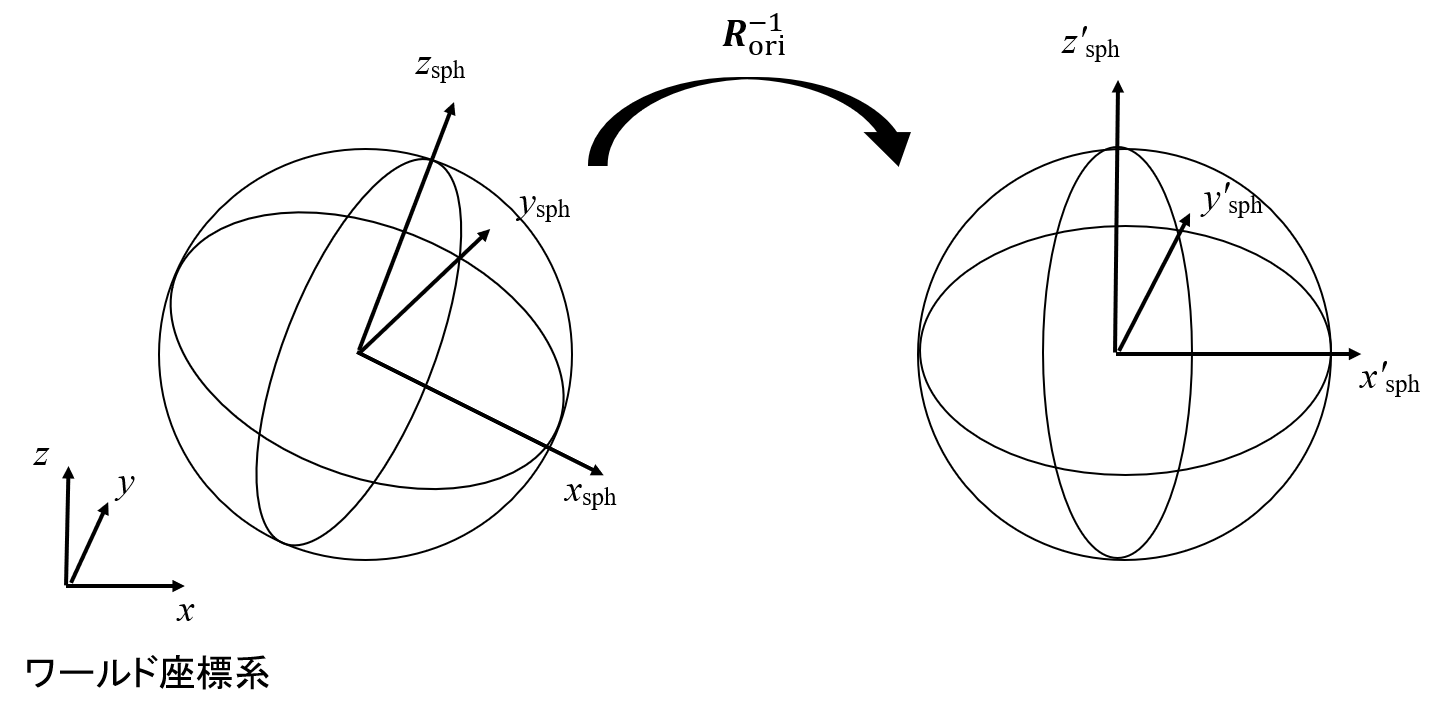
\includegraphics[width=0.85\columnwidth]{./chap4/fig/derotation.png}
 \caption{ワールド座標系の向きと一致させるようなカメラ座標系の回転}
 \label{fig:derotation}
 \end{center}
\end{figure}

位置推定では,ワールド座標系における各軸方向の直線が球面に投影されたとき,それぞれの軸方向を法線ベクトルとする大円と交わる点の分布を特徴量とする.
この特徴量は,$y'_{\rm{sph}}z'_{\rm{sph}}$平面,$x'_{\rm{sph}}z'_{\rm{sph}}$平面,$x'_{\rm{sph}}y'_{\rm{sph}}$平面のそれぞれにおける単位円上の点の集合で表される.
例えば,図\ref{fig:feature_x}に示すように,青い実線で示す$x$軸方向に伸びる直線は青い破線で示す線のように球面に投影され,この破線と$x'_{\rm{sph}}$方向を法線ベクトルとする大円の交点は$y'_{\rm{sph}}z'_{\rm{sph}}$平面における単位円上に存在する.
すべての$x$軸方向の直線について同様に交点を計算すると,$y'_{\rm{sph}}z'_{\rm{sph}}$平面における単位円上の点の集合が得られる.
これと同様に,$y$軸方向に伸びる直線から$x'_{\rm{sph}}z'_{\rm{sph}}$平面における単位円上の点の集合が得られ(図\ref{fig:feature_y}),$z$軸方向に伸びる直線から$x'_{\rm{sph}}y'_{\rm{sph}}$平面における単位円上の点の集合が得られる(図\ref{fig:feature_z}).
これらをそれぞれ,$yz$特徴量,$xz$特徴量,$xy$特徴量と呼ぶ.
これらの特徴量は各カメラ位置において一意に定まるため,推定する画像の特徴量とラインマップから計算する各位置における特徴量を比較し,最も類似度の高い位置を探索することによりカメラの位置を推定することができる.
\\

\begin{figure}[tb]
 \begin{center}
 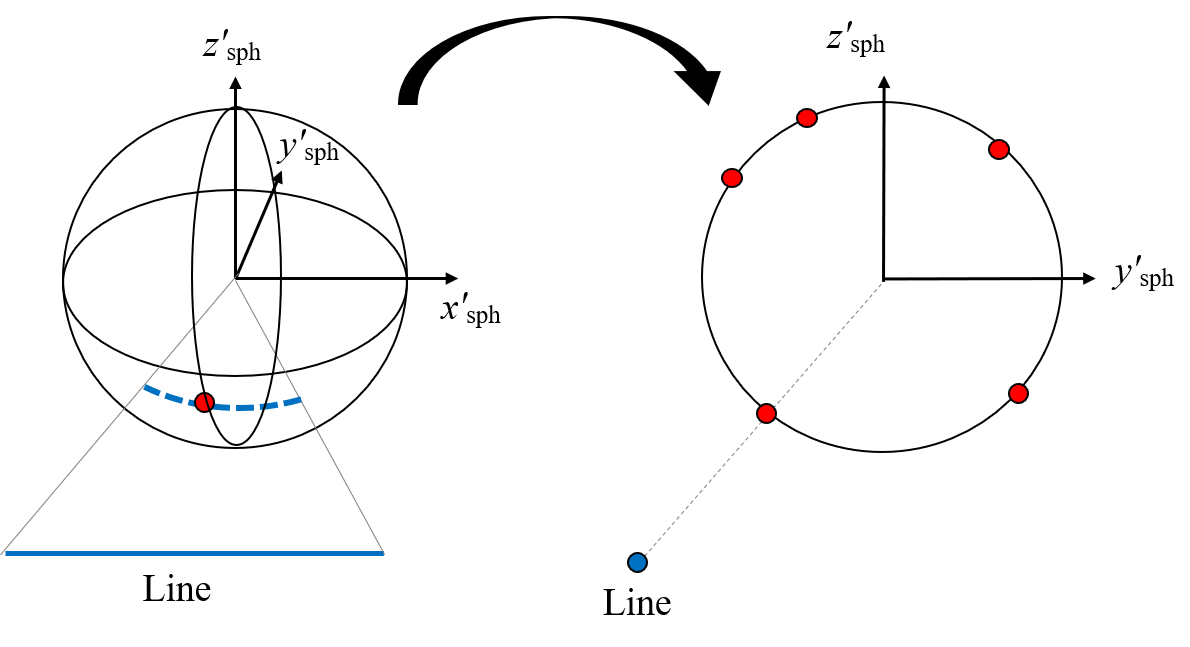
\includegraphics[width=0.85\columnwidth]{./chap4/fig/feature_x.png}
 \caption{$x$軸方向の直線から得られる$y'_{\rm{sph}}z'_{\rm{sph}}$平面における単位円上の点の集合}
 \label{fig:feature_x}
 \end{center}
\end{figure}

\begin{figure}[tb]
 \begin{center}
 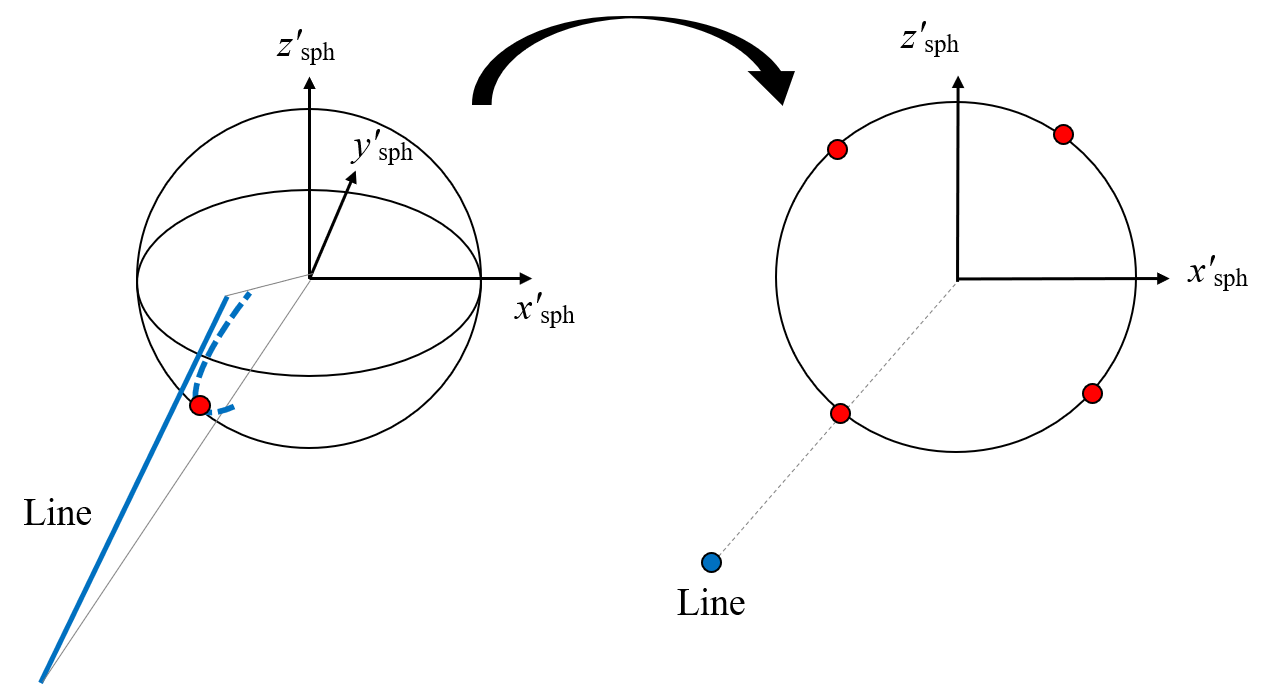
\includegraphics[width=0.85\columnwidth]{./chap4/fig/feature_y.png}
 \caption{$y$軸方向の直線から得られる$x'_{\rm{sph}}z'_{\rm{sph}}$平面における単位円上の点の集合}
 \label{fig:feature_y}
 \end{center}
\end{figure}

\clearpage

\begin{figure}[tb]
 \begin{center}
 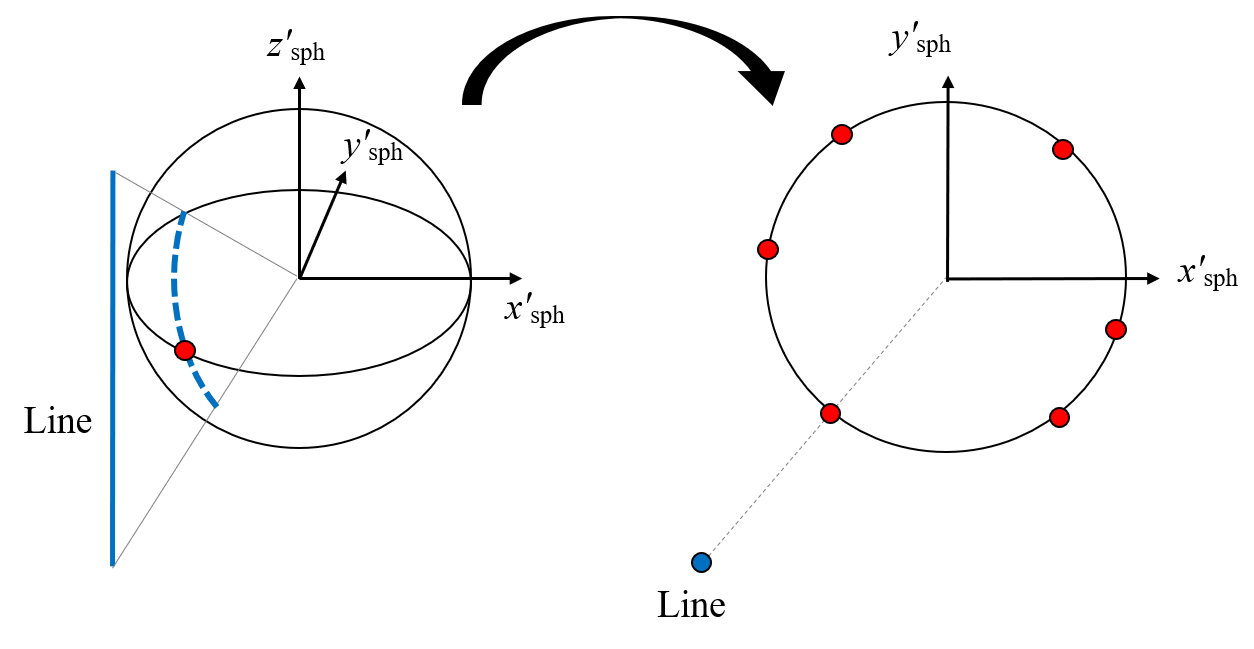
\includegraphics[width=0.85\columnwidth]{./chap4/fig/feature_z.png}
 \caption{$z$軸方向の直線から得られる$x'_{\rm{sph}}y'_{\rm{sph}}$平面における単位円上の点の集合}
 \label{fig:feature_z}
 \end{center}
\end{figure}


ここで,各軸方向の直線から得られる特徴量は,その軸方向のカメラ移動に依存せずに定まる.
つまり,$x$軸方向の直線から得られる$yz$特徴量はカメラの$yz$座標にのみにより定まり,$y$軸方向の直線から得られる$xz$特徴量はカメラの$xz$座標にのみにより定まり,$z$軸方向の直線から得られる$xy$特徴量はカメラの$xy$座標にのみにより定まる.
これを利用して,はじめに1つの特徴量を用いて2自由度の推定を行い,次に残りの特徴量から1つを選んで残りの1自由度の推定を行うことで,2自由度の推定と1自由度の推定に分離して行う.
本研究では,はじめに$xy$特徴量を用いた2次元の探索により$xy$座標を推定し,その後$xz$特徴量と推定された$x$座標を用いた1次元の探索により$z$座標を推定した.
\\

位置推定の流れを図\ref{fig:flow4}に示す.
まず,各エッジ点とそれに対応する単位球面勾配ベクトル,姿勢$\bm{O}$から推定する画像の特徴量を計算し,$xy$特徴量と$xz$特徴量を得る.
次に,得られた$xy$特徴量とラインマップから$xy$座標の推定を行い,推定値$x^*,\ y^*$を求める.
最後に,$xz$特徴量,推定値$x^*$,ラインマップから$z$座標の推定を行い,推定値$z^*$を求める.
以上の流れで,カメラの位置$\bm{P}$の推定値$\bm{P}^*=[x^*,\ y^*,\ z^*]^{\mathrm{T}}$を得る.


\begin{figure}[tb]
 \begin{center}
 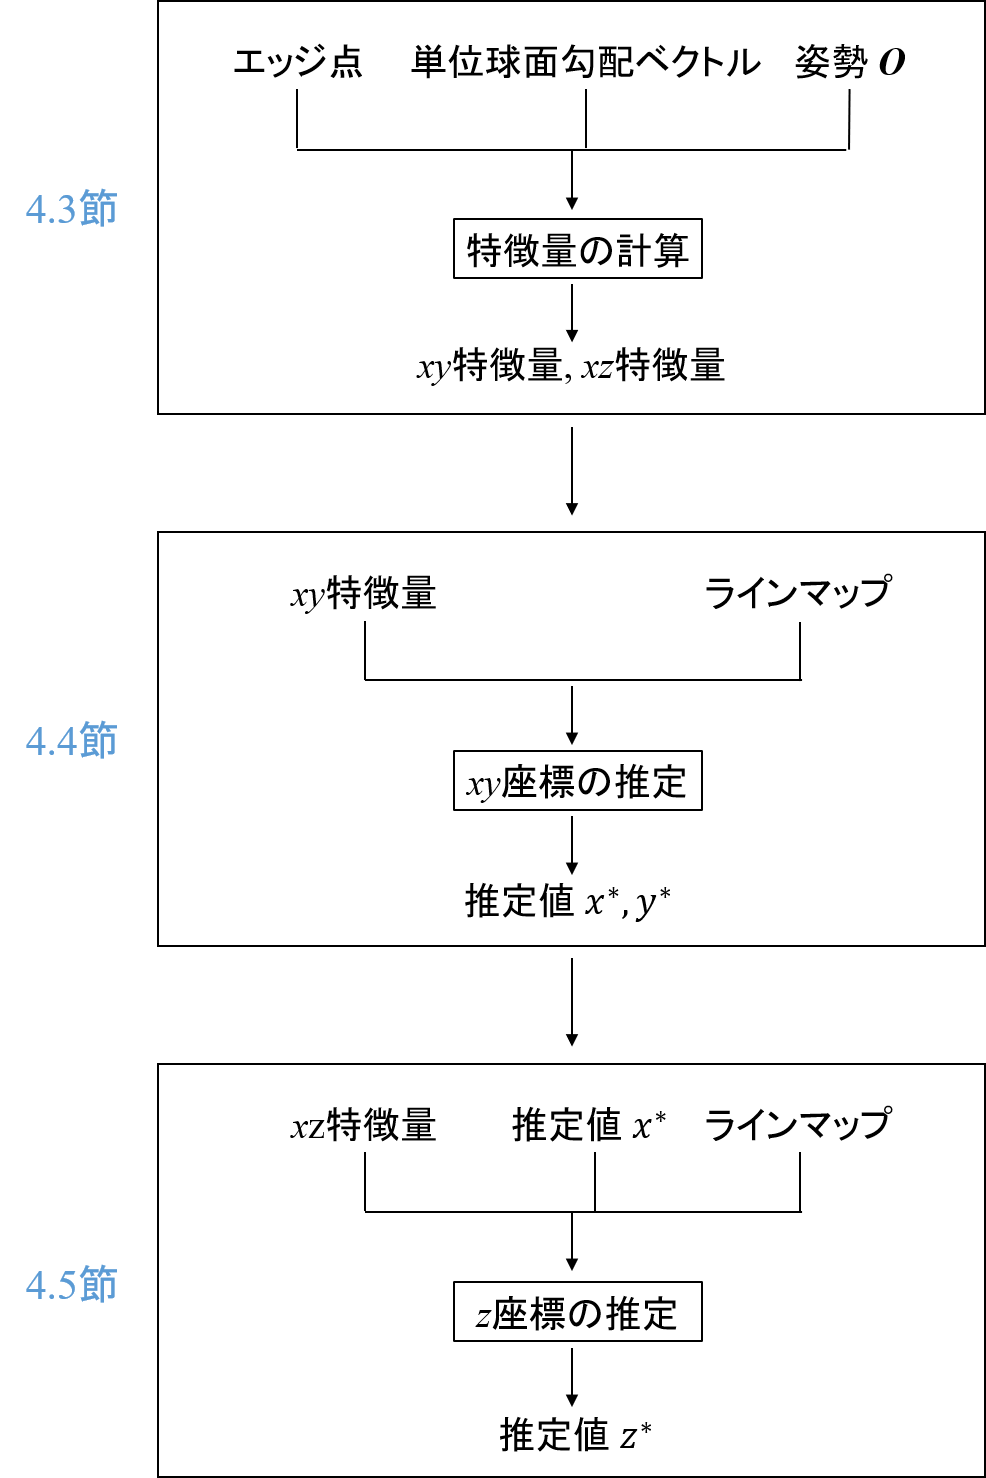
\includegraphics[width=0.7\columnwidth]{./chap4/fig/flow4.png}
 \vspace{5mm}
 \caption{位置推定の流れ}
 \label{fig:flow4}
 \end{center}
\end{figure}

\clearpage
%==============================================================================
% 4.3
%==============================================================================
\section{特徴量の計算}

\subsection{エッジ点の分類}

エッジ点とそれに対応する単位球面勾配ベクトルの組から$xy$特徴及び$xz$特徴量を得るためには,それぞれの勾配ベクトルがどの軸方向の直線によるエッジ点から得られたものかによって分類する必要がある.
姿勢を推定したあと,3平面のうち最も近い平面からの距離が閾値以上の単位勾配ベクトルをoutlierとして除去する.
残った単位球面勾配ベクトルをそれぞれ最も近い平面ごとに分類することで,元の入力画像におけるエッジ点を,どの方向の直線に属するものかで3つのグループに分類する.
分類されたエッジ点の例を図\ref{fig:classified}に示す.
赤色のエッジ点が$x$軸方向の直線によるエッジ点,緑色のエッジ点が$y$軸方向の直線によるエッジ点,青色のエッジ点が$z$軸方向の直線によるエッジ点をそれぞれ表している.
\\

\begin{figure}[b]
 \begin{center}
 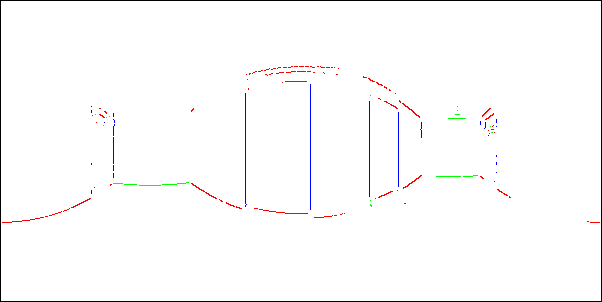
\includegraphics[width=0.7\columnwidth]{./chap4/fig/edge_inlier.png}
 \caption{分類されたエッジ点}
 \label{fig:classified}
 \end{center}
\end{figure}

\clearpage

\subsection{$xy$特徴量}

$xy$座標の推定に用いる$xy$特徴量には,$z$軸方向の直線が球上に投影される直線と全天球カメラの$x_{sph}y_{sph}$平面の交点の分布$(x_k,y_k)\ (k=1, 2,..., n)$を用いる.
特徴量の計算では,4.3.1項で分類したエッジ点のうち,$z$軸方向の直線に属するものを抽出して行う.
図\ref{fig:classified}に青色で示されたエッジ点がこれに該当する.
図\ref{fig:feature_xy}に示すように,抽出されたエッジ点座標を$(u_k, v_k)\ (k=1, 2,..., n)$,画像の幅を$w$とすると,交点$(x_k,y_k)$は以下の式によって求められる.

\begin{equation}
   \left(x_k,\ y_k\right) = \left(-\sin\frac{2\pi u_k}{w},\ -\cos\frac{2\pi u_k}{w}\right).
\end{equation}

\begin{figure}[b]
 \begin{center}
 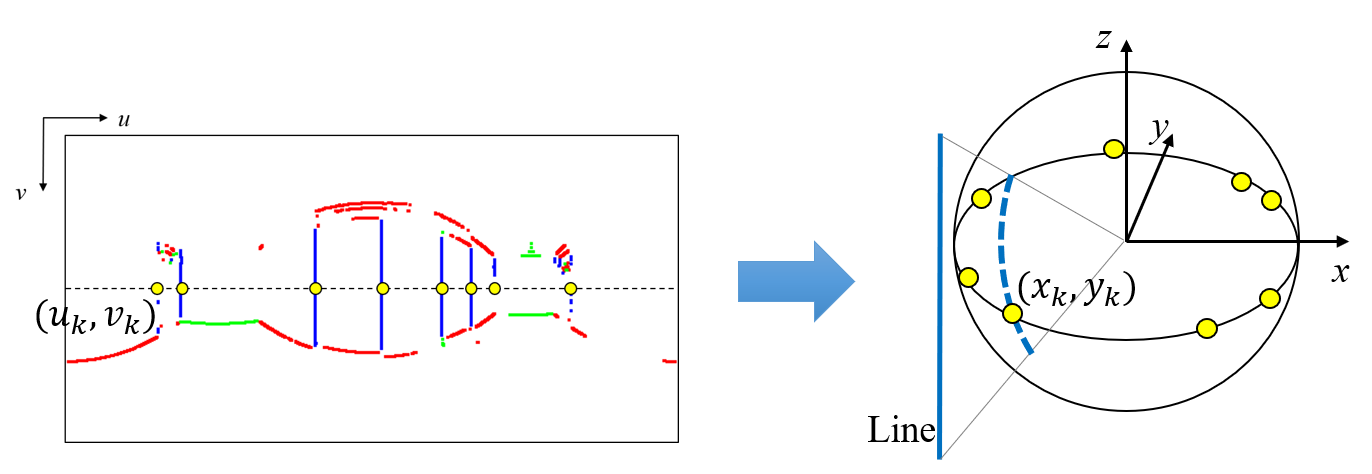
\includegraphics[width=1.0\columnwidth]{./chap4/fig/feature_xy.png}
 \vspace{5mm}
 \caption{$xy$特徴量($x_{sph}y_{sph}$平面)の計算}
 \label{fig:feature_xy}
 \end{center}
\end{figure}

\clearpage
\subsection{$xz$特徴量}
$z$座標の推定に用いる$xz$特徴量には,$y$軸方向の直線が球上に投影される直線と全天球カメラの$x_{sph}z_{sph}$平面の交点の分布$(x_k,z_k)\ (k=1, 2,..., n)$を用いる.
まず,図\ref{fig:classified}に示すエッジ画像を$x$軸回りに-90 deg回転させることで,図\ref{fig:rotated_edge}のようなエッジ画像に変換する.
特徴量の計算では,このエッジ画像内のエッジ点のうち,$y$軸方向の直線に属するものを抽出して行う.
図\ref{fig:rotated_edge}に緑色で示されたエッジ点がこれに該当する.
図\ref{fig:feature_xz}に示すように,抽出されたエッジ点座標を$(u_k, v_k)\ (k=1, 2,..., n)$,画像の幅を$w$ pixelとすると,交点$(x_k,z_k)$は以下の式によって求められる.

\begin{equation}
   \left(x_k,\ z_k\right) = \left(-\sin\frac{2\pi u_k}{w},\ -\cos\frac{2\pi u_k}{w}\right).
\end{equation}

\begin{figure}[b]
 \begin{center}
 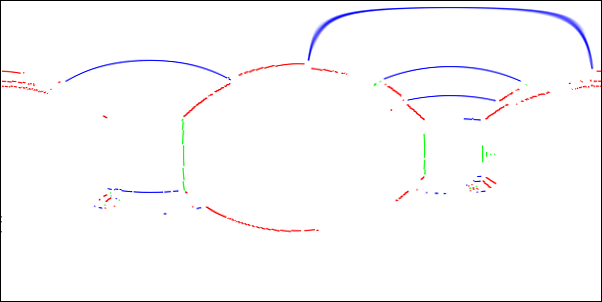
\includegraphics[width=0.7\columnwidth]{./chap4/fig/rotated_edge.png}
 \vspace{5mm}
 \caption{$x$軸回りに-90 deg回転させたエッジ画像}
 \label{fig:rotated_edge}
 \end{center}
\end{figure}


\begin{figure}[b]
 \begin{center}
 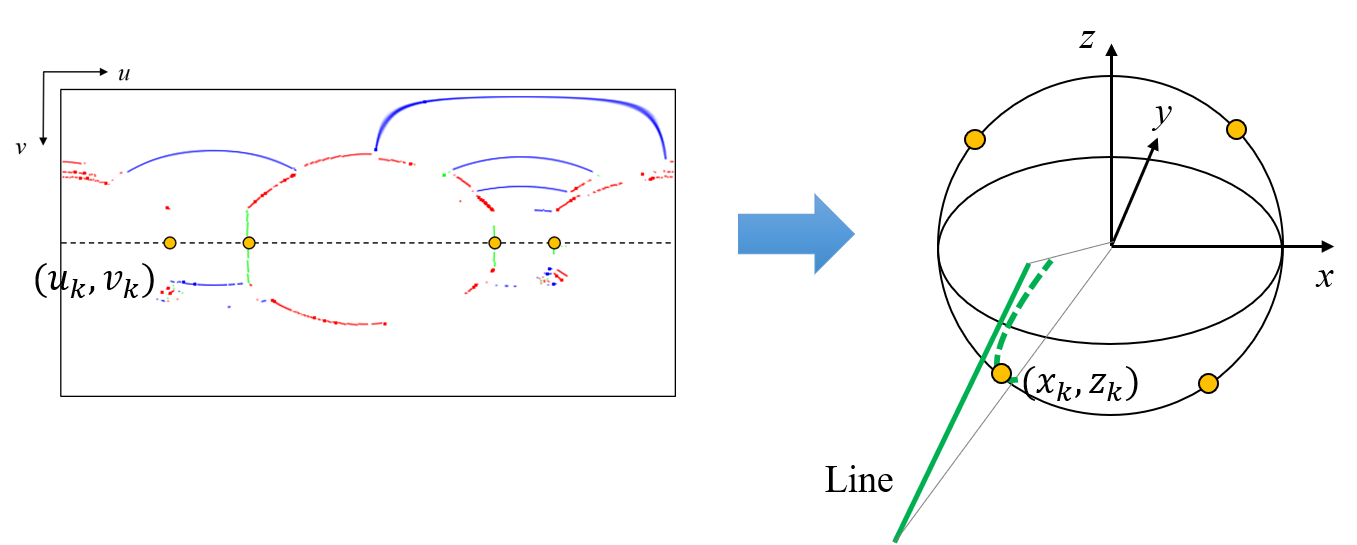
\includegraphics[width=1.0\columnwidth]{./chap4/fig/feature_xz.png}
 \vspace{5mm}
 \caption{$xz$特徴量($x_{sph}z_{sph}$平面)の計算}
 \label{fig:feature_xz}
 \end{center}
\end{figure}


\clearpage
%==============================================================================
% 4.4
%==============================================================================
\section{$xy$座標の推定}

$xy$座標の推定では,$z$座標を固定し,2次元の最適化によって推定する.
図\ref{fig:search_xy}に座標$(x,y)$における全天球カメラを上から見た図を示す.
緑色の点が上記の方法で求めた交点,赤色の点がラインマップから求めた,座標$(x,y)$から遮蔽されることなく見えるz軸方向の直線をそれぞれ表している.
画像から全ての直線を検出できるとは限らないため交点と直線の数は必ずしも一致せず,交点の数を$n$,直線の数を$m$とする.
各交点と直線の距離を,全天球カメラ座標系においてそれぞれが成す角によって定義し,すべての交点に対する最も近い直線までの距離の二乗和が最小となるような座標$(x,y)$を推定値とする.
交点の座標を$(x_k,y_k)\ (k=1, 2,..., n)$,ラインマップにおける$z$軸方向の直線の$xy$座標を$(x_l, y_l)\ (l=1, 2,...,m)$とすると,これらの距離$d_{k,l}$は,以下の式で得られる.
\begin{equation}
   d_{k,l} = \cos^{-1}\left(\frac{x_k(x_l-x)+y_k(y_l-y)}{\sqrt{(x_l-x)^2+(y_l-y)^2}}\right).
\end{equation}

$d_{k,l}\ (l=1,2,...,m)$のうち,最も小さいものを$d_k$とする.

\begin{equation}
   d_k = \min\left(d_{k,1},\ d_{k,2},\cdots,\ d_{k,m}\right).
\end{equation}

全ての交点における$d_k$の二乗和を最小とするようなパラメータ$(x^*,y^*)$が,$xy$座標の推定値である.
この非線形最適化を,Levenberg-Marquardt法を用いて解く.

\begin{equation}
(x^*,y^*)=\argmin_{x,y} \sum_{k=1}^nd_k^2.
\label{eq:optim2}
\end{equation}

\begin{figure}[b]
 \begin{center}
 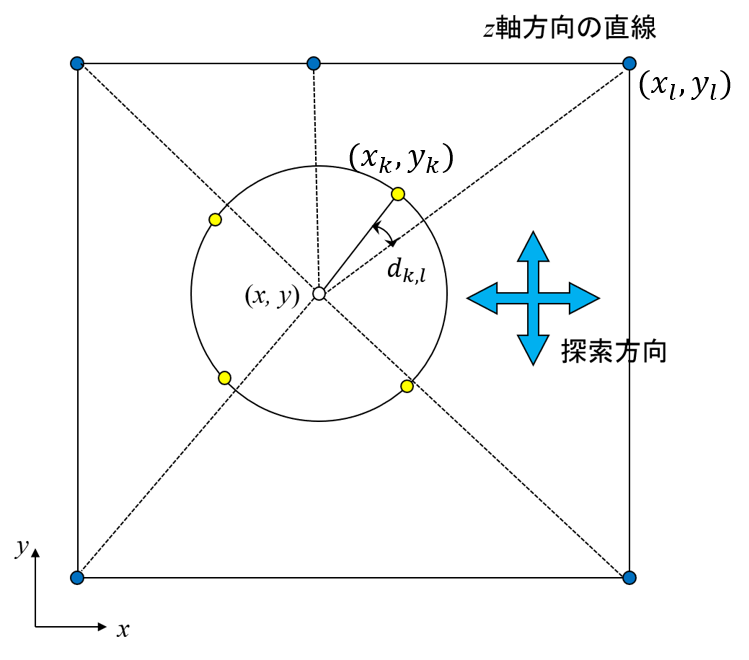
\includegraphics[width=0.6\columnwidth]{./chap4/fig/search_xy.png}
 \caption{座標$(x,y)$における全天球カメラを$z$軸方向から見た図}
 \label{fig:search_xy}
 \end{center}
\end{figure}


\clearpage
%==============================================================================
% 4.4
%==============================================================================
\section{$z$座標の推定}

$z$座標の推定では,$y$座標と前節で推定した$x$座標を固定し,1次元の最適化によって推定する.
まず,$xy$座標の推定と同様に,各交点$(x_k,z_k)$と$y$軸方向の直線の$xz$座標$(x_l,z_l)\ (l=1,2,...,m)$に対して以下の式で距離を計算する.

\begin{equation}
   d_{k,l} = \cos^{-1}\left(\frac{x_k(x_l-x^*)+z_k(z_l-z)}{\sqrt{(x_z-x^*)^2+(z_l-z)^2}}\right).
\end{equation}

$d_{k,l}\ (l=1,2,...,m)$のうち,最も小さいものを$d_k$とする.

\begin{equation}
   d_k = \min\left(d_{k,1},\ d_{k,2},\cdots,\ d_{k,m}\right).
\end{equation}

全ての交点における$d_k$の二乗和を最小とするようなパラメータ$(z^*)$が,$z$座標の推定値である.
この非線形最適化を,Levenberg-Marquardt法を用いて解く.

\begin{equation}
(z^*)=\argmin_{z} \sum_{k=1}^nd_k^2.
\label{eq:optim2}
\end{equation}


\begin{figure}[b]
 \begin{center}
 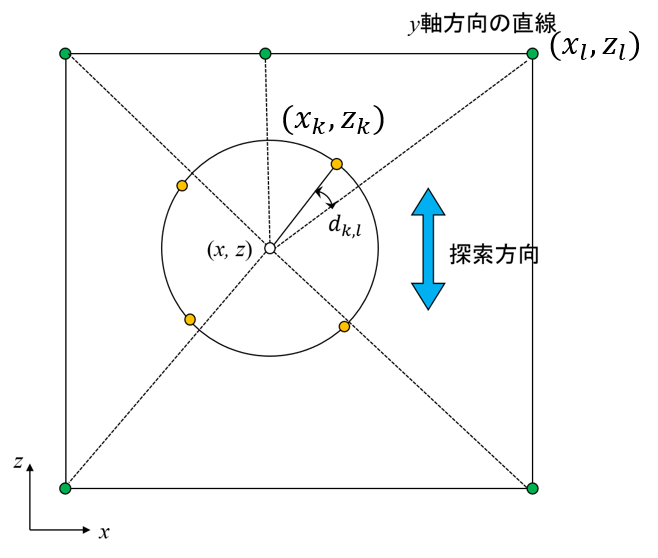
\includegraphics[width=0.6\columnwidth]{./chap4/fig/search_xz.png}
 \caption{座標$(x,z)$における全天球カメラを$y$軸方向から見た図}
 \label{fig:search_xz}
 \end{center}
\end{figure}


\clearpage
%==============================================================================
% 4.5
%==============================================================================
\section{おわりに}

本章では,位置推定手法について説明した.

4.2節にて,位置推定の概要を述べた.

4.3節にて,特徴量の計算について述べた.

4.4節にて,$xy$座標の推定方法について述べた.

4.5節にて,$z$座標の推定方法について述べる.


次章では,提案手法の有効性を検証するために行った実験について述べる.

\clearpage
%%%%%%%%%%%%%%%%%%%%%%%%%%%%%%%%%%%%%%%%%%%%%%%%%%%%%%%%%%%%%%%%%%%%%%%%%%%%%%%%%
%%%%% Local Variables:
%%%%% mode: katex
%%%%% TeX-master: "../thesis"
%%%%% End:

\chapter{実験による提案手法の評価}
\label{chap:development}
\minitoc

\thispagestyle{empty}

\newpage
%%%%%%%%%%%%%%%%%%%%%%%%%%%%%%%%%%%%%%%%%%%%%%%%%%%%%%%%%%%%%%%%%%%%%%%%%%%%%%%%%%%%%%%%%%%%%%%%%%%%%%%%%%%%%%%%%%%%%%%%%%%%%%%%%%%
\section{はじめに}
\label{sec:intro_chap5}

本章では,理学療法士の技能を利用した,起立動作の支援機器の設計と開発,ならびに評価実験について述べる.

\ref{sec:design_chap5}節にて,支援機器の設計について述べる.

\ref{sec:development_chap5}節にて,支援機器の開発について述べる.

\ref{sec:experiment_chap5}節にて,支援機器の評価を行った実験について述べる.

\ref{sec:outro_chap5}節にて,本章のまとめを述べる.

\textcolor{red}{改ページする予定です.}
%\clearpage
%%%%%%%%%%%%%%%%%%%%%%%%%%%%%%%%%%%%%%%%%%%%%%%%%%%%%%%%%%%%%%%%%%%%%%%%%%%%%%%%%%%%%%%%%%%%%%%%%%%%%%%%%%%%%%%%%%%%%%%%%%%%%%%%%%%
\section{支援機器の設計}
\label{sec:design_chap5}

本節では,起立動作の支援機器の設計について述べる.\\

\textcolor{red}{改ページする予定です.}
%\clearpage
%%%%%%%%%%%%%%%%%%%%%%%%%%%%%%%%%%%%%%%%%%%%%%%%%%%%%%%%%%%%%%%%%%%%%%%%%%%%%%%%%%%%%%%%%%%%%%%%%%%%%%%%%%%%%%%%%%%%%%%%%%%%%%%%%%%
\section{支援機器の開発}
\label{sec:development_chap5}

本節では,起立動作の支援機器の開発について述べる.\\

\textcolor{red}{改ページする予定です.}
%\clearpage
%%%%%%%%%%%%%%%%%%%%%%%%%%%%%%%%%%%%%%%%%%%%%%%%%%%%%%%%%%%%%%%%%%%%%%%%%%%%%%%%%%%%%%%%%%%%%%%%%%%%%%%%%%%%%%%%%%%%%%%%%%%%%%%%%%%
\section{評価実験}
\label{sec:experiment_chap5}

本節では,開発した支援機器の評価を行うための実験について述べる.\\

\textcolor{red}{改ページする予定です.}
%\clearpage
%%%%%%%%%%%%%%%%%%%%%%%%%%%%%%%%%%%%%%%%%%%%%%%%%%%%%%%%%%%%%%%%%%%%%%%%%%%%%%%%%%%%%%%%%%%%%%%%%%%%%%%%%%%%%%%%%%%%%%%%%%%%%%%%%%%

\section{おわりに}
\label{sec:outro_chap5}

本章では,理学療法士の技能を利用した,起立動作の支援機器の設計と開発,ならびに評価実験について述べる.

\ref{sec:design_chap5}節にて,支援機器の設計について述べた.

\ref{sec:development_chap5}節にて,支援機器の開発について述べた.

\ref{sec:experiment_chap5}節にて,支援機器の評価を行った実験について述べた.\\

開発した支援機器により健常な高齢者の起立動作を支援することが可能であることを確認した.

\clearpage
%%%%%%%%%%%%%%%%%%%%%%%%%%%%%%%%%%%%%%%%%%%%%%%%%%%%%%%%%%%%%%%%%%%%%%%%%%%%%%%%%%%%%%%%%%%%%%%%%%%%%%%%%%%%%%%%%%%%%%%%%%%%%%%%%%%
%%% Local Variables:
%%% mode: katex
%%% TeX-master: "../thesis"
%%% End:

\chapter{結論}
\thispagestyle{empty}
\label{chap6}
\minitoc

\newpage
%%%%%%%%%%%%%%%%%%%%%%%%%%%%%%%%%%%%%%%%%%%%%%%%%%%%%%%%%%%%%%%%%%%%%%%%%%%%%%%
%==============================================================================
%まとめ
%==============================================================================
\section{結論}

本論文では,直線情報に基づく全天球カメラの高速な6自由度の位置姿勢推定手法を提案した.
\vspace{\baselineskip}

第1章にて,研究背景として位置姿勢推定における全天球カメラの優位性を示し,関連する従来研究では,大域的アプローチによる全天球カメラの6自由度の位置姿勢推定として,リアルタイムのアプリケーションに適用できるような高速な手法は提案されていないことを述べた.これに基づき本研究の目的を「全天球カメラを用いた大域的なアプローチによる高速な6自由度の位置姿勢推定」と設定した.
\vspace{\baselineskip}

第2章において,本研究のアプローチについて述べた.
本研究では,位置姿勢推定において位置の推定と姿勢の推定を分離して行い,初めに姿勢を推定してから位置を推定することを述べた.
姿勢推定は消失点を用いて行い,画像の勾配のみから推定することで高速化することを述べた.
位置推定は,$xy$座標の推定と$z$座標の推定を分離してそれぞれを高速に行うことを述べた.
\vspace{\baselineskip}

第3章では姿勢推定の提案手法について詳しく説明した.
姿勢推定は,単位球面勾配ベクトルの分布とマンハッタンワールドにおける互いに直交する3平面を比較することによって行うことを説明した.
単位球面勾配ベクトルの計算は,画像内の2次元の勾配ベクトルを変換することによって行い,歪みによる勾配の計算精度の低下を抑えるために,歪みの大きい領域における勾配の計算には,入力画像を球面に変換して3次元空間において回転させた画像を用いることを述べた.
\vspace{\baselineskip}

第4章では位置推定の提案手法について詳しく説明した.
$z$軸方向に伸びる直線が投影された球上の直線と全天球カメラの$xy$平面の交点の分布は,カメラの$xy$座標にのみ依存することから,これを利用してまず$xy$座標を推定することを述べた.
その後,$x$軸方向に伸びる直線が投影された球上の直線と全天球カメラの$yz$平面の交点の分布を利用して$z$座標を推定する手法を提案した.
\vspace{\baselineskip}

第5章では,提案手法の有効性を示すために行った実験について述べた.
シミュレーション環境および実環境において位置姿勢推定実験を行い,高速に推定可能であることを実証した.
一方で,推定精度に関しては改善の必要があることが確認された.
\vspace{\baselineskip}

本論文により,直線情報に基づく全天球カメラの高速な6自由度の位置姿勢推定手法が確立された.

\newpage
%==============================================================================
%今後の展望
%==============================================================================
\section{今後の展望}

本論文では,直線情報に基づく全天球カメラの高速な6自由度の位置姿勢推定手法を構築した.
位置姿勢を高速に推定することができたものの,推定精度に関しては課題が残る結果となった.
さらなる性能の向上のためには,直線以外の情報の活用が考えられる.
例えば,直線周辺のテクスチャ情報を利用することなどが例として挙げられる.
これにより,精度やロバスト性の向上が期待される.
\vspace{\baselineskip}

%また,本手法は大域的アプローチによって全天球カメラの位置姿勢推定を行った.環境全域からある程度の位置を推定することができれば全天球カメラ画像と3次元モデルの直線の対応を推定することができる.直線の対応を推定できれば,直線の対応を用いて位置姿勢を推定することでより高精度に位置姿勢推定が可能となる.
%\vspace{\baselineskip}

また,本手法で使用した変数や閾値の中には試行錯誤的に定められたものが数点存在する.
環境によっては,これらのパラメータが精度に影響を与えることも考えられる.
特に,エッジ検出のパラメータは直線検出の精度に大きな影響を与える可能性があり,環境によって適切に定める必要がある.
従って,これらのパラメータを適切に決定する手法の構築は本手法の実用化において必要な課題である.
\vspace{\baselineskip}

%また,本手法では屋内環境に着目した手法を提案したが,様々な用途に対応するためには屋外環境にも適用可能な手法の構築が必要となる.
%屋外環境では,日照条件の違いによる照明の変化や車などの移動物体など,屋内環境にはない課題が考えられる.
%これらの課題を克服するために,屋外環境に対応可能なディスクリプタの構築が必要となる.
%\vspace{\baselineskip}

このような課題を解決することで,本提案手法は全天球カメラの位置姿勢推定を行う際の一般的枠組みとして幅広く応用可能になることが期待できる.


\newpage

%%%%%%%%%%%%%%%%%%%%%%%%%%%%%%%%%%%%%%%%%%%%%%%%%%%%%%%%%%%%%%%%%%%%%%%%%%%%%%%%
%%%% Local Variables:
%%%% mode: katex
%%%% TeX-master: "../thesis"
%%%% End:

\cleardoublepage
}

%
%謝辞
\addcontentsline{toc}{chapter}{謝辞}
\chapter*{謝辞}
\thispagestyle{empty}
\markboth{謝辞}{}
\label{thankyou}
%\def\thepage{}

\newpage

本論文は筆者が東京大学大学院 工学系研究科 精密工学専攻 山下研究室在籍中の研究の成果をまとめ,多くの方々にご指導ご協力をいただいて執筆されたものです.
本論文の締めくくりに,この場を借りて以下に感謝の意を表します.\\

はじめに本研究の指導教員である東京大学大学院 工学系研究科 精密工学専攻准教授 山下 淳先生には,有意義な研究の機会を与えていただき,また多くのことをご教示いただきました.
研究の方向性,取り組み方,研究発表の仕方や論文の添削と細部にわたってご指導いただきました.
ここに深く感謝申し上げます.
博士課程においても,ご指導ご鞭撻のほどよろしくお願いいたします.
\\

東京大学大学院 工学系研究科 精密工学専攻教授 太田 順先生,准教授 原 辰徳先生には本研究の副査を引き受けていただきました.
自分の研究に対する問いやその答えに至るまでの考え方など,本論文についてたくさんの貴重なご意見をいただきました.
ここに深謝の意を表します.\\

東京大学大学院 工学系研究科 精密工学専攻教授 淺間 一先生には,ご多忙の中でグループミーティングや発表練習でご指導ご鞭撻を賜りました.
さらに,一ヶ月半に亘るドイツへの留学の機会を与えてくださいました.博士課程への進学について深く考える契機となり,今後の研究生活において非常に有意義な時間であったと確信しております.
ここに拝謝の意を表します.
博士課程で淺間先生に直接ご指導いただけることを光栄に思います.
\\

東京大学大学院 工学系研究科 精密工学専攻特任准教授 田村 雄介先生には,グループミーティングや論文の添削で多くの有意義なコメントをいただきました.
また,廃炉に関してイギリスや青森への視察の機会も与えてくださり,自分の見識を拡げることができました.
心から感謝申し上げます.\\

東京大学大学院 工学系研究科 精密工学専攻助教 安 琪先生には,研究についてのアドバイスだけでなく,研究に対する心構えや様々な知識をご教示いただきました.
産まれたての溺愛する娘との時間を割いてまで発表資料や論文の添削を賜ることもありました.
また,国内外問わず自分の行く全ての学会にも同行してくださりました.
心から感謝申し上げます.\\

東京大学大学院 工学系研究科 精密工学専攻技術専門員 山川 博司先生には,電子回路や機械設計への知識の造詣の深さから,機器開発のサポートをしていただきました.
山川先生のご尽力により機器の開発まで進めることができました.
心から感謝申し上げます.\\

理化学研究所 脳神経科学研究センター 下田 真吾先生,山崎 弘嗣先生,Fady Shibata-Alnajjar先生,Matti Itkonen先生,園尾 萌香さんには大阪の森之宮病院における計測実験や自分の研究に関するアドバイスをしていただきました.
皆様と大阪で過ごした時間はとても有意義なものでした.
深く感謝申し上げます.\\

森之宮病院 宮井 一郎先生,服部憲明先生,乙宗 宏範先生,木野本 誠さん,高橋 幸治さん,藤井 崇典さん,奥田 陽子さん,三矢田 美佐子さんには大阪の森之宮病院における計測実験に協力いただきました.
患者さんのリクルートや自分の研究へのご助言をしていただきました.
深く感謝申し上げます.\\

東京大学大学院 工学系研究科 精密工学専攻 特任准教授 温 文先生には,発表練習やグループミーティングにおいてご指導・ご助言をいただきました.
深く感謝いたします.\\

東京大学大学院 工学系研究科 精密工学専攻 特任研究員 濱崎 峻資先生には,発表練習やグループミーティングにおいてご指導・ご助言をいただきました.
また,普段の研究生活においても相談に乗っていただきました.
深く感謝いたします.\\

東京大学大学院 工学系研究科 精密工学専攻 特任研究員 Sarthak Pathak先生には,発表練習で的確なご助言やMatlabのサーバに関する相談にも乗っていただきました.
また,お酒の席で楽しい時間を過ごさせていただきました.
深く感謝いたします.\\

東京大学大学院 工学系研究科 精密工学専攻 特任研究員 禹 ハンウル先生には,発表練習の場でご指導・ご助言いただきました.
また,お酒の席で様々なことについて談笑させていただきました.
深く感謝いたします.\\

東京大学大学院 工学系研究科 精密工学専攻 特任研究員 淵田 正隆先生には,発表練習の場でご指摘・ご質問をいただきました.
深く感謝いたします.\\

東京大学大学院 工学系研究科 精密工学専攻 特任研究員 Angela Faragasso先生には,発表練習の場でご指摘・ご質問いただきました.
また,ICRAやEmboSSに参加した際には談笑をして,楽しい時間を過ごさせていただきました.
深く感謝申し上げます.\\

東京大学大学院 工学系研究科 精密工学専攻 特任研究員 Renato Miyagusuku先生には,発表練習の場で的確なご指導・ご助言いただきました.
また,研究室のネットワークの問題にも一緒に対応をしてくださりました.
深く感謝申し上げます.\\

千葉工業大学 先進工学部 未来ロボティクス学科 准教授 藤井 浩光先生には,1年間という短い時間でしたが,発表練習の場でご指摘・ご質問をいただきました.
また,研究室内のサーバやネットワークに関することで幾度となくご助言をいただきました.
深く感謝申し上げます.\\

研究室の先輩の皆様には,発表練習や普段の研究室生活において大変お世話になりました.
先輩方の研究に対する姿勢をいつもお手本にさせていただきました.
特に同じグループの楊 寧嘉氏には実験の手伝いや解析を手伝っていただました.
大変感謝いたします.\\

研究室の同期である青柳 恵さん,奥村 有加里さん,杉本 賢勇君,森山 湧志君とは,普段の雑談から始まり講義や研究について様々なことを相談しました.
お互いに苦楽を共有し,分かち合いつつも切磋琢磨することで大きく成長することができました.
この二年間はかけがえのない財産となりました.ありがとうございました.\\

研究室の後輩の皆様には,日頃の研究室生活から大変お世話になりました.
皆さまが研究に熱心に取り組んでいる姿は自分にとって良い刺激になりました.
特に自分と同じ部屋にいた川田 桃子さん,長野 樹君,尹 碩珉君とは愉快な時間を過ごさせていただきました.
大変感謝いたします.\\

秘書の成島 久恵さん,中村 恵さん,小島 里佳さん,後藤田 彩さん,石田 万紀さんには,研究室生活におけるあらゆる面で支えていただきました.
学会や出張時の費用の申請や,購入した物品の費用の手続き,その他煩わしい事務作業をすべて引き受けていただきました.
出張のたびに皆さんにお土産を喜んでいただけましたので,お土産を選ぶ時間は楽しいひと時でした.
集中して研究できたのも秘書の皆様のおかげです.
深く感謝申し上げます.\\

そして,大学院への進学の機会を与えてくださり,いつも自分を支えてくださった家族に深く感謝の意を表します.

最後に,お世話になったすべての人に改めて深く感謝いたします.本当にありがとうございました.


\begin{flushright}
平成30年2月吉日 湖上碩樹
\end{flushright}

\newpage
%%%%%%%%%%%%%%%%%%%%%%%%%%%%%%%%%%%%%%%%%%%%%%%%%%%%%%%%%%%%%%%%%%%%%%%%%%%%%%%

%%%%%%%%%%%%%%%%%%%%%%%%%%%%%%%%%%%%%%%%%%%%%%%%%%%%%%%%%%%%%%%%%%%%%%%%%%%%%%%
%%% Local Variables:
%%% mode: katex
%%% TeX-master: "../thesis"
%%% End:

\cleardoublepage
	
%参考文献
\bibliographystyle{junsrt}
\bibliography{ref}
\addcontentsline{toc}{chapter}{参考文献}
\chapter*{参考文献}
%\addcontentsline{toc}{chapter}{参考文献}
\lhead[参考文献]{}
%\renewcommand{\refname}{引用文献}
\thispagestyle{empty}

\newpage

%==============================================================================
%和文文献
%==============================================================================
\subsection*{\textmc{<和文文献>}}
\begin{mythebibliography}{}

\bibitem[伊部 2015]{伊部2015}
\leavevmode \\伊部~公紀, 小林~祐一, 金子~透, 山下~淳:
\newblock ``複光路単眼ステレオによる直方体容器中の水中物体の3次元計測'',
\newblock 精密工学会誌, Vol.~81, No.~12, pp.~1093--1101, 2015.
\\

\bibitem[内山 2014]{内山2014}
\leavevmode \\内山~庄一郎, 井上~公, 鈴木~比奈子:
\newblock ``SfM を用いた三次元モデルの生成と災害調査への活用可能性に関する研究'',
\newblock 防災科学技術研究所研究報告, Vol.~81, pp.~37--60, 2014.
\\

\bibitem[内山 2017]{内山2017}
\leavevmode \\内山~庄一郎, 鈴木~比奈子, 中村~一樹, 上石~勲:
\newblock ``無人航空機とSfM写真測量による2017年3月27日栃木県那須町の雪崩災害調査'',
\newblock 雪氷研究大会, p.~74, 2017.
\\

\bibitem[岡谷 2009]{岡谷2009}
\leavevmode \\岡谷貴之:
\newblock ``バンドルアジャストメント'',
\newblock 情報処理学会研究報告 No.~2009-CVIM-167, Vol.~37, \mbox{pp.~1--16}, 2009.
\\

\bibitem[奥村 2017]{奥村2017}
\leavevmode \\奥村~有加里, 藤井~浩光, 山下~淳, 淺間~一:
\newblock ``屈折を利用したスケール復元が可能な計測誤差に頑健なStructure from Motion'',
\newblock 精密工学会誌, Vol.~83, No.~12, pp. 1201--1208, 2017.
\\

\bibitem[小花和 2014]{小花和2014}
\leavevmode \\小花和~宏之, 早川~裕弌, ゴメス~クリストファー:
\newblock``UAV空撮とSfMを用いたアクセス困難地の3Dモデリング",
\newblock 地形, Vol.~35, No.~3, pp.~283--294, 2014. 
\\

\bibitem[金谷 2000]{金谷2001}
\leavevmode \\金谷~健一, 三島~等:
\newblock ``未校正カメラによる2画像からの3次元復元とその信頼性の評価'',
%\newblock 情報処理学会論文誌:コンピュータビジョンとイメージメディア, Vol.~42, No.~SIG~6, pp.~1--8, 2001.
\newblock 情報処理学会研究報告, No.~33, pp.~25--32, 2000.
\\

\newpage

\bibitem[川西 2012]{川西2012}
\leavevmode \\川西~亮輔, 山下~淳, 金子~透:
\newblock ``全方位画像中の特徴点と直線エッジの同時拘束と基線長の自動決定に基づくStructure from Motionによる三次元環境モデル生成'',
\newblock 日本ロボット学会誌, Vol.~30, No.~4, pp.~399--410, 2012.
\\

\bibitem[延原 2016]{延原2016}
\leavevmode \\延原~肇:
\newblock ``農作物を対象にしたUAVによる時空間アーカイビング'',
\newblock 日本ロボット学会誌, Vol.~34, No.~2, pp.~123--126, 2016.
\\

\bibitem[山田 2009]{山田2009}
\leavevmode \\山田~健人, 金澤~靖, 金谷~健一, 菅谷~保之:
\newblock ``2画像からの3次元復元の最新アルゴリズム'',
\newblock 情報処理学会研究報告, No.~3, pp.~1--8, 2009.
\\

\bibitem[日本写真測量学会 2016]{三次元画像計測の基礎}
\leavevmode \\一般社団法人 日本写真測量学会 (編):
\newblock 三次元画像計測の基礎--バンドル調整の理論と実践--,
\newblock 東京電機大学出版局, 2016.
\\

\bibitem[化学便覧]{化学便覧}
\leavevmode \\岩澤 康裕一 (編):
\newblock 化学便覧 基礎編I\hspace{-.1em}I 改訂5版,
\newblock 丸善出版, pp.~643, 2004.
\\

%\bibitem[岩元 2011]{岩元2011}
%\leavevmode \\岩元祐輝, 菅谷保之, 金谷健一:
%\newblock ``3次元復元のためのバンドル調整の実装と評価'',
%\newblock 情報処理学会研究報告 2011-CVIM-175(19), pp.~1--8, 2011.
%\\
%
%

%
%\bibitem[金出 1993]{金出1993}
%\leavevmode \\金出武雄, コンラッド ポールマン, 森田俊彦:
%\newblock ``因子分解法による物体形状とカメラ運動の復元'',
%\newblock 電子情報通信学会論文誌, Vol.~J76-D-2, No.~8, pp.~1497--1505, 1993.
%\\
%

%
%\bibitem[久米 2014]{久米2014}
%\leavevmode \\久米大将, 藤井浩光, 山下淳, 淺間一:
%\newblock ``全方位カメラを用いたスケール復元が可能な水中Structure from Motion'',
%\newblock 2014年度精密工学会春季大会学術講演会講演論文集, \mbox{pp.~981--982}, 2014.
%\\
%
%\bibitem[松井 2010]{松井2010}
%\leavevmode \\松井建樹, 山下淳, 金子透:
%\newblock ``全方位レーザ・全方位カメラからなるレンジファインダの自己位置推定と配管の3次元モデル生成'',
%\newblock 電気学会論文誌C, Vol.~130, No.~9, pp.~1504--1512, 2010.
%\\
%
%\bibitem[松久 2008]{松久2008}
%\leavevmode \\松久亮太, 川崎洋, 小野晋太郎, 阪野貴彦, 池内克史:
%\newblock ``因子分解法とバンドル調整による全方位画像列からの形状および位置姿勢の同時推定手法'',
%\newblock 画像の認識・理解シンポジウム(MIRU2008), pp.~1610--1617, 2008.
%\\
%

%
%\bibitem[東京電力株式会社 HP]{東京電力株式会社HP}
%\leavevmode \\東京電力株式会社:
%\newblock 福島第一原発原子炉建屋周辺の様子(画像),\\
%\newblock http://photo.tepco.co.jp/cat2/01-j.html, 2014.
%\\



\newpage
%==============================================================================
%英文文献
%==============================================================================
\subsection*{\textmc{\hspace{-1zw}<英文文献>}}

\bibitem[Agrawal 2012]{Agrawal2012} 
\leavevmode \\Amit Agrawal, Srikumar Ramalingam, Yuichi Taguchi and Visesh Chari:
\newblock ``A Theory of Multi-Layer Flat Refractive Geometry'',
\newblock Proceedings of the 2012 IEEE Conference on Computer Vision and Pattern Recognition, pp.~2316--2323, 2012.
\\

\bibitem[Alcantarilla 2012]{Alcantarilla2012} 
\leavevmode \\Pablo Fernandez Alcantarilla, Adrien Bartoli and Andrew J. Davison:
\newblock ``KAZE Features'',
\newblock Proceedings of the 2012 European Conference on Computer Vision, pp.~214--227, 2012.
\\


\bibitem[Bay 2008]{Bay2008}
\leavevmode \\Herbert Bay, Andreas Ess, Tinne Tuytelaars and Luc Van Gool:
\newblock ``Speeded-Up Robust Features (SURF)'',
\newblock Computer Vision and Image Understanding, Vol.~110, No.~3, pp.~346--359, 2008.
\\

\bibitem[Chen 2011]{Chen2011} 
\leavevmode \\Zhihu Chen, Kwan-Yee K. Wong, Yasuyuki Matsushita, Xiaolong Zhu and Miaomiao Liu:
\newblock ``Self--Calibrating Depth from Refraction'',
\newblock Proceedings of the 2011 IEEE International Conference on Computer Vision, pp.~635--642, 2011.
\\

\bibitem[Chadebecq 2017]{Chadebecq2017} 
\leavevmode \\François Chadebecq, Francisco Vasconcelos, George Dwyer, Rene Lacher, Sebastien Ourselin, Tom Vercauteren and Danail Stoyanov:
\newblock ``Refractive Structure-from-Motion Through a Flat Refractive Interface'',
\newblock Proceedings of the 2017 IEEE International Conference on Computer Vision, pp.~5325--5333, 2017.
\\

\bibitem[Feng 2015]{Feng2015}
\leavevmode \\Xiao-feng Feng and Di-fu pan:
\newblock ``Research on the Application of Single Stereo Vision Sensor in Three-Dimensional Point Measurement'',
\newblock Journal of Modern Optics, Vol.~62, No.~15, pp.~1204--1210, 2015.
\\

\bibitem[Fischler 1981]{Fischler1981}
\leavevmode \\Martin A. Fischler and Robert C. Bolles:
\newblock ``Random Sample Consensus: a Paradigm for Model Fitting with Applications to Image Analysis and Automated Cartography'',
\newblock Communications of the ACM, Vol.~24, No.~6, pp.~381--395, 1981.
\\

\bibitem[Gao 2006]{Gao2006} 
\leavevmode \\Chunyu Gao and Narendra Ahuja:
\newblock ``A Refractive Camera for Acquiring Stereo and Super--resolution Images'',
\newblock Proceedings of the 2006 IEEE Computer Society Conference on Computer Vision and Pattern Recognition, pp.~2316--2323, 2006.
\\

\bibitem[Gluckman 1999]{Gluckman1999}
\leavevmode \\Joshua Gluckman and Shree K. Nayer:
\newblock ``Planar Catadioptric Stereo: Geometry and Calibration'',
\newblock  Proceedings of the 1999 IEEE Computer Society Conference on Computer Vision and Pattern Recognition, pp.~22--28, 1999.
\\

\bibitem[Grater 2015]{Grater2015} 
\leavevmode \\Johannes Grater, Tobias Schwarze and Martin Lauer:
\newblock ``Robust Scale Estimation for Monocular Visual Odometry Using Structure from Motion and Vanishing Points'',
\newblock Proceedings of the 2015 IEEE Intelligent Vehicles Symposium, pp.475--480, 2015.
\\

\bibitem[Hartley 1997]{Hartley1997}
\leavevmode \\Richard I. Hartley:
\newblock ``In Defense of the Eight-Point Algorithm'',
\newblock IEEE Transactions on Pattern Analysis and Machine Intelligence, Vol.~19, No.~6, pp.~580--593, 1997.
\\

\bibitem[Hartley 2004]{Hartley2004} 
\leavevmode \\Richard I. Hartley and Andrew Zisserman:
\newblock Multiple View Geometry in Computer Vision,
\newblock Cambridge University Press, Second Edition, 2004.
\\

\bibitem[Huang 2014]{Huang2014} 
\leavevmode \\Longxiang Huang and Yuncai Liu:
\newblock ``Camera Calibration for Plate Refractive Imaging System'',
\newblock Proceedings of the 2014 22nd International Conference on Pattern Recognition, pp.~4068--4073, 2014.
\\



\bibitem[Jordt-Sedlazeck 2013]{Jordt-Sedlazeck2013}
\leavevmode \\Anne Jordt-Sedlazeck and Reinhard Koch:
\newblock ``Refractive Structure--from--Motion on Underwater Images'',
\newblock Proceedings of the 2013 IEEE International Conference on Computer Vision, \\pp.~57--64, 2013.
\\



\bibitem[Jordt 2016]{Jordt2016}
\leavevmode \\Anne Jordt, Kevin Koser and Reinhard Koch:
\newblock ``Refractive 3D Reconstruction on Underwater Images'',
\newblock Methods in Oceanography, pp.~90--113, 2016.
\\

\bibitem[Longuet-Higgins 1981]{Longuet-Higgins1981}
\leavevmode \\H. C. Longuet-Higgins:
\newblock ``A Computer Algorithm for Reconstructing a Scene from Two Projections'',
\newblock Nature, Vol.~293, pp.~133--135, 1981.
\\

\bibitem[Lourakis 2013]{Lourakis2013} 
\leavevmode \\Manolis Lourakis and Xenophon Zabulis:
\newblock ``Accurate Scale Factor Estimation in 3D Reconstruction'',
\newblock Proceedings of the International Conference on Computer Analysis of Images and Patterns, Vol.~1, pp.498--506, 2013.
\\

\bibitem[Lowe 2004]{Lowe2004}
\leavevmode \\Daved G. Lowe:
\newblock ``Distinctive Image Features from Scale-Invariant Keypoints'',
\newblock International Journal of Computer Vision, Vol.~60, No.~2, pp.~91--110, 2004.
\\

\bibitem[Murray 2000]{Murray2000}
\leavevmode \\Don Murray and James J. Little:
\newblock ``Using Real-Time Stereo Vision for Mobile Robot Navigation'',
\newblock Autonomous Robots, Vol.~8, No.~2, pp.~161--171, 2000.
\\

\bibitem[Nister 2004]{Nister2004}
\leavevmode \\David Nister:
\newblock ``An Efficient Solution to the Five-Point Relative Pose Problem'',
\newblock IEEE Transactions on Pattern Analysis and Machine Intelligence, Vol.~26, No.~6, pp.~756--770, 2004.
\\

\newpage

\bibitem[Scaramuzza 2009]{Scaramuzza2009}
\leavevmode \\Davide Scaramuzza, Friedrich Fraundorfer, Marc Pollefeys and Roland Siegwart:
\newblock ``Absolute Scale in Structure from Motion from a Single Vehicle Mounted Camera by Exploiting Nonholonomic Constraints'',
\newblock Proceedings of the 2009 IEEE International Conference on Computer Vision, pp.~1413--1419, 2009.
\\



\bibitem[Shibata 2015a]{shibata2015a}
\leavevmode \\Akira~Shibata, Hiromitsu~Fujii, Atsushi~Yamashita and Hajime~Asama:
\newblock``Scale-Reconstructable Structure from Motion Using Refraction with a Single Camera",
\newblock Proceedings of the 2015 IEEE International Conference on Robotics and Automation, pp.~5239--5244, 2015.
\\

\bibitem[Shibata 2015b]{shibata2015b}
\leavevmode \\Akira~Shibata, Hiromitsu~Fujii, Atsushi~Yamashita and Hajime~Asama:
\newblock``Absolute Scale Structure from Motion Using a Refractive Plate",
\newblock Proceedings of the 2015 IEEE/SICE International Symposium on System Integration, pp.~540--545, 2015.
\\

\bibitem[Shibata 2018]{shibata2018}
\leavevmode \\Akira~Shibata, Yukari~Okumura, Hiromitsu~Fujii, Atsushi~Yamashita and Hajime~Asama:
\newblock``Refraction-based Bundle Adjustment for Scale Reconstructible Structure from Motion",
\newblock Journal of Robotics and Mechatronics, Vol.~30, No.~4, pp.~660--670, 2018.
\\

\bibitem[Triggs 2000]{Triggs2000}
\leavevmode \\Bill Triggs, Philip F. McLauchlan, Richard I. Hartley and Andrew W. Fitzgibbon:
\newblock ``Bundle Adjustment -- A Modern Synthesis'',
\newblock Vision Algorithms: Theory and Practice, pp.~298--372, 2000.
\\

\bibitem[Ummenhofer 2017]{Ummenhofer2017}
\leavevmode \\Benjamin~Ummenhofer, Huizhong~Zhou, Jonas~Uhrig, Nikolaus~Mayer, Eddy~Ilg, Alexey~Dosovitskiy and Thomas~Brox:
\newblock``DeMoN: Depth and Motion Network for Learning Monocular Stereo",
\newblock Proceedings of the 2017 IEEE International Conference on Computer Vision and Pattern Recognition, pp.~5038--5047, 2017.
\\



\bibitem[Zhang 2000]{Zhang2000}
\leavevmode \\Zhengyou Zhang:
\newblock ``A Flexible New Technique for Camera Calibration'',
\newblock IEEE Transactions on Pattern Analysis and Machine Intelligence, Vol.~22, No.~11, pp. 1330--1334, 2000.
\\

%\bibitem[Agarwal 2009]{Agarwal2009} 
%\leavevmode \\Sameer Agarwal, Noah Snavely, Ian Simon, Steven M. Seitz and Richard Szeliski:
%\newblock ``Building Rome in a Day'',
%\newblock Proceedings of the 2009 IEEE International Conference on Computer Vision, pp.~72--79, 2009.
%\\

%
%\bibitem[Chang 2011]{Chang2011}
%\leavevmode \\Yao-Jen Chang and Tsuhan Chen:
%\newblock ``Multi-View 3D Reconstruction for Scenes under the Refractive Plane with Known Vertical Direction'',
%\newblock Proceedings of the 2011 IEEE International Conference on Computer Vision, pp.~351--358, 2011.
%\\

%
%\newpage
%


%
%
%\bibitem[Kukelova 2011]{Kukelova2011}
%\leavevmode \\Zuzana Kukelova, Martin Bujnak and Tomas Pajdla:
%\newblock ``Closed-form solutions to the minimal absolute pose problems with known vertical direction'',
%\newblock Proceedings of the Asian Conference on Computer Vision, pp.~216--229, 2010.
%\\
%
%\bibitem[Lee 1999]{Lee1999} 
%\leavevmode \\Doo Hyun Lee, In So Kweon and Roberto Cipolla:
%\newblock ``A Biprism--Stereo Camera System'',
%\newblock Proceedings of the 1991 IEEE Computer Society Conference on Computer Vision and Pattern Recognition, Vol.~1, pp.~82--87, 1999.
%\\
%

%
%\bibitem[Snavely 2006]{Snavely2006}
%\leavevmode \\Noah Snavely, Steven M. Seitz and Richard Szeliski:
%\newblock ``Photo Tourism: Exploring Photo Collections in 3D'',
%\newblock ACM Transactions on Graphics, Vol.~25, pp. 835--846 , 2006.
%\\
%
%\bibitem[Tomasi 1992]{Tomasi1992}
%\leavevmode \\Carlo Tomasi and Takeo Kanade:
%\newblock ``Shape and Motion from Image Streams under Orthography: a Factorization Method'',
%\newblock International Journal of Computer Vision, Vol.~9, No.~2, pp.~137--154, 1992.
%\\
%
%\bibitem[Treibitz 2011]{Treibitz2011}
%\leavevmode \\Tali Treibitz, Yoav Y. Schechner and Hanumant Singh:
%\newblock ``Flat Refractive Geometry'',
%\newblock IEEE Transactions on Pattern Analysis and Machine Intelligence, Vol.~34, No.~1, pp.~51--65, 2011.
%\\
%

%\bibitem[Yamashita 2010]{Yamashita2010} 
%\leavevmode \\Atsushi Yamashita, Yudai Shirane and Toru Kaneko:
%\newblock ``Monocular Underwater Stereo -- 3D Measurement Using Difference of Appearance Depending on Optical Paths --'',
%\newblock Proceedings of the 2010 IEEE/RSJ International Conference on Intelligent Robots and Systems, pp.~3652--3657, 2010.
%\\
%
%\newpage
%
%\bibitem[Yamashita 2011]{Yamashita2011}
%\leavevmode \\Atsushi Yamashita, Kenki Matsui, Ryosuke Kawanishi, Toru Kaneko, Taro Murakami, Hayato Omori, Taro Nakamura and Hajime Asama:
%\newblock ``Self-Localization and 3-D Model Construction of Pipe by Earthworm Robot Equipped with Omni-Directional Rangefinder'',
%\newblock Proceedings of the 2011 IEEE International Conference on Robotics and Biomimetics, \mbox{pp.~1017--1023}, 2011.
%\\
%






%scale problem
%・Accurate Scale Factor Estimation in 3D Reconstruction
%\bibitem{4} Manolis Lourakis and Xenophon Zabulis: ``Accurate Scale Factor Estimation
%in 3D Reconstruction'',
%{\it Proceedings of the International Conference on Computer Analysis of Images and Patterns}, 
%Vol.1, pp.498--506, 2013.


%Plate calib
%・A Theory of Multi-Layer Flat Refractive Geometry
%Amit Agrawal, Srikumar Ramalingam, Yuichi Taguchi, Visesh Chari:
%Proceedings of the 2012 IEEE Conference on Computer Vision and Pattern Recognition, pp.~2316--2323, 2006.


%・Flat Refractive Geometry
%\bibitem{5} Tali Treibitz, Yoav Y. Schechner and Hanumant Singh: ``Flat Refractive
%Geometry'', 
%IEEE Transactions on Pattern Analysis and Machine Intelligence, Vol.~34, No.~1, pp.~51--65, 2011.


%with IMU 
%・Multi-View 3D Reconstruction for Scenes under the Refractive Plane with Known Vertical Direction
%\bibitem{13} Yao-Jen Chang and Tsuhan Chen: ``Multi-View 3D Reconstruction for Scenes under the Refractive Plane with Known Vertical Direction'',
%{\it Proceedings of the 2011 IEEE International Conference on Computer Vision}, 
%pp.351--358, 2011.

%・Closed-form solutions to the minimal absolute pose problems with known vertical direction
%Zuzana Kukelova, Martin Bujnak, Tomas Pajdla:
%Computer Vision -- ACCV 2010, pp.~216--229, 2011.

%with rangefinder
%・Self-Localization and 3-D Model Construction of Pipe by Earthworm Robot Equipped with Omni-Directional Rangefinder
%Atsushi Yamashita, Kenki Matsui, Ryosuke Kawanishi, Toru Kaneko, Taro Murakami, Hayato Omori, Taro Nakamura and Hajime Asama: "Self-Localization and 3-D Model Construction of Pipe by Earthworm Robot Equipped with Omni-Directional Rangefinder", Proceedings of the 2011 IEEE International Conference on Robotics and Biomimetics (ROBIO2011), pp.1017-1023, 2011.


%explain SfM 
%・Shape and Motion from Image Streams under Orthography: a Factorization Method 
%International Journal of Computer Vision, Vol.~9, No.~2, pp.~137--154, 1992 

%Bundle Adjustment -- A Modern Synthesis
%Bill Triggs, Philip F. McLauchlan, Richard I. Hartley, and Andrew W. Fitzgibbon:
%Vision Algorithms: Theory and Practice, pp.~298--372, 2000.

%absolute pose
%Absolute Pose for Cameras Under Flat Refractive Interfaces


\end{mythebibliography}
\cleardoublepage

%研究業績
\addcontentsline{toc}{chapter}{研究業績}
\chapter*{研究業績}
\thispagestyle{empty}
\markboth{研究業績}{}
\lhead[研究業績]{}
\label{achive}
%\def\thepage{}

\newpage
%==============================================================================
%査読有り学術論文投稿
%==============================================================================
\section*{査読有り学術論文}

\mbox{}
\begin{enumerate}[{[}1{]}]
\item \textbf{Hiroki Kogami}, Qi An, Ningia Yang, Hiroshi Yamakawa, Yusuke Tamura, Atsushi Yamashita, Hajime Asama, Shingo Shimoda, Hiroshi Yamasaki, Matti Itkonen, Fady Shibata-Alnajjar, Noriaki Hattori, Makoto Kinomoto, Kouji Takahashi, Takaori Fujii, Hironori Otomune and Ichiro Miyai: ``Effect of Physical Therapy on Muscle Synergy Structure During Standing-Up Motion of Hemiplegic Patients'', IEEE Robotics and Automation Letters (RA-L), Vol.~3, No.~3, pp.~2229--2236, 2018.
\end{enumerate}

%==============================================================================
%査読有り国際会議
%==============================================================================
\section*{査読有り国際会議}

\mbox{}
\begin{enumerate}[{[}1{]}]
\item \textbf{Hiroki Kogami}, Qi An, Ningia Yang, Hiroshi Yamakawa, Yusuke Tamura, Atsushi Yamashita, Hajime Asama, Shingo Shimoda, Hiroshi Yamasaki, Matti Itkonen, Fady Shibata-Alnajjar, Noriaki Hattori, Makoto Kinomoto, Kouji Takahashi, Takaori Fujii, Hironori Otomune and Ichiro Miyai: ``Effect of Physical Therapy on Muscle Synergy Structure During Standing-Up Motion of Hemiplegic Patients'', Proceedings of the IEEE International Conference on Robotics and Automation, pp.~1--8, Brisbane, Australia, 2018. 

\item \textbf{Hiroki Kogami}, Qi An, Ningia Yang, Hiroshi Yamakawa, Yusuke Tamura, Shingo Shimoda, Hiroshi Yamasaki, Matti Itkonen, Fady Shibata-Alnajjar, Noriaki Hattori, Makoto Kinomoto, Kouji Takahashi, Takaori Fujii, Hironori Otomune, Ichiro Miyai, Atsushi Yamashita and Hajime Asama: ``Effect of Physical Therapy on Joint Angle of Hemiplegic Patients during Standing-up Motion'', Proceedings of the 2nd International Symposium on Embodied-Brain Systems Science (EmboSS2018), pp.~1, Osaka, Japan, 2018. 
\end{enumerate}

\clearpage

%==============================================================================
%査読無し国内会議
%==============================================================================
\section*{査読無し国内会議}

\mbox{}
\begin{enumerate}[{[}1{]}]
\item \textbf{湖上 碩樹}, 安 琪, 楊 寧嘉, 山川 博司, 田村 雄介, 山下 淳, 淺間 一, 山崎 弘嗣, Matti Itkonen, Fady Shibata-Alnajjar, 下田 真吾, 服部 憲明, 木野本 誠, 藤井 崇典, 高橋 幸治, 乙宗 宏範, 宮井 一郎: ``片麻痺患者の起立動作のリハビリテーションにおける理学療法士の技能の解析'', 第23回創発システムシンポジウム講演資料, pp.~54, 茅野, 2017.

\item \textbf{湖上 碩樹}, 安 琪, 楊 寧嘉, 山川 博司, 田村 雄介, 山下 淳, 淺間 一, 山崎 弘嗣, Matti Itkonen, Fady Shibata-Alnajjar, 下田 真吾, 服部 憲明, 木野本 誠, 藤井 崇典, 高橋 幸治, 乙宗 宏範, 宮井 一郎: ``片麻痺患者の起立動作のリハビリテーションにおける理学療法士の技能の解析'', 計測自動制御学会システム・情報部門学術講演会予稿集, pp.~345--346, 浜松, 2017.

\item \textbf{湖上 碩樹}, 安 琪, 楊 寧嘉, 山川 博司, 田村 雄介, 山崎 弘嗣, Matti Itkonen, Fady Shibata-Alnajjar, 下田 真吾, 服部 憲明, 木野本 誠, 藤井 崇典, 高橋 幸治, 乙宗 宏範, 宮井 一郎, 山下 淳, 淺間 一: ``理学療法士の膝と臀部に対する介入が片麻痺患者の起立動作の身体軌道に与える影響の調査'', 計測自動制御学会システム・情報部門学術講演会予稿集, pp.~1--3, 富山, 2018.


\end{enumerate}

%%%%%%%%%%%%%%%%%%%%%%%%%%%%%%%%%%%%%%%%%%%%%%%%%%%%%%%%%%%%%%%%%%%%%%%%%%%%%%%

%%%%%%%%%%%%%%%%%%%%%%%%%%%%%%%%%%%%%%%%%%%%%%%%%%%%%%%%%%%%%%%%%%%%%%%%%%%%%%%
%%% Local Variables:
%%% mode: katex
%%% TeX-master: "../thesis"
%%% End:

\cleardoublepage
%
%
%%付録
%\appendix
%%\setcounter{page}{1}
%\renewcommand{\thechapter}{�t�^\Alph{chapter}}
%\renewcommand{\thechapter}{\Alph{chapter}}
%\renewcommand{\thepage}{\Alph{chapter}--\arabic{page}}
%\renewcommand{\thesection}{\Alph{chapter}.\arabic{section}}
%\renewcommand{\thesubsection}{\Alph{chapter}.\arabic{section}.\arabic{subsection}}
%\renewcommand{\furoku}[1]{\chapter{\thechapter\hspace{1.6zw}#1}}

%\furoku{�S�V���J�����̓����p�����[�^�ɂ‚���}
\chapter{�t�^A�@\, �S�V���J�����̓����p�����[�^�ɂ‚���}
%\chapter{ �t�^A�@\\ \vspace{10mm} �S�V���J�����̓����p�����[�^}
\lhead[�t�^\Alph{chapter}�@�S�V���J�����̓����p�����[�^�ɂ‚���]{}
\setcounter{page}{1}
\renewcommand{\thepage}{A--\arabic{page}}

\thispagestyle{empty}

\newpage
%%%%%%%%%%%%%%%%%%%%%%%%%%%%%%%%%%%%%%%%%%%%%%%%%%%%%%%%%%%%%%%%%%%%%%%%%%%%%%%
\section{�S�V���J�����̓����p�����[�^�̌���}

�{�����ŗp���Ă���S�V���J�����iRICOH�А�THETA S�j�́C�����Ɏ��t����2�‚̋���J������\�荇�킹�邱�Ƃɂ���ċ��̉摜�𐶐����Ă���C�^���̃��f���ɏ]���Ă���D�����p�����[�^�����f�����\���ɕ\���ł��Ȃ��ꍇ�ɂ́C�J�����摜���琶�������@���x�N�g����3�������f�����琶�������@���x�N�g���ƈ�v�����f�B�X�N���v�^�ɂ��}�b�`���O�����x�ǂ��s���Ȃ����Ƃ��\�z�����D�{�����ł́C�J�����̐��������񋟂�������p�����[�^�ɂ���Đ�������鐳���~���摜��p�����ꍇ�C���x�ǂ����̃��f���ɏ]�����Ƃ����O�Ɍ��؂��C�摜�ɂ͓����p�����[�^�̂���ɂ��c�݂͂Ȃ����̂Ƃ��ėp���Ă���D\\

\begin{figure}[b]
	\begin{center}
		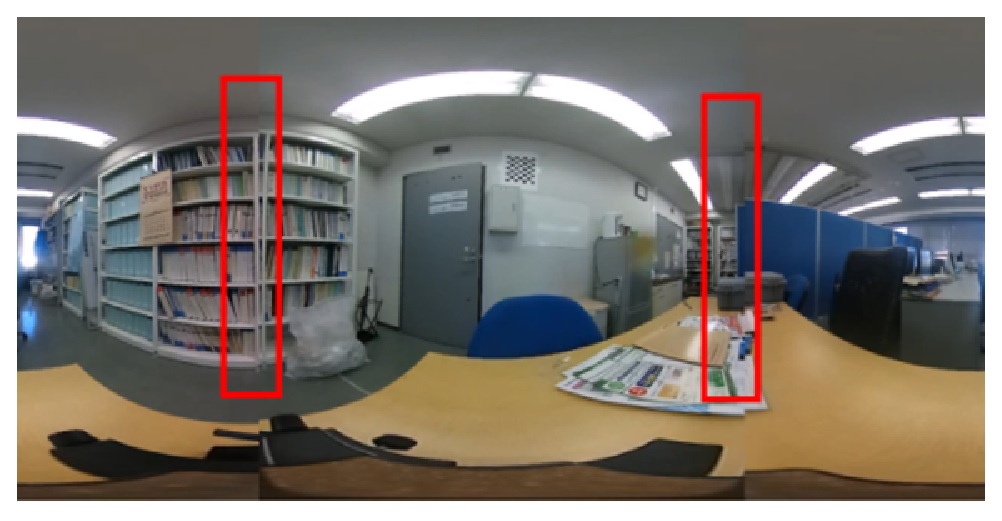
\includegraphics[width=12cm]{./Appendix/fig/Ocam.eps}
		\caption{OcamCamera Toolbox��p���Đ������������~���摜}
		\label{fig:Ocam}
	\end{center}
\end{figure}

���O�̌��؂ł́C��ʓI�ɍL���p�����Ă���L�p�J�����p�̓����p�����[�^�̍Z�����C�u�����ł���OCamCalib Toolbox\cite{scaramuzza2006}��p����THETA S��2�‚̋���J�����̓����p�����[�^�����ꂼ�ꐄ�肵�����~���摜�𐶐������ꍇ�ƁC�J�������������񋟂�������p�����[�^��p���Đ����~���摜�𐶐������ꍇ���r�����DOCamCalib Toolbox��p���Đ��肵�������p�����[�^�ɂ���Đ������������~���摜��}\ref{fig:Ocam}�Ɏ����D
�Ԃ��g�ň͂�ꂽ������2�‚̋���J�����摜�̂‚Ȃ��ڂɂ����邪�C�‚Ȃ��ڂɂ��ꂪ�������I��2�d�Ɍ����Ă��邱�Ƃ��m�F�ł���D����͐��肳�ꂽ�����p�����[�^�����f����\������̂ɕs�\���ł��邱�Ƃ������ł���D
����ɑ΂��C�J�������������񋟂�������p�����[�^��p���Đ������������~���摜��}\ref{fig:inpara}�Ɏ����D
���̏ꍇ�C2�‚̋���J�����̉f��������Ȃ��‚Ȃ����Ă��邱�Ƃ��킩��D���̂悤�ɐ����~���摜�����x�ǂ����܂��Ă��邱�Ƃ���C�J�����������̒񋟂�������p�����[�^�͋��̃��f�����\�����m�ɕ\���”\�ł���Ɣ��f���C�����p�����[�^�̂��ꓙ�ɂ��c�݂̕␳�͂��Ă��Ȃ��D


\begin{figure}[t]
	\begin{center}
		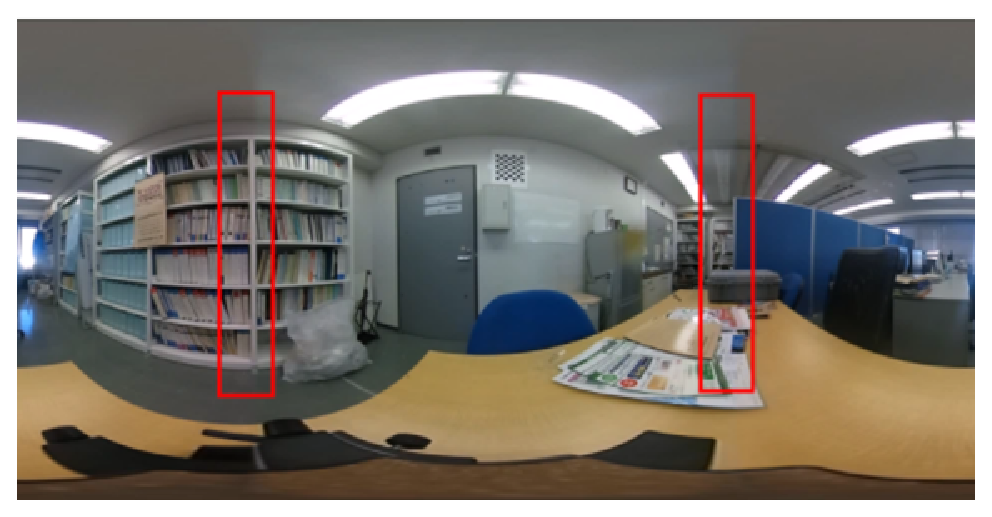
\includegraphics[width=12cm]{./Appendix/fig/inpara.eps}
		\caption{�J�����������̓����p�����[�^�ɂ���Đ������ꂽ�����~���摜}
		\label{fig:inpara}
	\end{center}
\end{figure}

\newpage

\addtocounter{chapter}{1}

%%%%%%%%%%%%%%%%%%%%%%%%%%%%%%%%%%%%%%%%%%%%%%%%%%%%%%%%%%%%%%%%%%%%%%%%%%%%%%%
%%% Local Variables:
%%% mode: katex
%%% TeX-master: "../thesis"
%%% End:

%%\chapter{水中Structure from Motionの研究との違いについて}
\lhead[付録B 水中Structure from Motionの研究との違いについて]{}
\setcounter{page}{1}
\renewcommand{\thepage}{B--\arabic{page}}

\thispagestyle{empty}

\newpage
%%%%%%%%%%%%%%%%%%%%%%%%%%%%%%%%%%%%%%%%%%%%%%%%%%%%%%%%%%%%%%%%%%%%%%%%%%%%%%%
\section{はじめに}




\newpage

\section{水中Structure from Motionの研究との違いについて}


\newpage


%%%%%%%%%%%%%%%%%%%%%%%%%%%%%%%%%%%%%%%%%%%%%%%%%%%%%%%%%%%%%%%%%%%%%%%%%%%%%%%
%%% Local Variables:
%%% mode: katex
%%% TeX-master: "../thesis"
%%% End:

%%\input{./Appendix/appendix_C}
\cleardoublepage
%
% 論文の最後
%
\end{document}